\Chapter{SOAR-based epidemiological model}\label{chapter:chapter2}

The simulated environment presented in this work was designed to resemble the environment described by Grey et al.\cite{grey2011procedural} which in turn used the implementation done by Prageeth Silva\cite{silva2010shadow}.
As of the time of writing, the original implementation of Shadow Quest used in evaluation of Grey's model is unavailable and so a custom implementation with modifications was made specifically for the sake of experimentation.
Each agent may occupy a single tile in a grid-based world.
The major difference between the work done by Grey et al. and the solution described in this thesis is the focus on information propagation.
For this reason the agents and their actions are adjusted to be compatible with the epidemiological models that can be used to model the propagation of information.
The temporal structure used in the design of the simulation is based on the concept of turns.
Because the interaction with a human player is not necessary to simulate the progression of a procedurally emergent plot, the turns are simply simulation steps.
Within a single turn all agents execute the aforementioned decision cycle, starting from receiving information regarding the state of the world around them, deciding on the action to perform and finally executing it.
The simulation used for evaluation of the model presented in this work is limited to a set of actions that each agent may perform.

\begin{itemize}
    \item Idle - agent does nothing, stays idle for the whole turn
    \item Move - agent may decide to move in one of the four cardinal directions by a single tile
    \item Infect - agent infects another agent
\end{itemize}

Because all agents execute their actions concurrently, conflicts may occur which the simulation engine must resolve.
For the sake of simplicity, a simple conflict resolution strategy was chosen where a random agent takes priority.
The second agent is overridden to have been idle for that turn.

In terms of an infection model the agent needs to be aware of the position of agents in its field of view as well as their state of infection.
Agents use inference to choose targets to follow and propose operators such as $Infect$ or $Walk$ dependent on the working memory.
The whole process starting with perception and ending with proposed operators is illustrated in figure \ref{fig:agent_think.drawio.png}.

\begin{figure}[H]
    \centering
    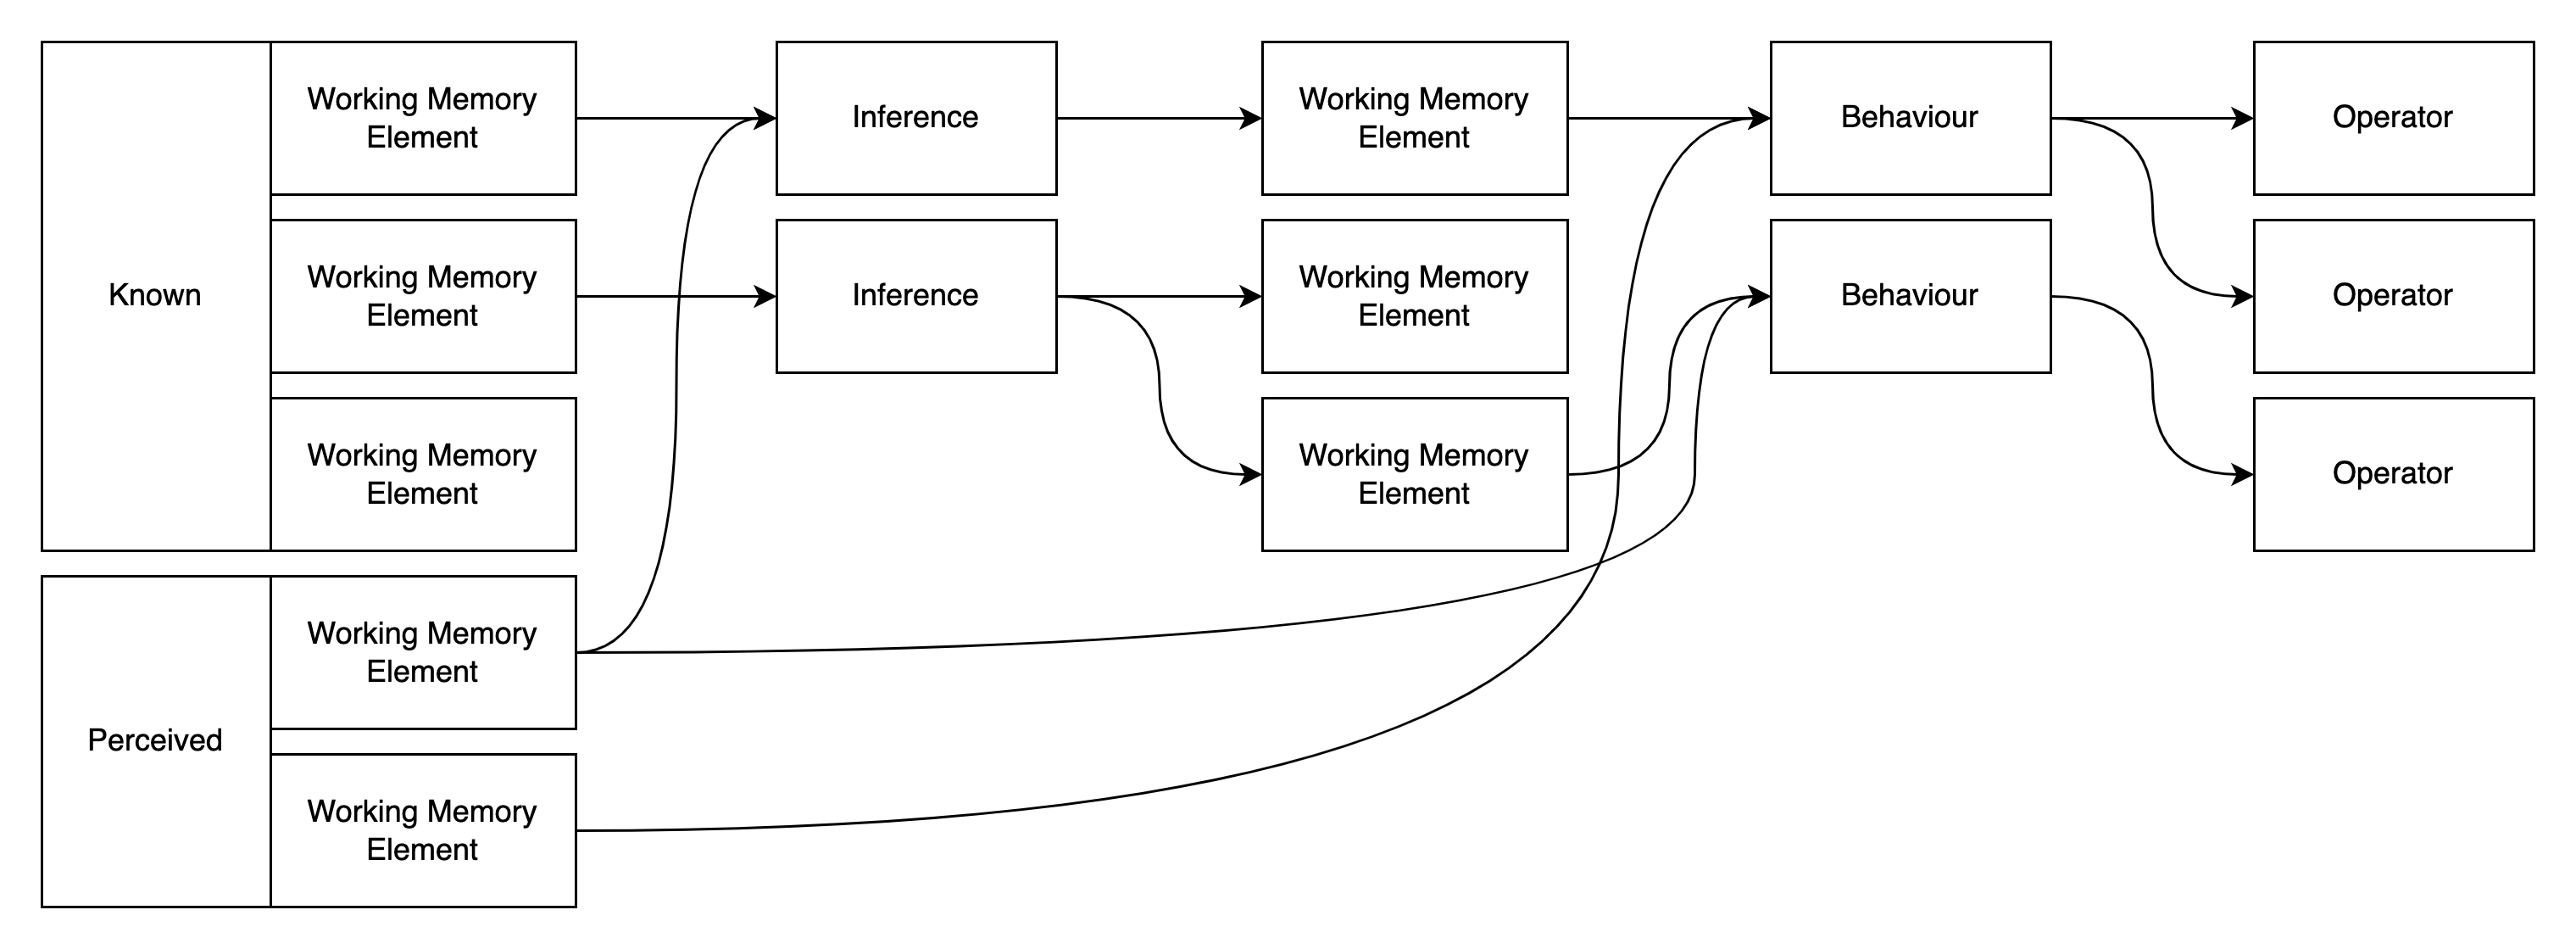
\includegraphics[width=1.0\textwidth]{images/chapter1/agent_think.drawio.png}
    \caption{Example agent's thinking process}\label{fig:agent_think.drawio.png}
\end{figure}

\section{Technical aspects of the implementation}

The SOAR cognitive architecture yields itself well to implementation using Entity-Component-System (ECS) approach.
The ECS pattern is a data-driven approach to game implementation where all logic is implemented as either components or systems \cite{raffaillac2019polyphony}.
An entity is a collection of components which in turn are containers of data that hold some state but no logic of their own.
The systems are functions that operate on entities based on some defined queries (such as all entities containing a component representing position and velocity) and then modify the state of the components.
This approach is performant as it allows for many otherwise impossible optimization techniques to be utilized (such as SIMD instructions and aggressive inlining)\cite{harkonen2019advantages}.
In the case of the cognitive architecture in question, the components would be working memory elements as well as inference and behavior rules.
A sensory system could be designed for feeding the working memory with the state of the world based on other components such as position, state, health or other types of data.
Another set of systems would run all inference rules and behavior rules and finally a system would evaluate operators proposed by the previous system and execute their actions.

The actual implementation of all simulations in this thesis is based on the MonoGame framework as described in the book "Introducing 2D Game Development in C\#"\cite{pavleas2013introducing}.
The ECS implementation used "a high-performance C\# based Archetype and Chunks Entity Component System (ECS) for game development and data-oriented programming" called Arch\cite{matthaeus2023arch}.
The reason for choosing this project over others is due to the results of performance analysis done by Paillat Laszlo in their ECS benchmark\cite{laszlo2023arch}.

Because the system is using an entity-component-system architecture, all experiment configurations are expressed through code by means of changing the values of components present on entities.
A $Sight$ component represents the sight of the agent and thus regulates how far it is able to see other agents.
The $SightSystem$ is then responsible for gathering all entities possessing the $WorkingMemory$, $Position$ and $Sight$ components and calculating the visibility of all the agents.
Two separate systems exist for processing inferences and behaviors called $InferenceSystem$ and $BehaviourSystem$ respectively.
The component responsible for proposing descriptors is called $Behaviour$ while inferences are stored within the $Inference$ component.
For the sake of implementation of the epidemiological model all agents possess the $Infection$ component that stores their current state as well as the lifetime after infection.

\section{Implementation of infection model}

Social media and information propagation are similar in nature to epidemiological phenomena.
It is common to refer to a fast spreading news as being viral, referring to its ability to spread from host to host rapidly.
In epidemiology the simplest approach to model how a disease spreads is to use a compartmental model that divides the population into compartments or categories and then assigns each compartment a mathematical description of its population size over time.
Modeling the spread of infectious diseases has long been the goal of many scientists\cite{liu2016}.
The simplest and most popular model is based on the partitioning of a population in three compartments of susceptible, infected and recovered\cite{weiss2013sir}.
This model is called SIR and consists of three differential equations describing each compartment.
Figure \ref{fig:sir.drawio.png} illustrates possible state transitions within the SIR model.

\begin{figure}[H]
    \centering
    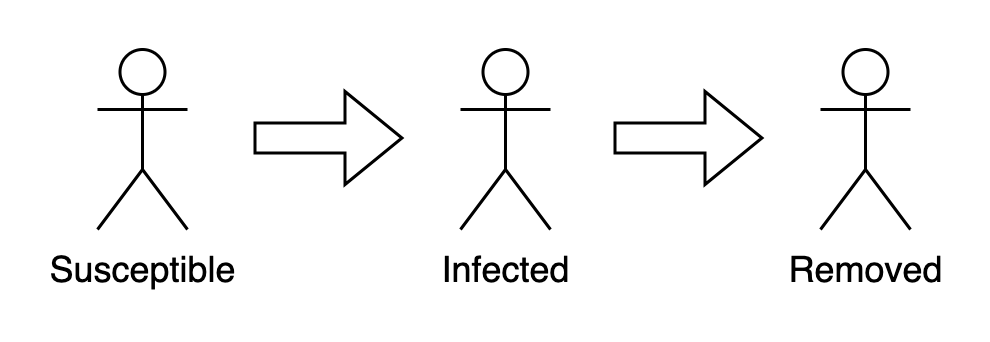
\includegraphics[width=0.6\textwidth]{images/chapter2/sir.drawio.png}
    \caption{Agent state transition in SIR model}\label{fig:sir.drawio.png}
\end{figure}

\begin{equation} \label{eq:sir1}
    \frac{{dS}}{{dt}} = -\frac{{\beta \cdot S \cdot I}}{{N}}
\end{equation}

\begin{equation} \label{eq:sir2}
    \frac{{dI}}{{dt}} = \frac{{\beta \cdot S \cdot I}}{{N}} - \gamma \cdot I
\end{equation}

\begin{equation} \label{eq:sir3}
    \frac{{dR}}{{dt}} = \gamma \cdot I
\end{equation}

Equations \ref{eq:sir1}, \ref{eq:sir2} and \ref{eq:sir3} describe how each compartment of the population changes over time.
The parameters of the model are:

\begin{itemize}
    \item $S$: Number of susceptible individuals in the population
    \item $I$: Number of infected individuals
    \item $R$: Number of recovered individuals
    \item $N$: Total population size ($N = S + I + R$)
    \item $\beta$: Infection rate, determining the probability of a susceptible individual becoming infected when coming into contact with an infected individual
    \item $\gamma$: Recovery rate, indicating the average rate at which infected individuals recover and become immune
\end{itemize}

Variations of this model exist that aim to improve its representativeness in the real world usually by adding another partition group such as hibernator in SIHR\cite{zhao2012sihr}.
While the origins of these models stems from simulation of infectious diseases spreading across a population, many authors realized that social media and rumors can be modeled exactly the same way.
The SIHR model for instance is an example of a "rumor spreading model in social networks"\cite{zhao2012sihr}.
Another variant of the simple SIR model is SCIR, in which the letter 'C' stands for contacted and 'R' stands for refractory.
This model is used to analyze the impact of the "retweeting mechanism for online social media"\cite{xiong2012scir}.
Some authors use the concept of cellular automata to implement simulations of the spread of rumors or diseases\cite{silva2020}.
Because the name of the last group "recovered" is more strongly associated with diseases and epidemiological modeling, in this thesis a more general naming was adapted and the last group is called "removed" to indicate that the members of the population within that compartment do not take part in the simulation anymore.

Because the scope of this thesis is limited to application of such models in games, the aim of the proposed model is not to be as accurate in representation of real world disease spread but to be able to represent the idea behind modeling the spread of rumors or diseases in video games.
The most important aspect of the evaluation is the ability to express the standard SIR model using the cognitive architecture proposed in the preceding chapter.
For this reason a population is a multi-agent system where each agent can be susceptible or infected.
The agents have two defined behavior rules.
The first one can be summarized as "if not in contact with previously uncontacted agent and possessing message, go towards closest uncontacted agent".
Whereas second one is "if in contact with previously uncontacted agent and possessing message, make contact".
The action of contact is modeled using the $Tell$ operator with an arbitrary message.
The message plays no special role in the simulation and instead represents either a rumor or a disease being spread.
The condition that checks for the possession of the message is the one that differentiates infected agents from susceptible ones.
It is worth to note that in order for the simulation to produce any results, at least one agent must be initialized with the possession of the message (infection).
In general the logic expressed by the combination of previously defined behavior and inference rules can be illustrated using a flowchart shown in figure \ref{fig:sir_logic.drawio.png}.

The configuration of the system for each experiment is possible by either changing the numerical values of system's parameters or modifying the list of behavior and inference rules that each agent possesses.
The numerical parameters include the sight distance of the agents, their lifetime once infected and the size of the population which influences the density of agent's random distribution.
For experiments 1-4 the sight of the agents is set at 8 tiles of distance and the population size is 40 agents.

% TODO: Range limited movement

\subsection{Choosing parameters for the epidemiological model}

Optimization of system's parameters to match the dynamics of the epidemiological model's arbitrary combination of parameters is out of the scope of this thesis.
The epidemiological model exists only to compare the dynamics of the population's behavior against and not to produce results that closely match the exact results obtained from the mathematical model.
For this reason the choice of parameters for the epidemiological model was arbitrary and a matching combination of system's parameters was chosen by trail and error.

In the case when a specific dynamics of a given combination of SIR model parameters is desired, the implementing person should manually optimize the system's parameters until the resultant simulation dynamics match the mathematical model.
It is possible to find out the SIR model's parameters based on the results of a population's simulations however by solving the system of equations.
In order to estimate the values for the parameters of the SIR model, a simple optimization technique for minimization of sum of squares of errors could be used.
Nelder-Mead is a popular optimization algorithm used for unconstrained optimization problems such as this one\cite{singer2009nelder}.
The implementation of this technique is outside the scope of this thesis.

\subsection{Visibility and memorization of agents' positions}

All agents that posses the $Sight$ component can perceive other agents in the simulation granted they are within the defined range.
An agent remembers the positions of all agents that it has seen at least once.
During each behavior and inference processing step, the working memory contains both the list of remembered agents' positions as well as the list of currently visible agents and the remembered state of infection for each of them.
If the agent sees another agent that it saw before, its old position and remembered infection state is overridden by the new position and infection state.
Figure \ref{fig:images/visibility/agent47.png} shows a visualization of $Agent47$'s ability to perceive other agents in its range of sight.

\begin{figure}[H]
    \centering
    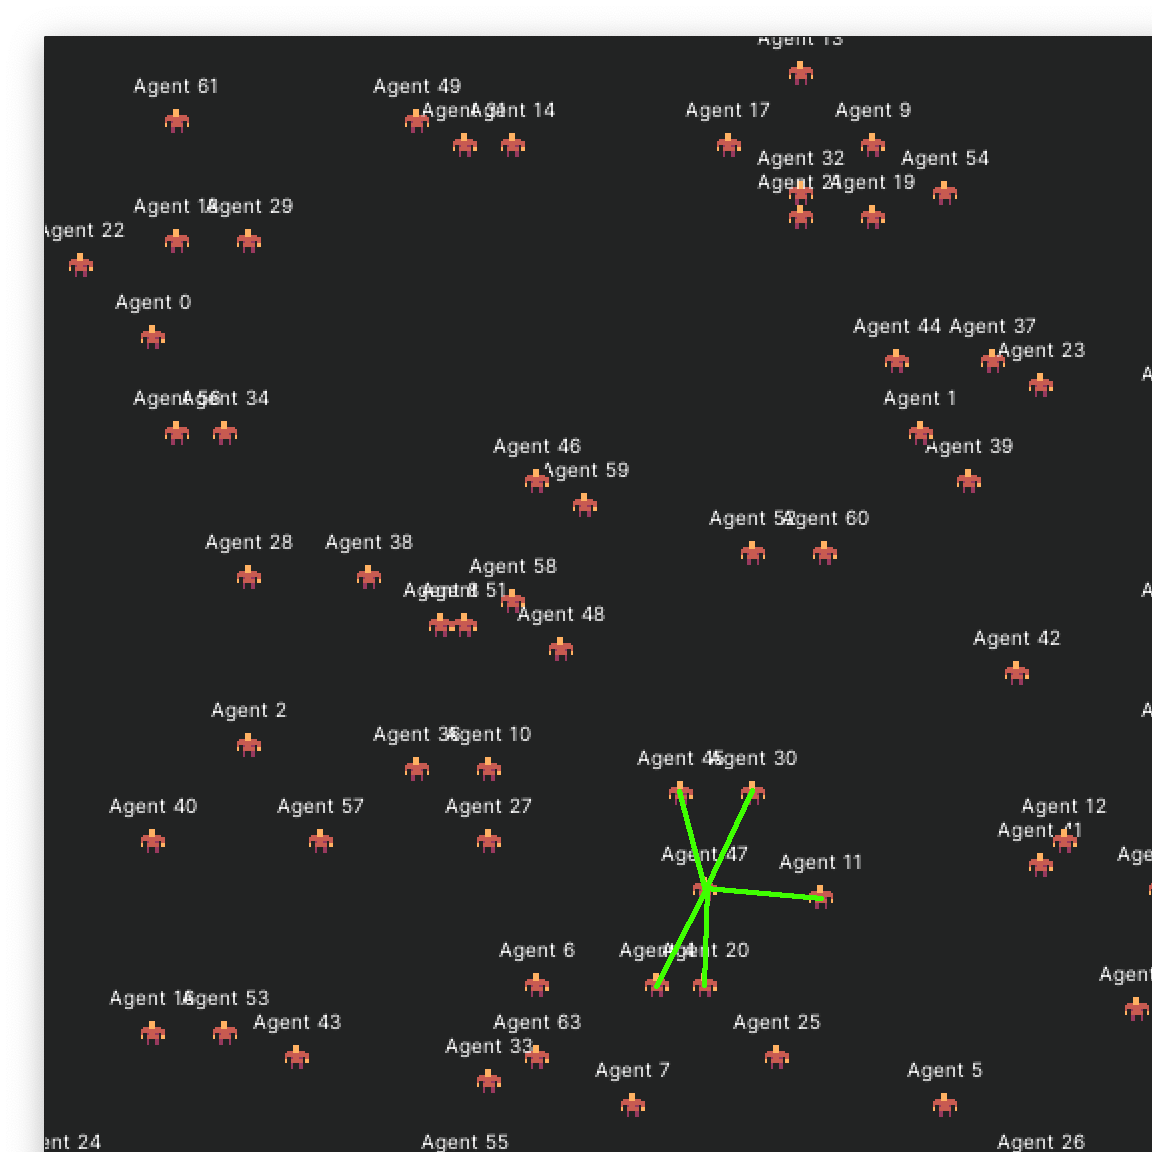
\includegraphics[width=0.5\textwidth]{images/visibility/agent47.png}
    \caption{Visualization of the agent's ability to perceive other agents in range of sight}\label{fig:images/visibility/agent47.png}
\end{figure}

After $Agent11$ leaves the range of $Agent47$'s sight, it is no longer perceived by them and instead a last remembered position remains in the $Agent47$'s working memory.
Figure \ref{fig:images/visibility/agent47_moved.png} illustrates the state of $Agent47$'s perception after $Agent11$ left the periphery of their vision.

\begin{figure}[H]
    \centering
    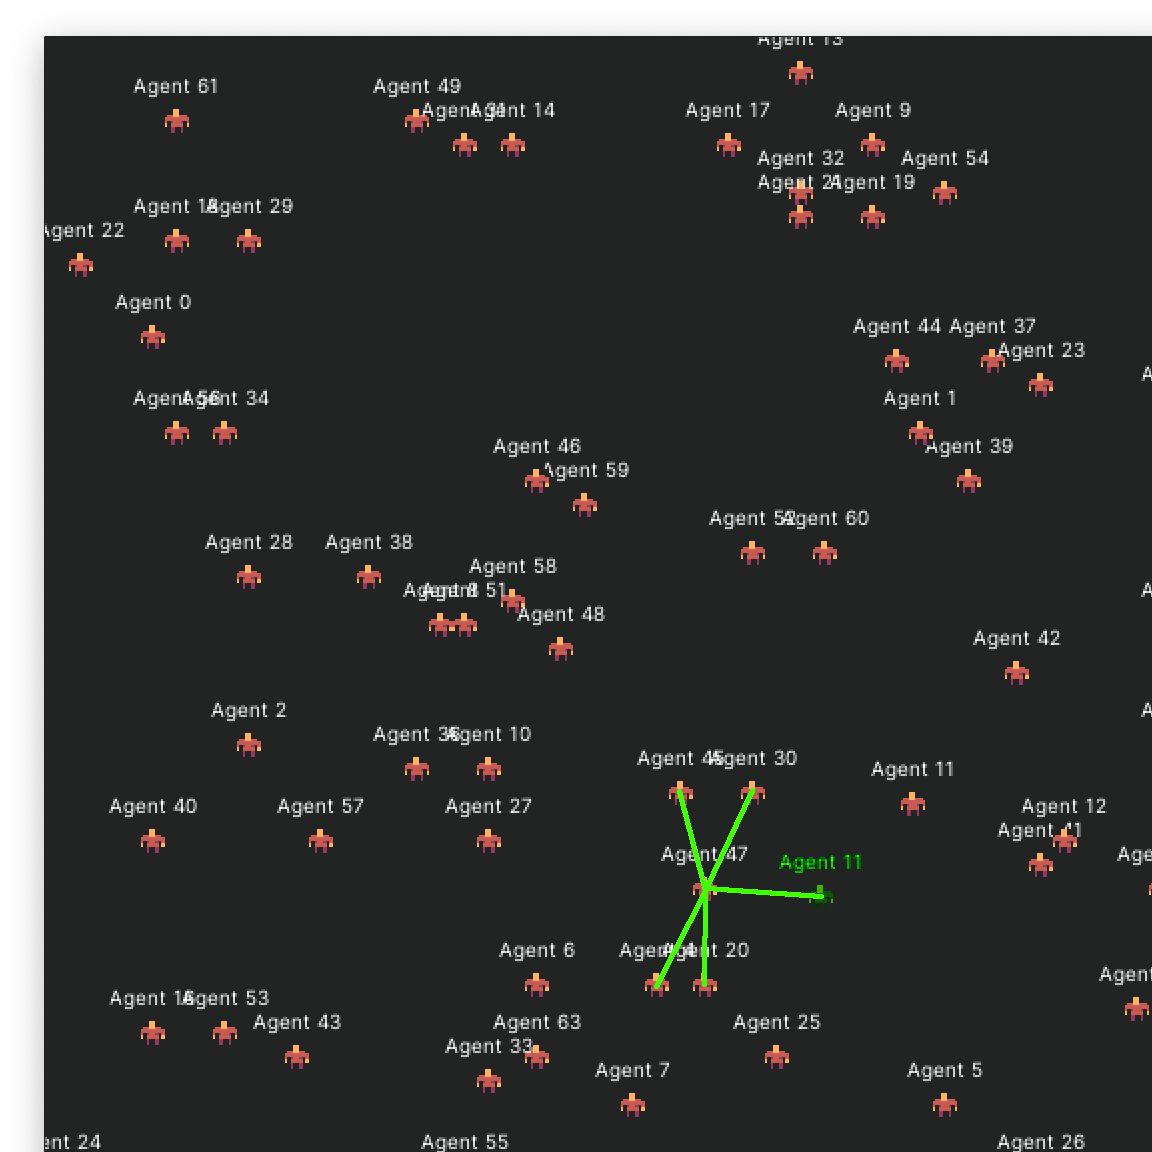
\includegraphics[width=0.5\textwidth]{images/visibility/agent47_moved.png}
    \caption{Visualization of the agent's ability to remember agent's last position}\label{fig:images/visibility/agent47_moved.png}
\end{figure}

\subsection{Experiment 1 - semi-static agents}

\begin{figure}[H]
    \centering
    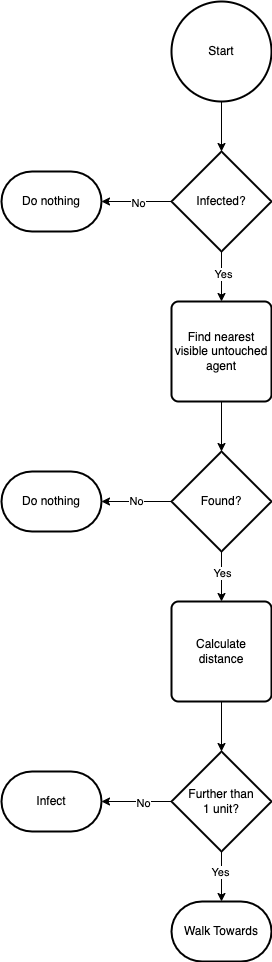
\includegraphics[width=0.3\textwidth]{images/chapter2/sir_logic.drawio.png}
    \caption{Flowchart representing logic expressed by agent behavior rules, terminal blocks represent operators being proposed by the agent}\label{fig:sir_logic.drawio.png}
\end{figure}

The simulation starts with a single agent being infected and the rest of the agents randomly distributed in a rectangular area.
The initial state is visible on figure \ref{fig:images/chapter2/sir0/sir_1.png}.
The first experiment assumes each agent can see other agents that are up to 8 tiles away from it and that no agent can ever become removed.
Immediately in the second step of the simulation, the infected agent met up with an adjacent agent and infected them.
Soon after two clusters of agents formed, each with agents trying to touch each other first before moving on.
The two clusters are visible on figure \ref{fig:images/chapter2/sir0/sir_28.png}.
After 71 simulation steps nearly all agents have been infected and strong clustering behavior is clearly visible (figure \ref{fig:images/chapter2/sir0/sir_71.png}).
Figure \ref{fig:images/chapter2/sir0/sir_85.png} shows the final state of the simulation after 85 steps where all agents have become infected and there are no remaining survivors.

\begin{figure}[H]
    \centering
    \subfigure[Step 1]{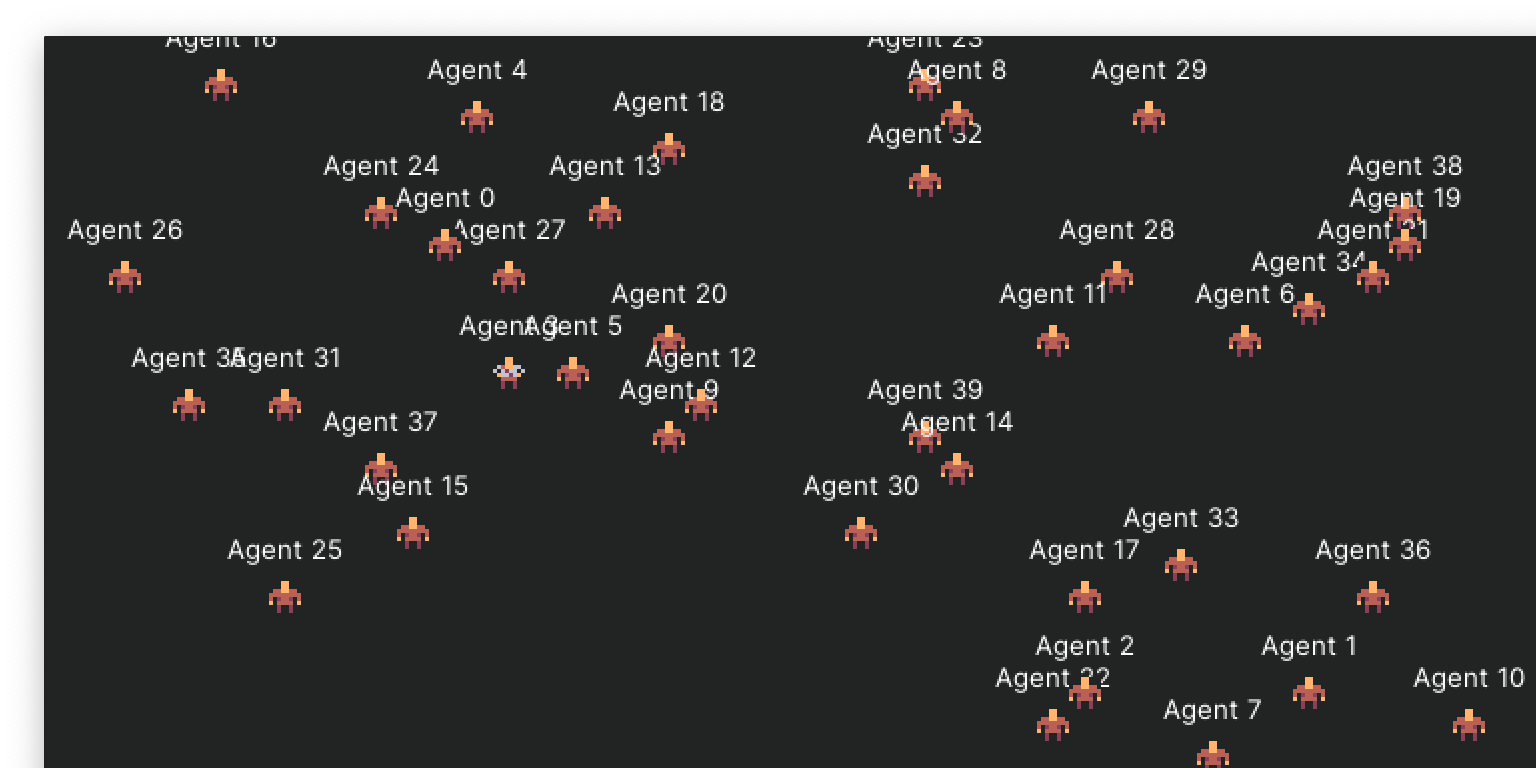
\includegraphics[width=0.48\textwidth]{images/chapter2/sir0/sir_1.png}\label{fig:images/chapter2/sir0/sir_1.png}}
    \hspace*{\fill}
    \subfigure[Step 28]{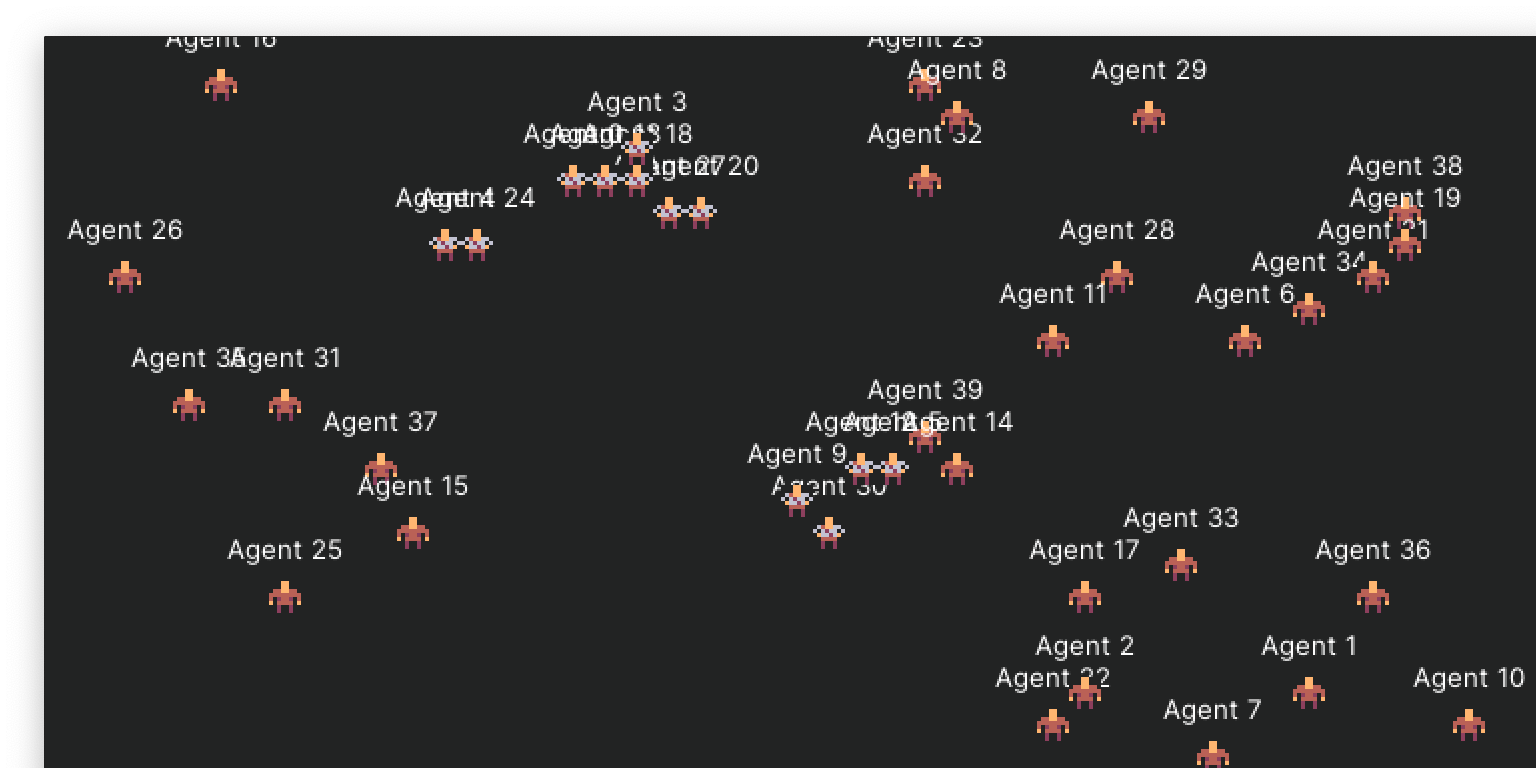
\includegraphics[width=0.48\textwidth]{images/chapter2/sir0/sir_28.png}\label{fig:images/chapter2/sir0/sir_28.png}}

    \subfigure[Step 71]{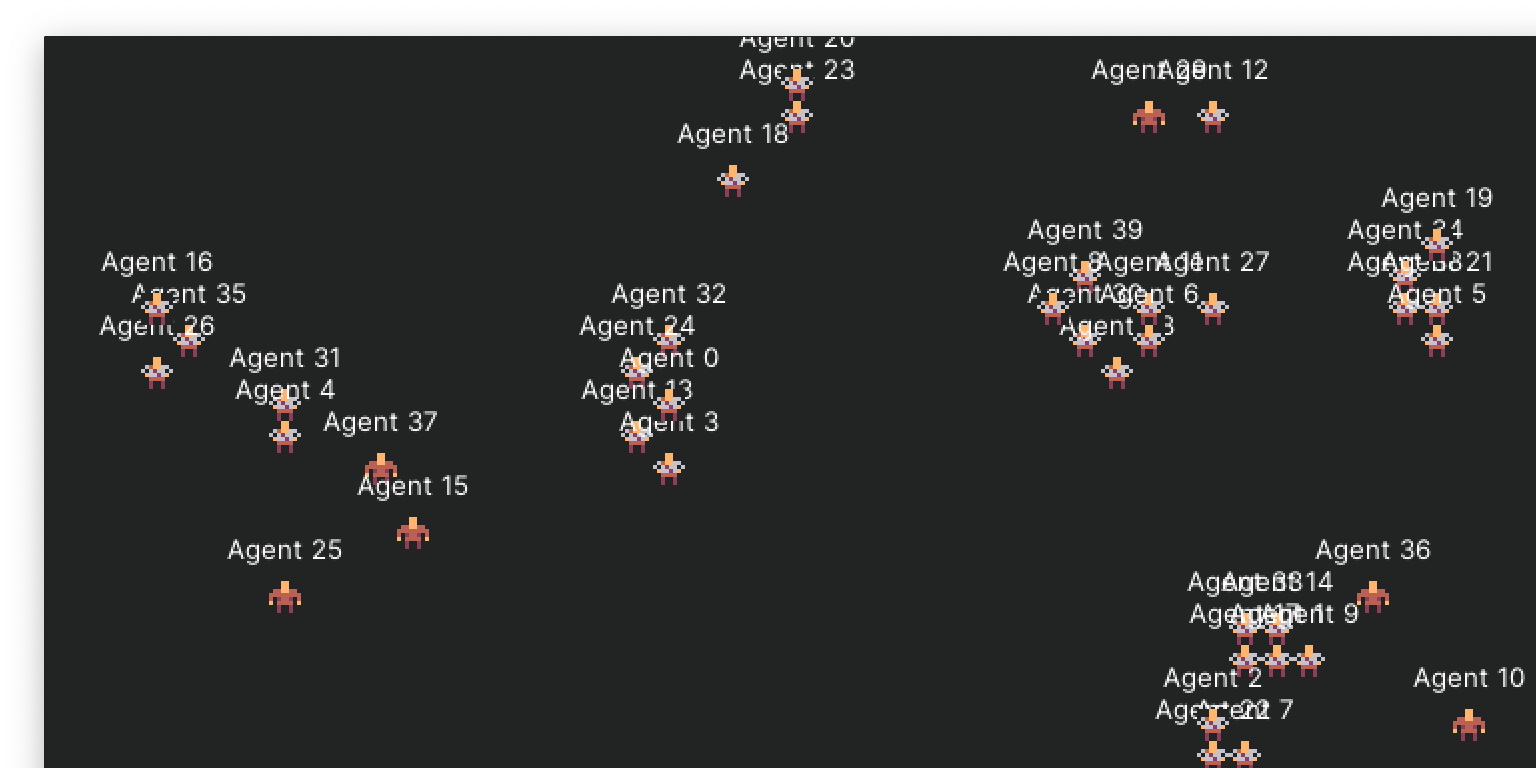
\includegraphics[width=0.48\textwidth]{images/chapter2/sir0/sir_71.png}\label{fig:images/chapter2/sir0/sir_71.png}}
    \hspace*{\fill}
    \subfigure[Step 85]{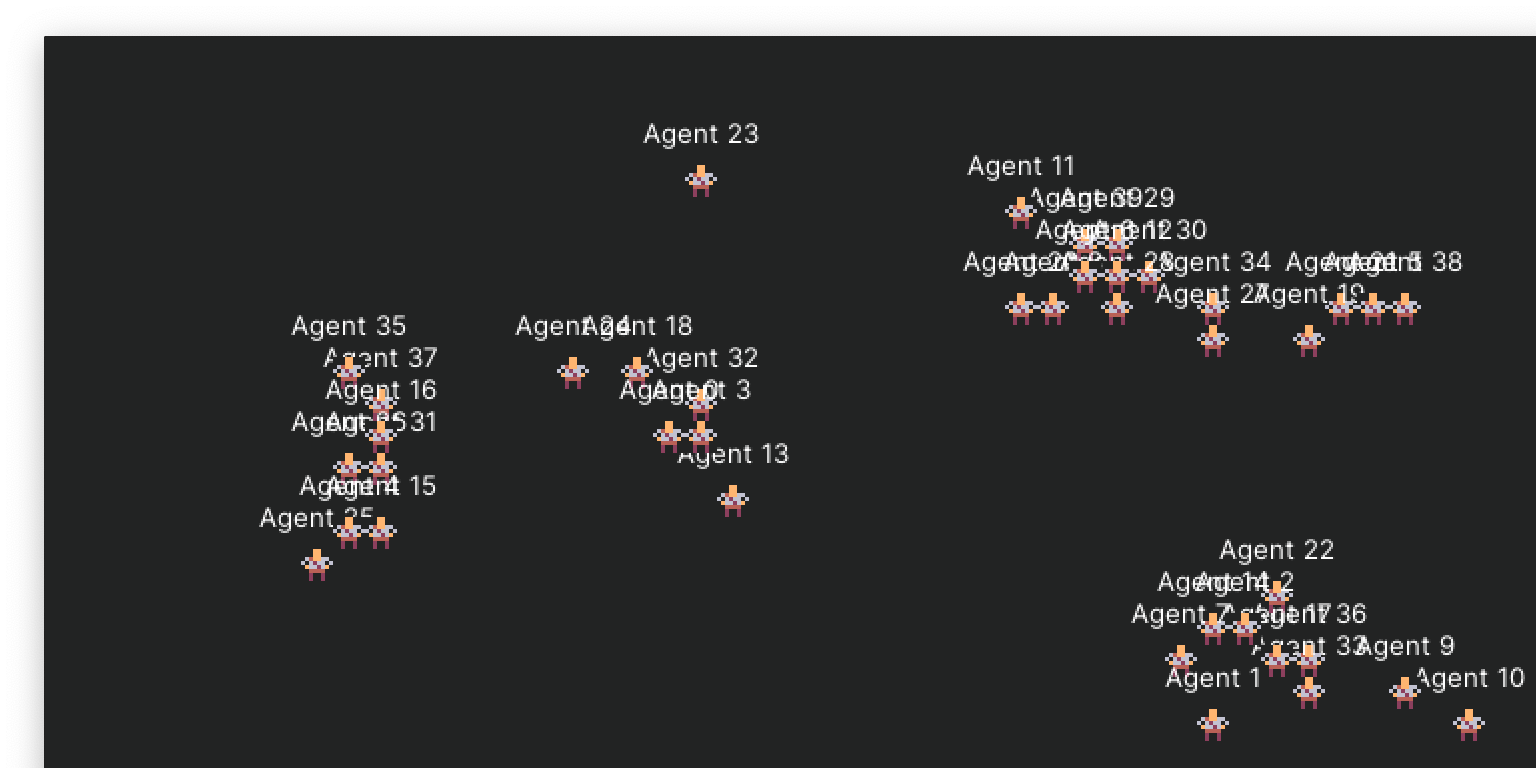
\includegraphics[width=0.48\textwidth]{images/chapter2/sir0/sir_85.png}\label{fig:images/chapter2/sir0/sir_85.png}}

    \caption{Experiment 1} \label{fig:experiment0}
\end{figure}

Due to the behavior rule specifying that each agent should try to meet with each previously unmet agent that was seen at least once, the agents will form clusters and thus potentially separate themselves further away from other healthy individuals.
While it might seem like a strange behavior in an epidemic model, it might make sense to consider it in terms of information propagation as humans have natural tendencies to form groups of interest.
So far the simulation assumed that agents that were not infected would remain still and do nothing.
This combined with the limited sight of the agents means that the simulation may stabilize in such a way that a survivor or group of survivors would remain undisturbed because of random distribution of agents.
An example of this situation is visible in figure \ref{fig:images/chapter2/sir0/sir_255.png}.
A slight modification of the behavior rules will make them instead choose a random direction to go which should decrease possibility of the model stabilizing in a state where survivors remain in the simulation because no infected agent came close enough to them.

\begin{figure}[H]
    \centering
    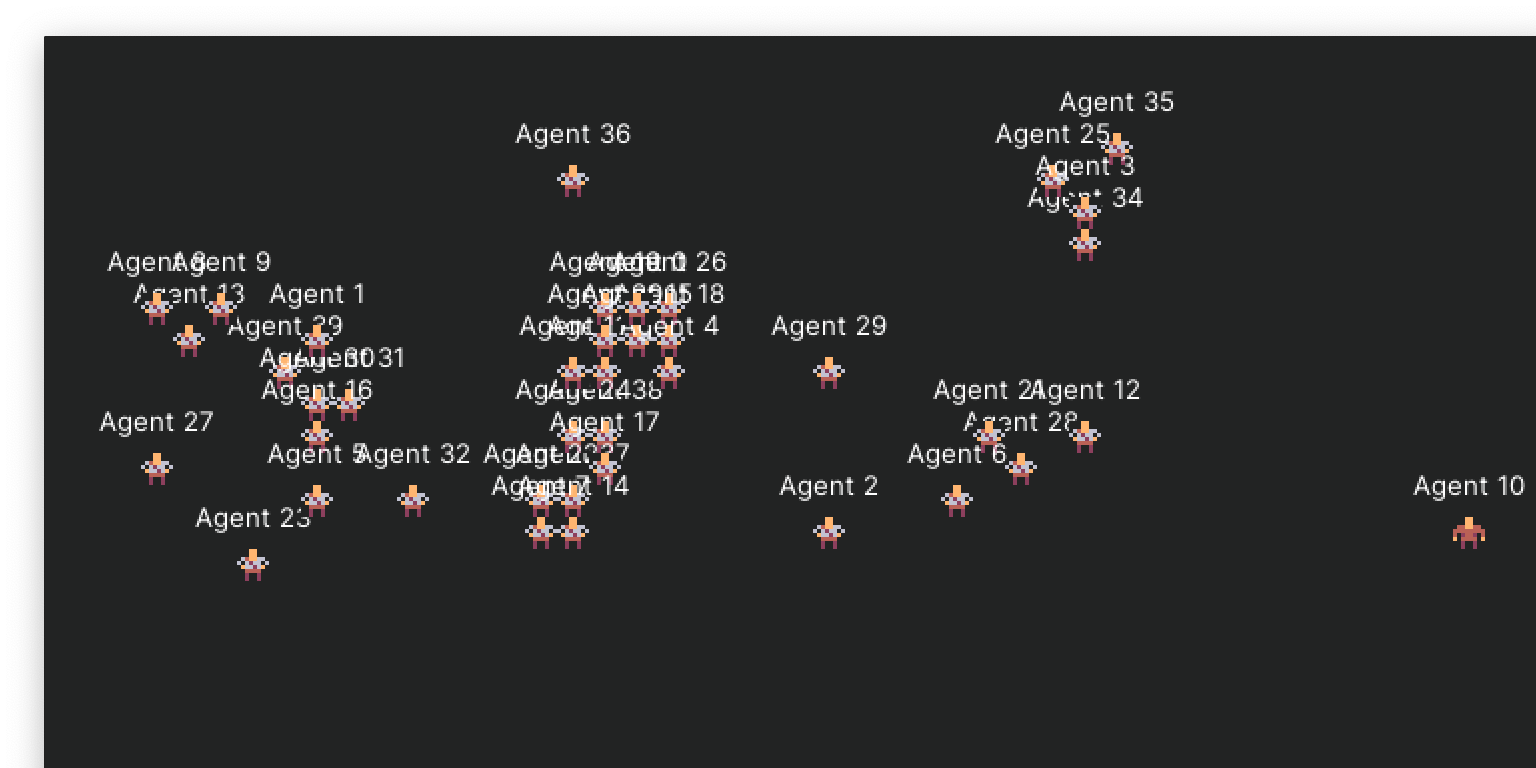
\includegraphics[width=1.0\textwidth]{images/chapter2/sir0/sir_255.png}
    \caption{Experiment 1 - lone survivor}\label{fig:images/chapter2/sir0/sir_255.png}
\end{figure}

\subsection{Experiment 2 - roaming agents without recovery}

After modification of the behavior rules to make susceptible individuals move around randomly as well as addition of a new rule that prevents the infected agent from targeting other infected agents the clustering behavior is gone.
Figure \ref{fig:images/chapter2/sir1/sir_123.png} shows the final state of the experiment with the new ruleset.
The distribution of the agents is more homogeneous than before, even though slight clustering still occurs.
The population size plotted against time on figure \ref{fig:images/chapter2/sir1/sir.png} matches with the SIR model plotted on figure \ref{fig:images/chapter2/experiment2.png} with parameters $\beta = 0.1, \gamma = 0.0, N = 40$.
The new rules produce behavior as illustrated by flowchart shown on figure \ref{fig:sir_logic2.drawio.png}.

\begin{figure}[H]
    \centering
    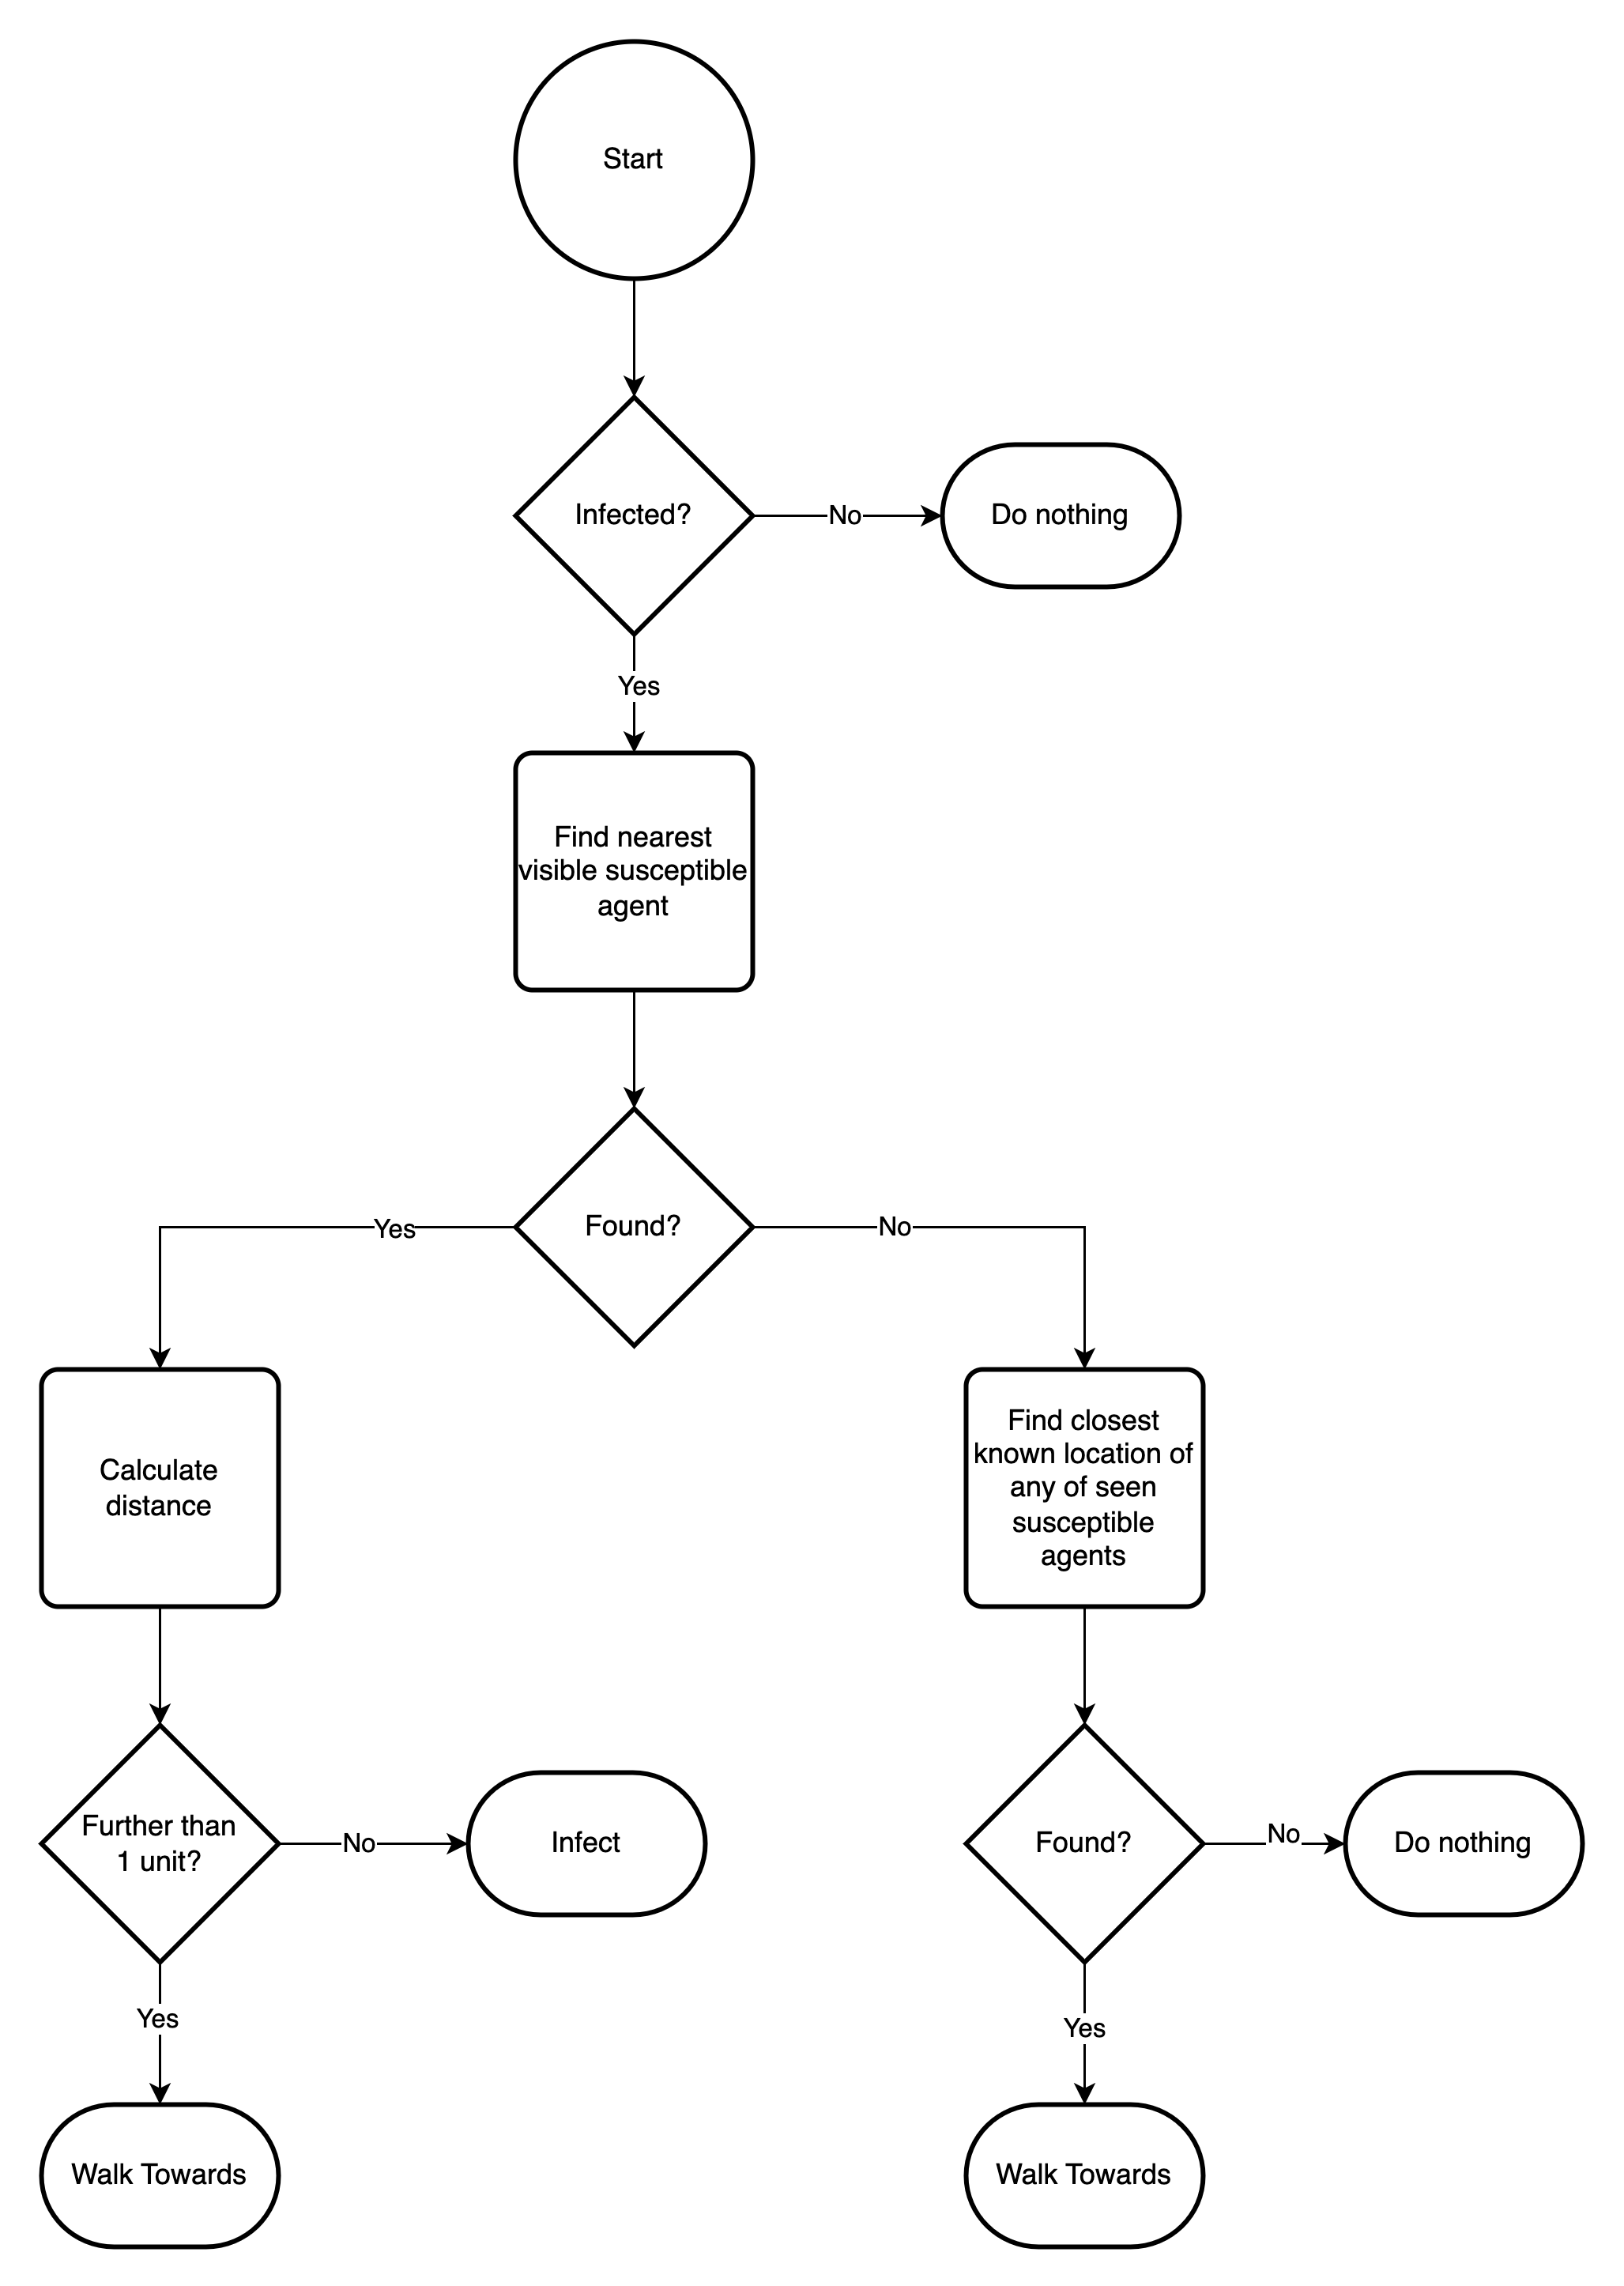
\includegraphics[width=0.6\textwidth]{images/chapter2/sir_logic2.drawio.png}
    \caption{Flowchart representing logic expressed by agent behavior rules, terminal blocks represent operators being proposed by the agent}\label{fig:sir_logic2.drawio.png}
\end{figure}

% Experiment 2

% \begin{figure}[H]
%     \centering
%     \subfigure[Experiment]{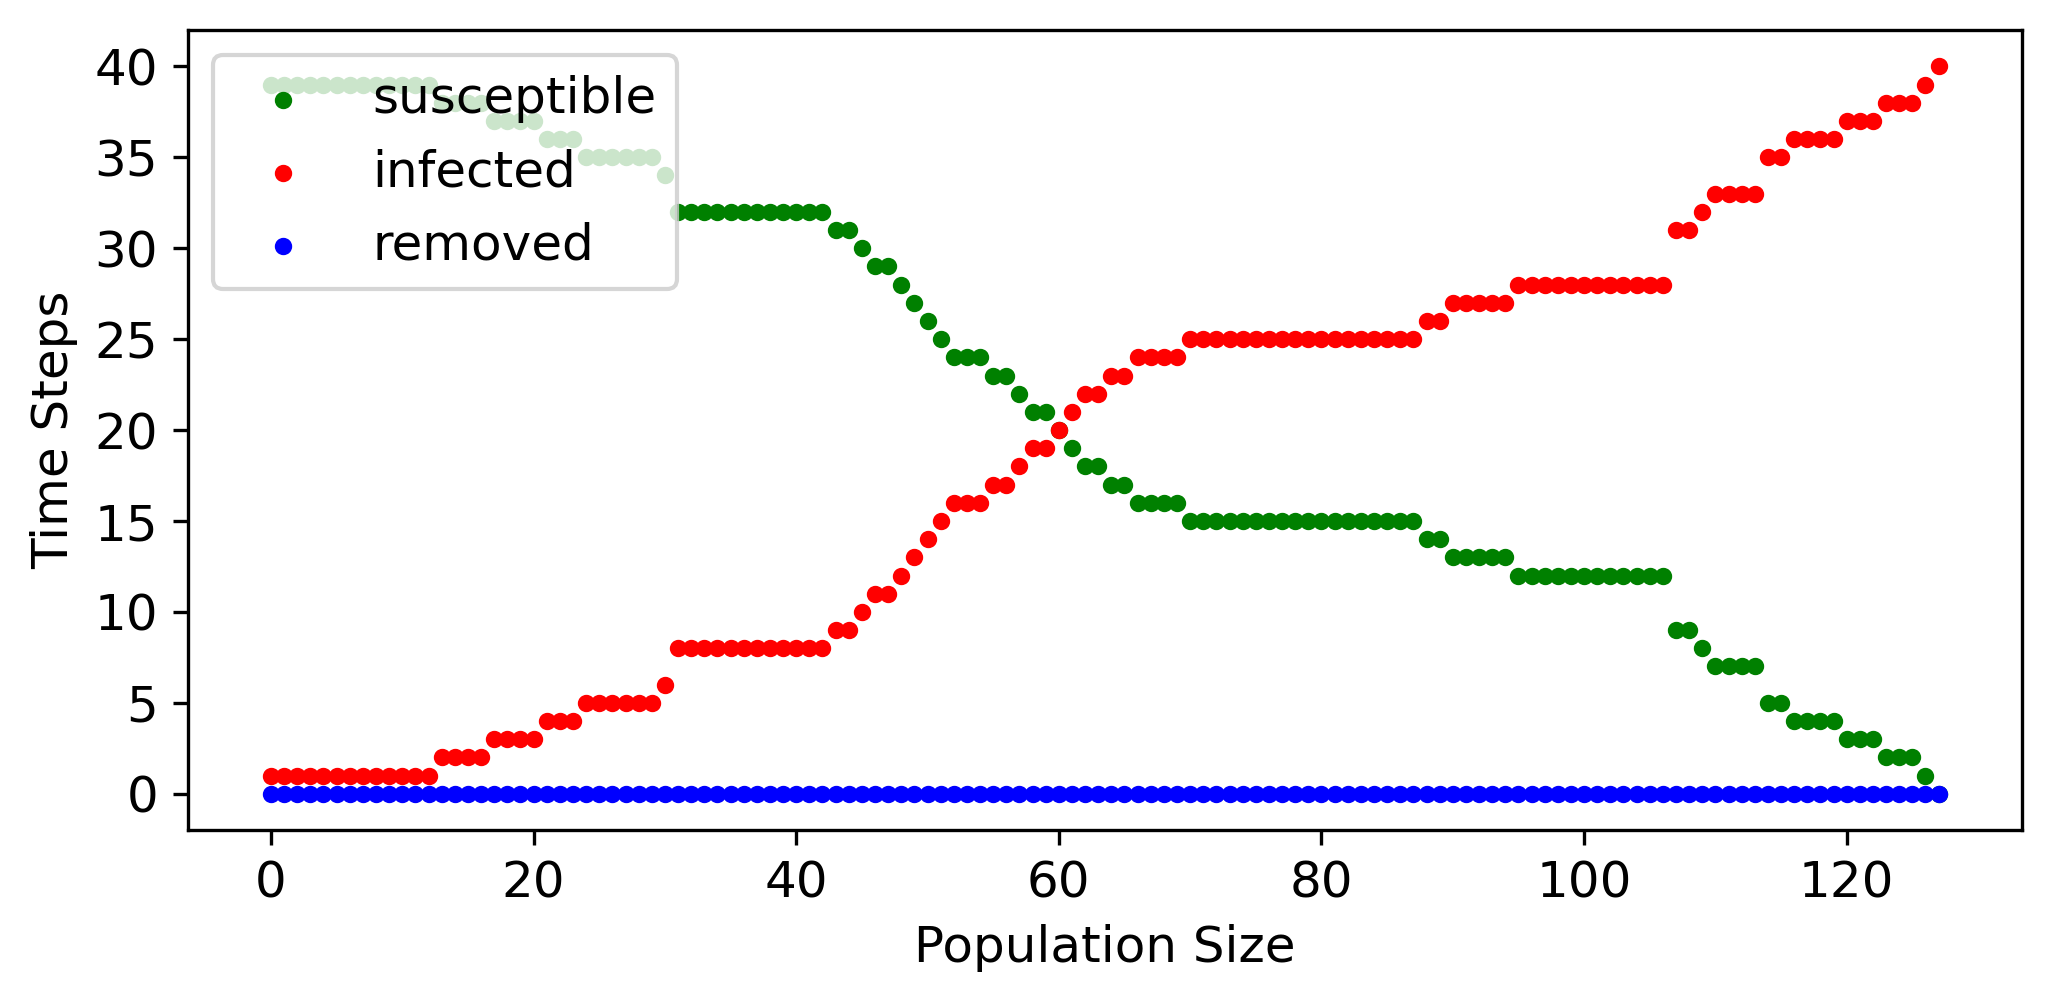
\includegraphics[width=0.48\textwidth]{images/chapter2/sir1/sir.png}\label{fig:images/chapter2/sir1/sir.png}}
%     \hspace*{\fill}
%     \subfigure[$\beta = 0.07, \gamma = 0.0, N = 40$]{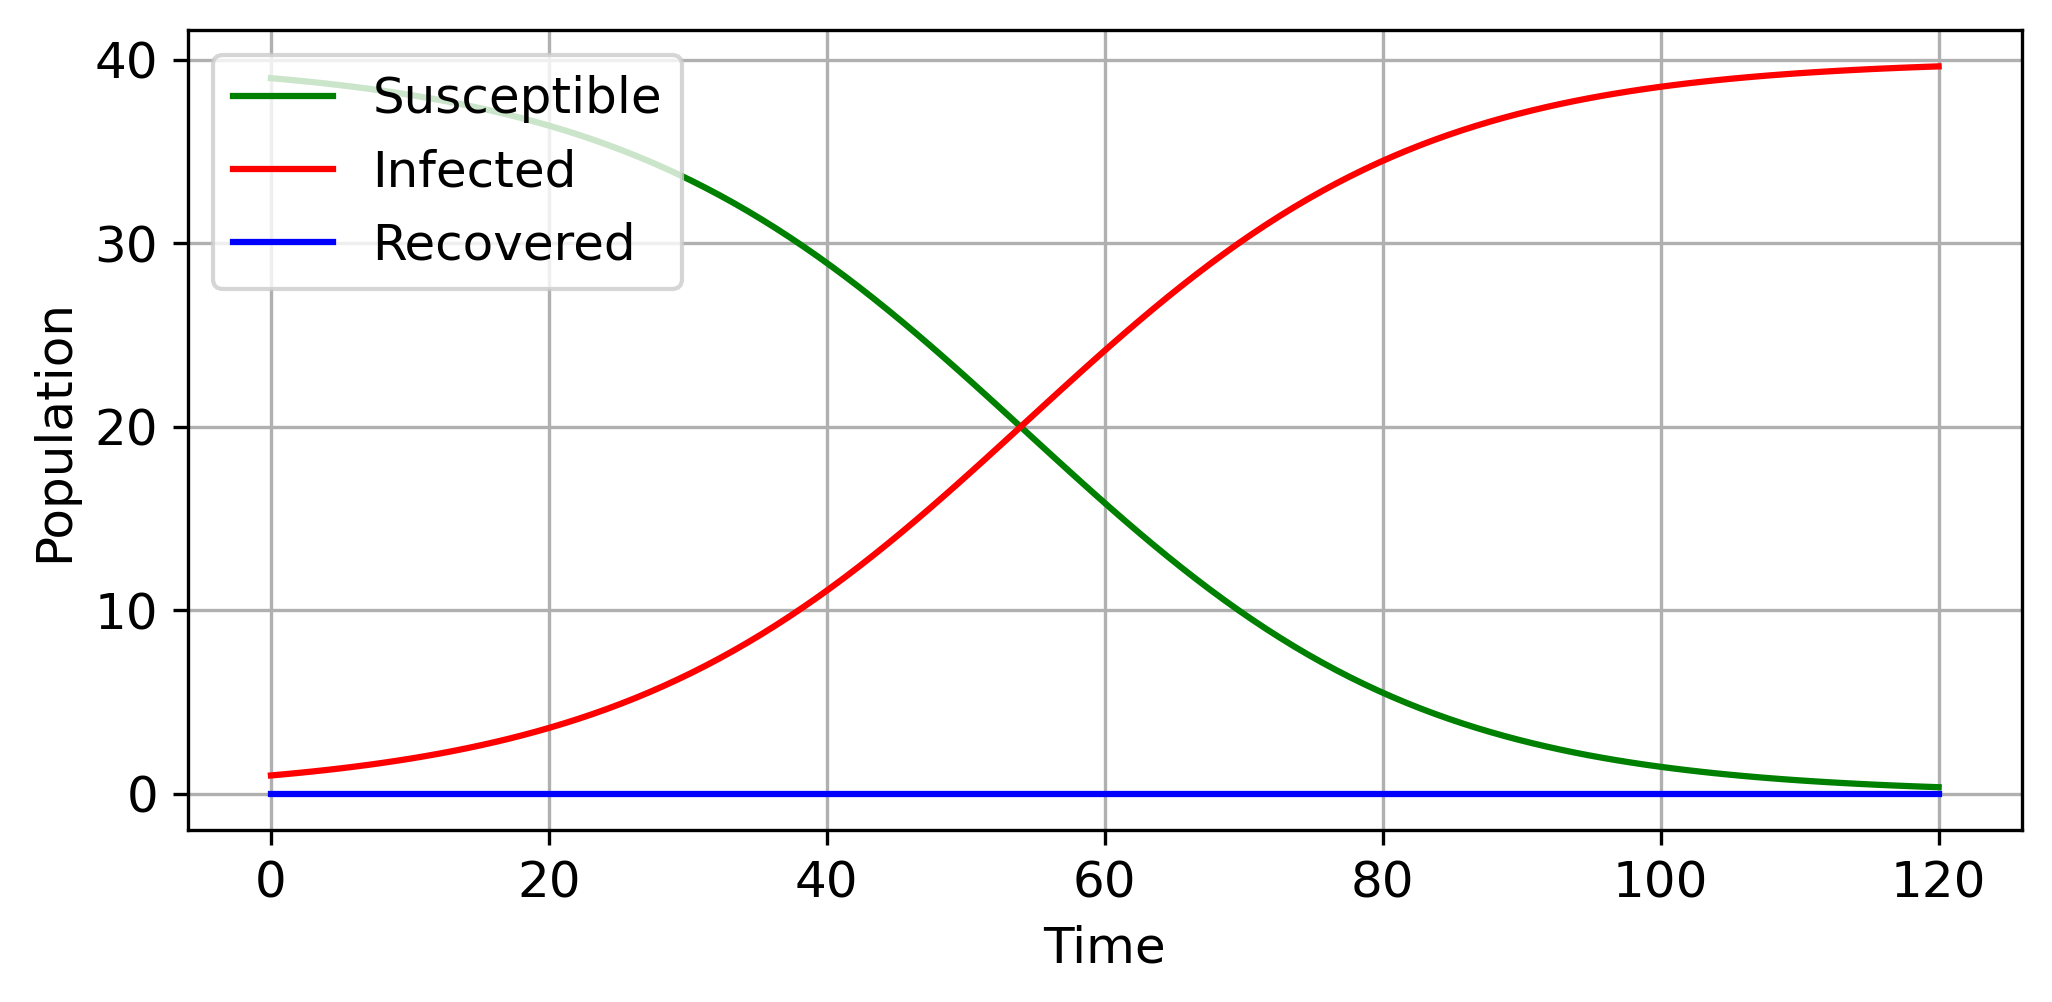
\includegraphics[width=0.48\textwidth]{images/chapter2/sir_ref/sir_1.png}\label{fig:images/chapter2/sir_ref/sir_1.png}}
%     \caption{Experiment 2 - SIR vs Experiment} \label{fig:experiment1-diagrams}
% \end{figure}

\begin{figure}[H]
    \centering
    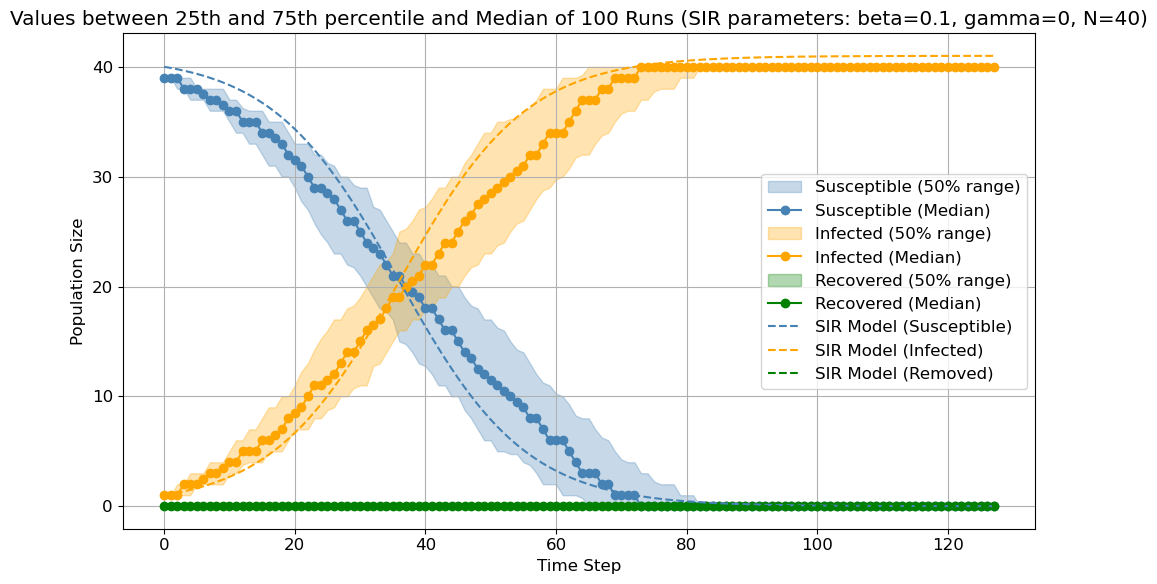
\includegraphics[width=1.0\textwidth]{images/chapter2/experiment2.png}
    \caption{Experiment 2 - population size over time}\label{fig:images/chapter2/experiment2.png}
\end{figure}

The initial state of the experiment shown on figure \ref{fig:images/chapter2/experiment2.png} is the same as with every other experiment.
The agents are randomly distributed and form three visually identifiable segments.
After the simulation starts infected agents quickly form a cluster in the bottom right corner as visible on figure \ref{fig:images/chapter2/sir1/sir_33.png}.
Soon after the cluster disperses and the agents move on to infect the rest of the population.
Finally, after 128 simulation steps, the whole population is infected and there are no more remaining survivors (figure \ref{fig:images/chapter2/sir1/sir_123.png}).

\begin{figure}[H]
    \centering
    \subfigure[Step 1]{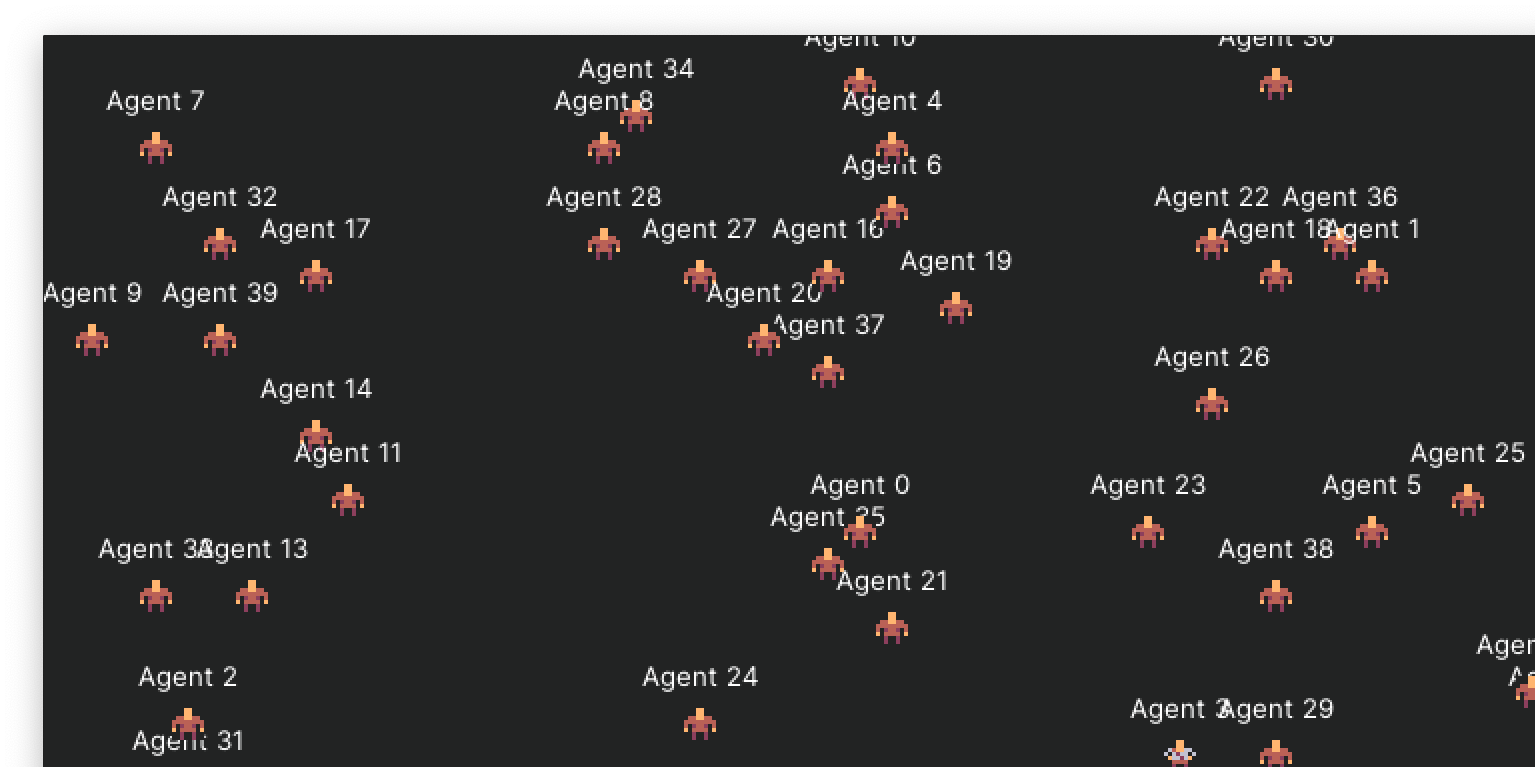
\includegraphics[width=0.3\textwidth]{images/chapter2/sir1/sir_1.png}\label{fig:images/chapter2/sir1/sir_1.png}}
    \hspace*{\fill}
    \subfigure[Step 33]{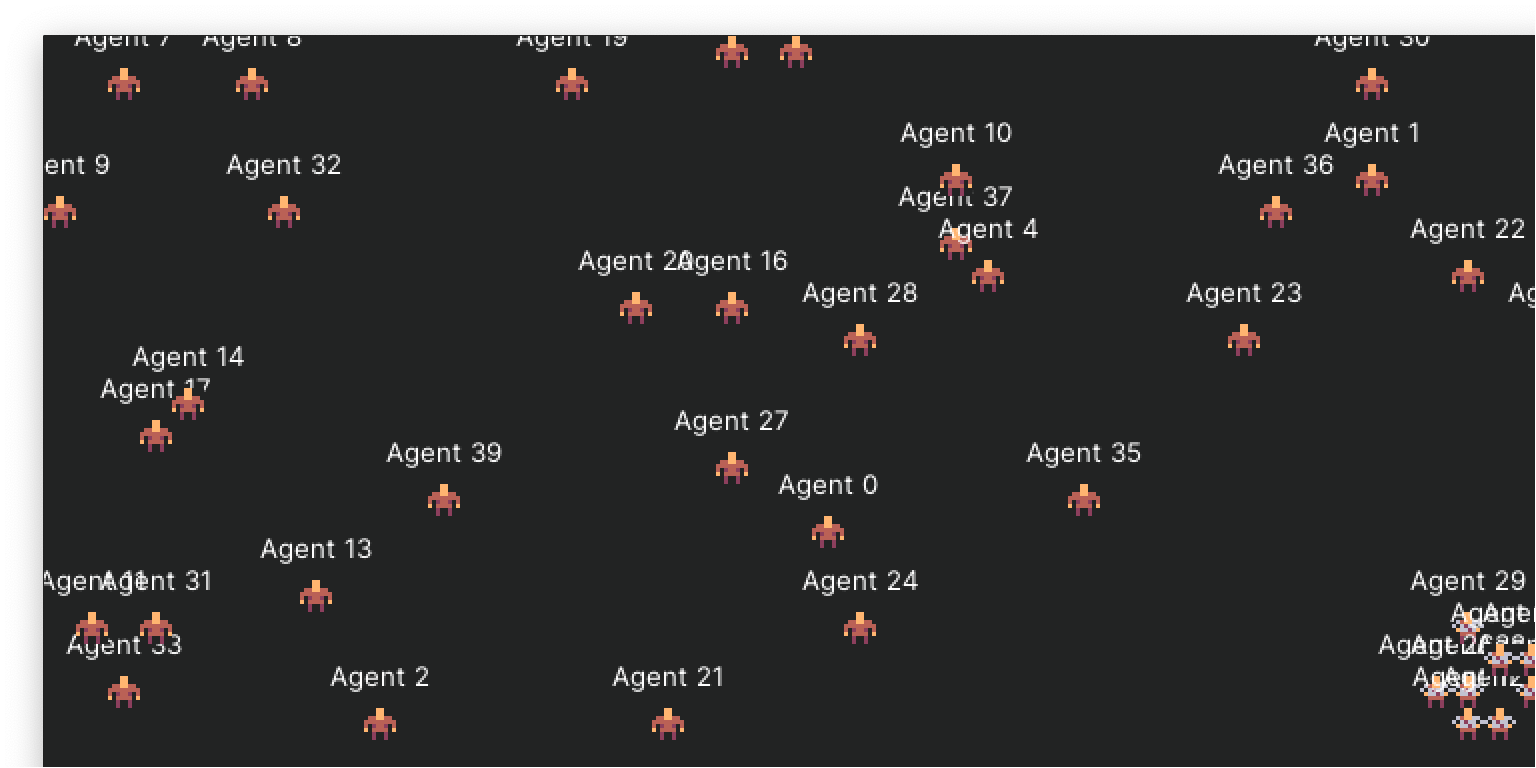
\includegraphics[width=0.3\textwidth]{images/chapter2/sir1/sir_33.png}\label{fig:images/chapter2/sir1/sir_33.png}}
    \hspace*{\fill}
    \subfigure[Step 128]{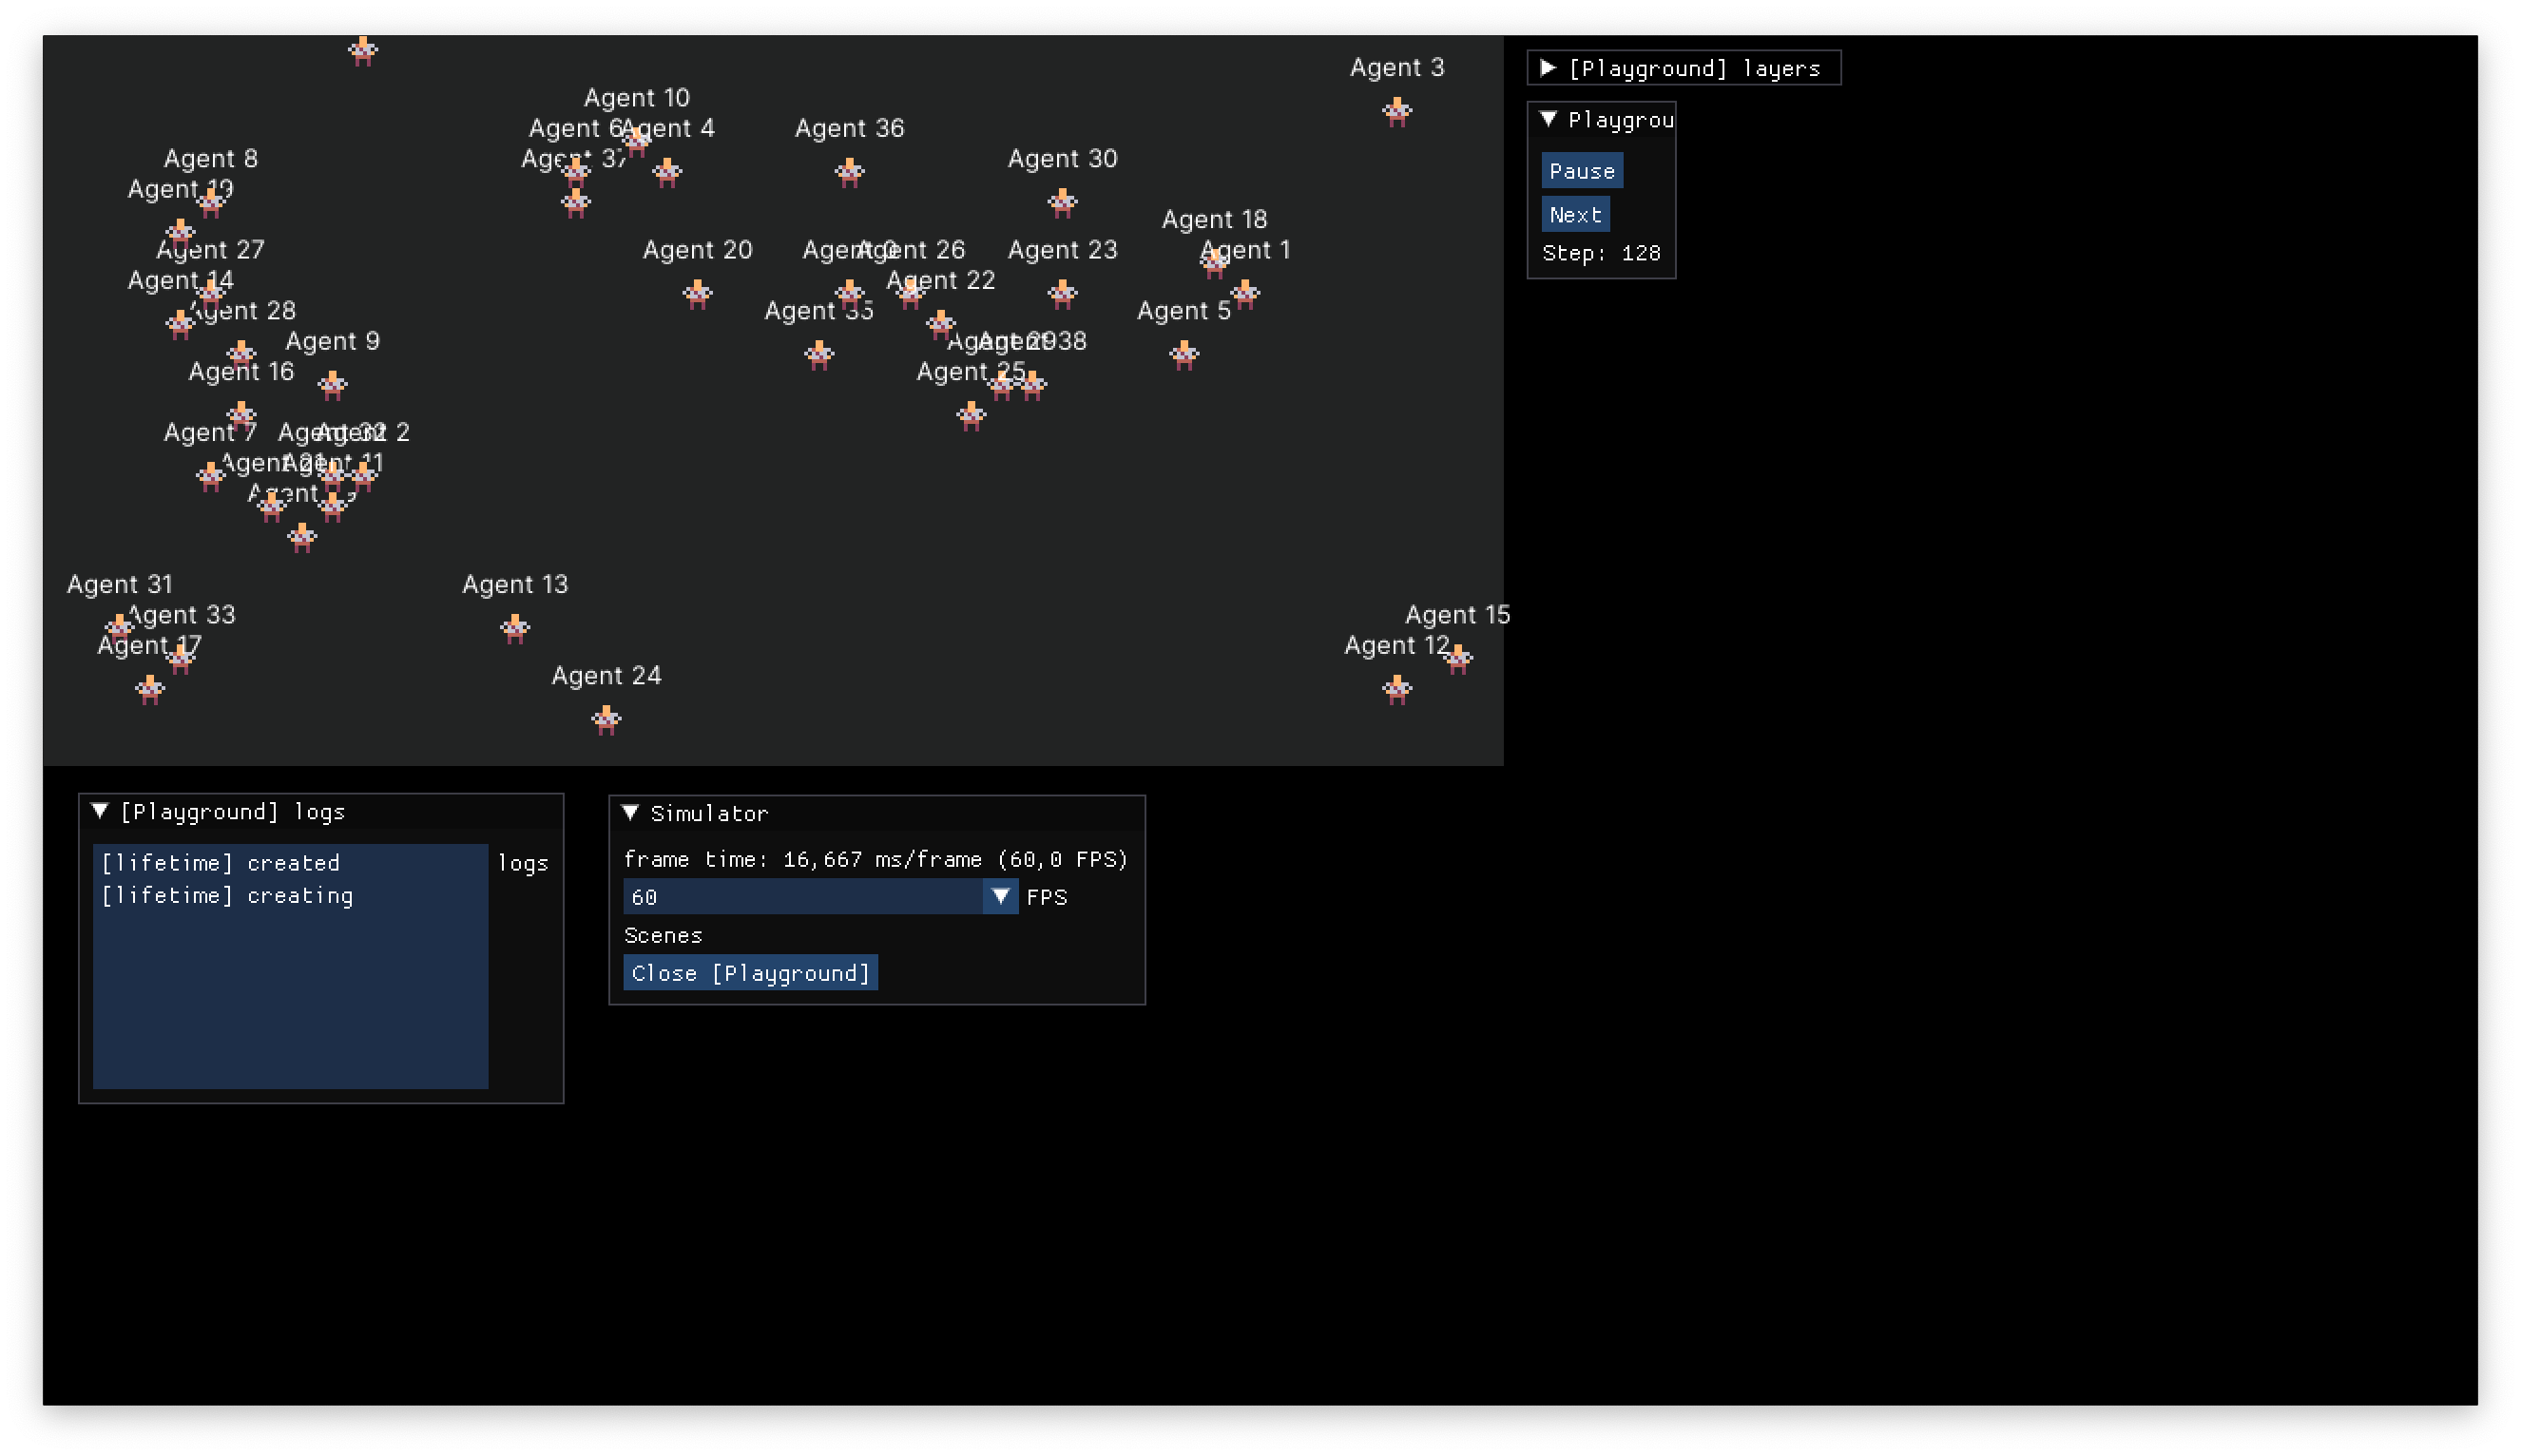
\includegraphics[width=0.3\textwidth]{images/chapter2/sir1/sir_128.png}\label{fig:images/chapter2/sir1/sir_123.png}}

    \caption{Experiment 2} \label{fig:experiment1}
\end{figure}

It is worth noting that because the $\gamma$ parameter was set to zero, no agents could recover from being infected and so the equations were simplified to the following.

\begin{equation} \label{eq:sir1_gamma0}
    \frac{{dS}}{{dt}} = -\frac{{\beta \cdot S \cdot I}}{{N}}
\end{equation}

\begin{equation} \label{eq:sir2_gamma0}
    \frac{{dI}}{{dt}} = \frac{{\beta \cdot S \cdot I}}{{N}}
\end{equation}

\begin{equation} \label{eq:sir3_gamma0}
    \frac{{dR}}{{dt}} = 0
\end{equation}

One can easily see that now:

\begin{equation}
    \frac{{dI}}{{dt}} = -\frac{{dS}}{{dt}}
\end{equation}

\subsection{Experiment 3 - surviving agents}

In reality the recovery rate is seldom going to be zero, even in terms of information propagation.
People receive new information every day and even the most interesting news become old and outdated quickly.
In terms of information propagation an agent becoming removed from the simulation signifies that they grew bored of the information or that it became outdated and thus that particular agent is no longer going to participate in spreading it.

% Experiment 3

A rather interesting observation made during testing was that because of the random distribution of agents, when the $\gamma$ parameter was greater than zero, it was often the case that a single individual survived.
Example of this situation is shown on figures \ref{fig:images/chapter2/sir2/sir_1.png}, \ref{fig:images/chapter2/sir2/sir_53.png} and \ref{fig:images/chapter2/sir2/sir_123.png}.
In this particular example the agents' lifetime upon infection became limited to just 24 simulation steps.
The population size change in time is shown on figure \ref{fig:images/chapter2/sir2/sir.png}.

% \begin{figure}[H]
%     \centering
%     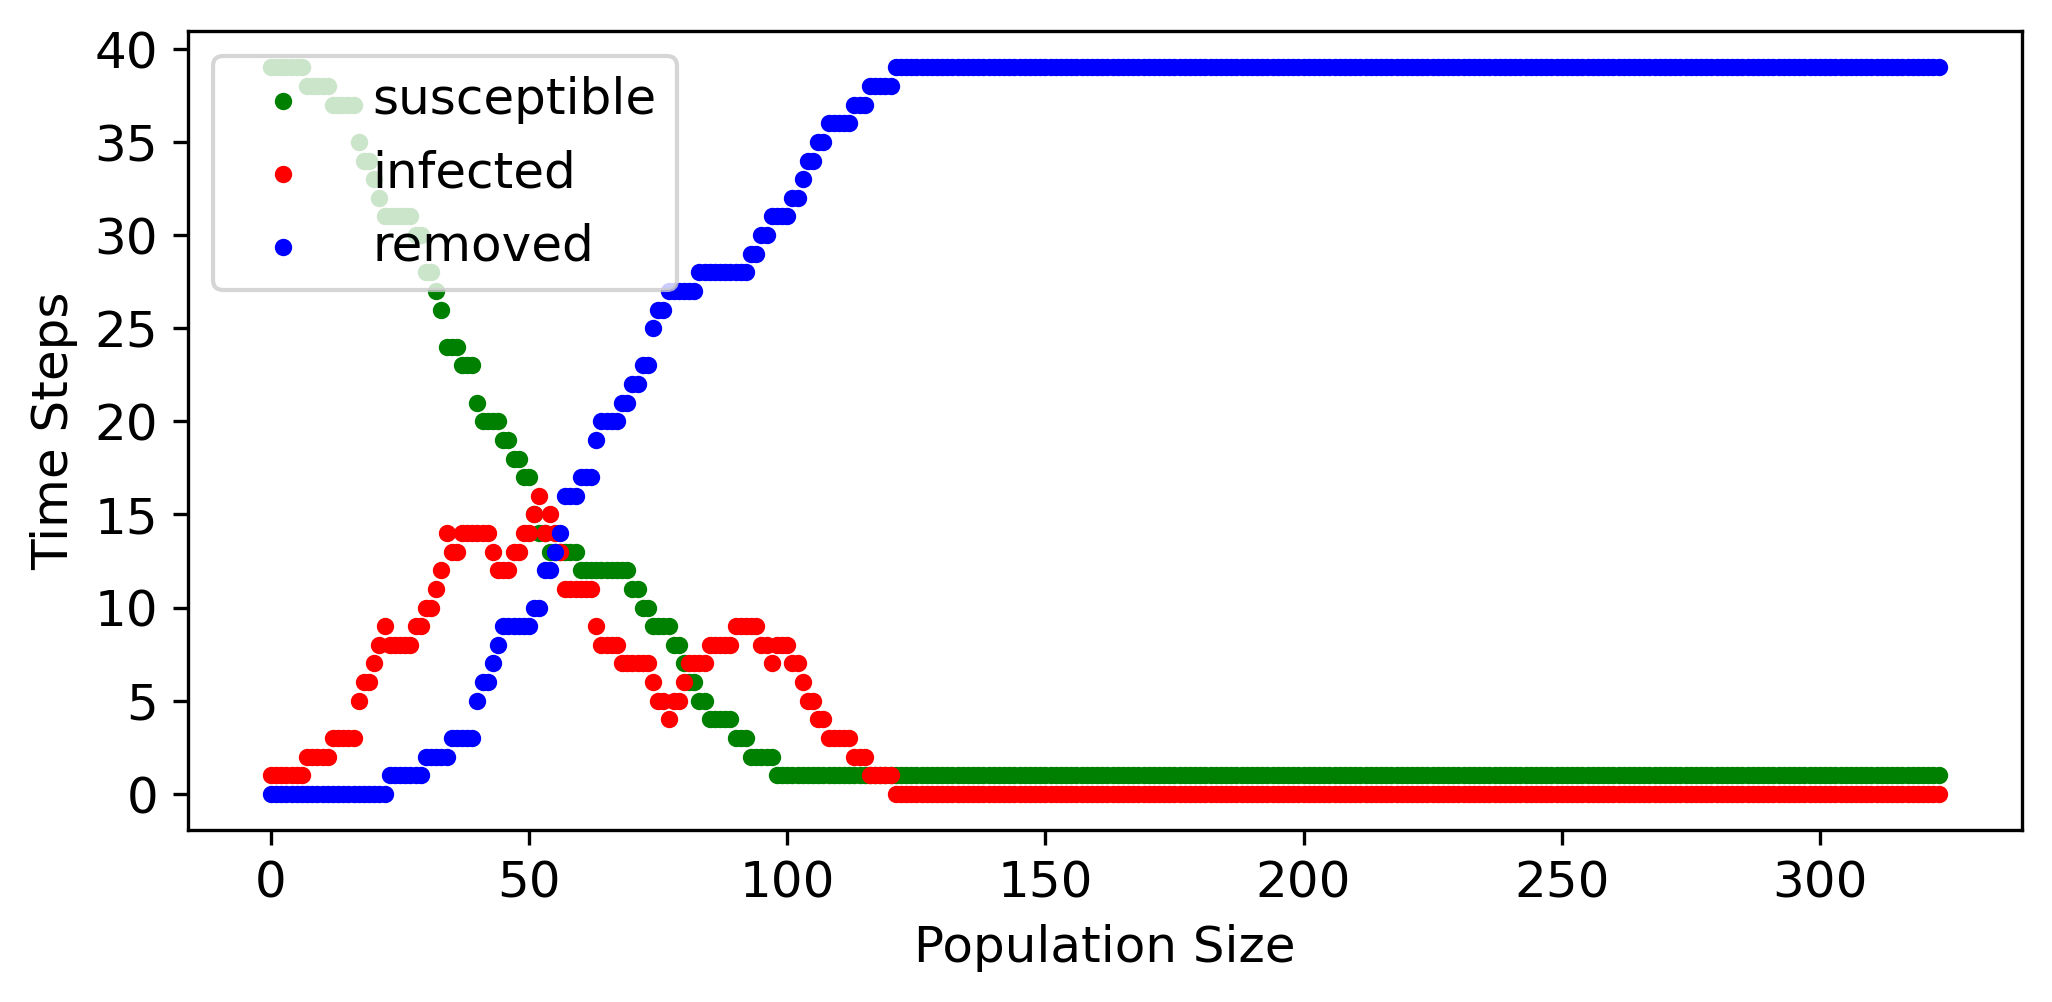
\includegraphics[width=1.0\textwidth]{images/chapter2/sir2/sir.png}
%     \caption{Experiment 3 - SIR}\label{fig:images/chapter2/sir2/sir.png}
% \end{figure}

\begin{figure}[H]
    \centering
    \subfigure[Step 1]{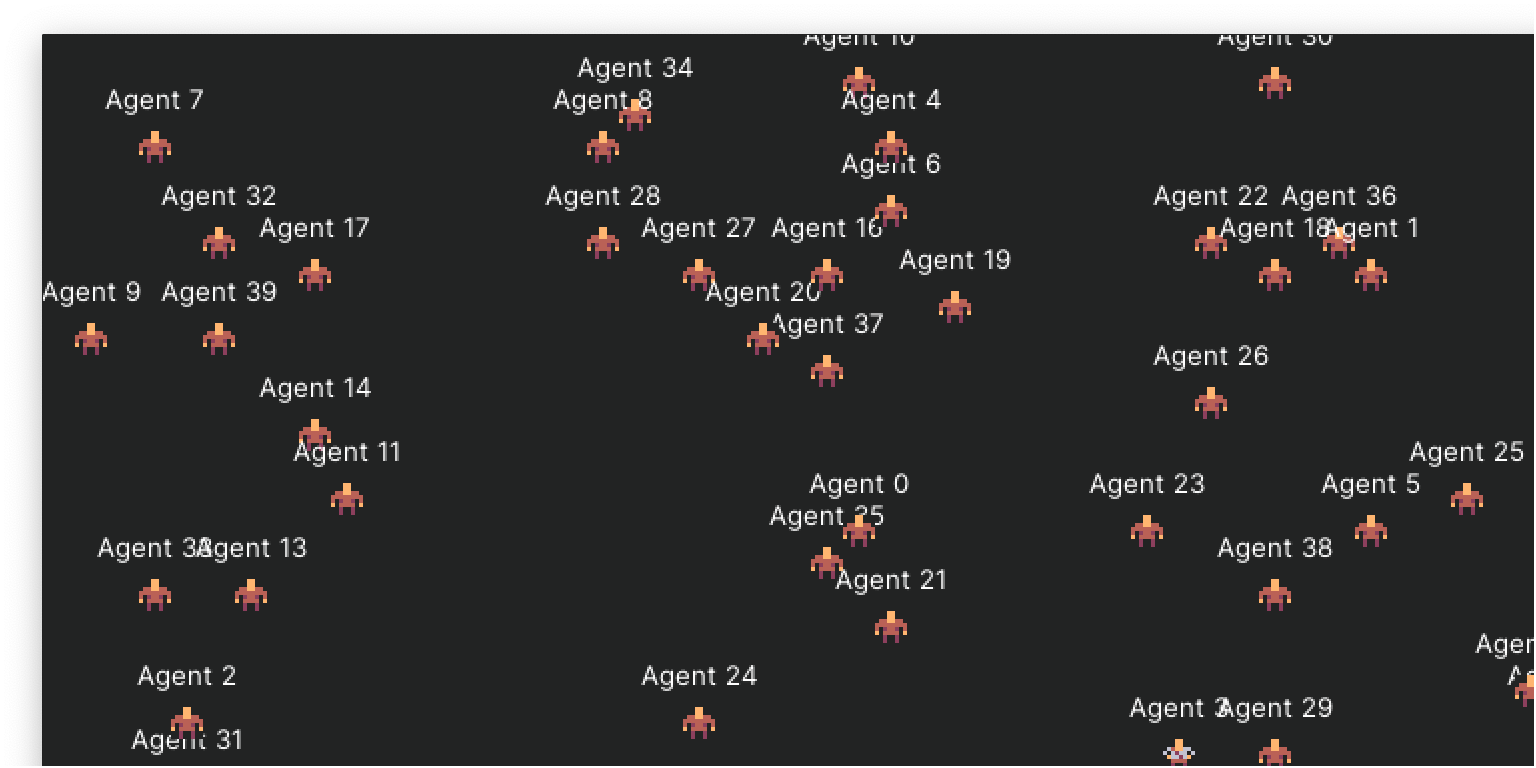
\includegraphics[width=0.3\textwidth]{images/chapter2/sir2/sir_1.png}\label{fig:images/chapter2/sir2/sir_1.png}}
    \hspace*{\fill}
    \subfigure[Step 53]{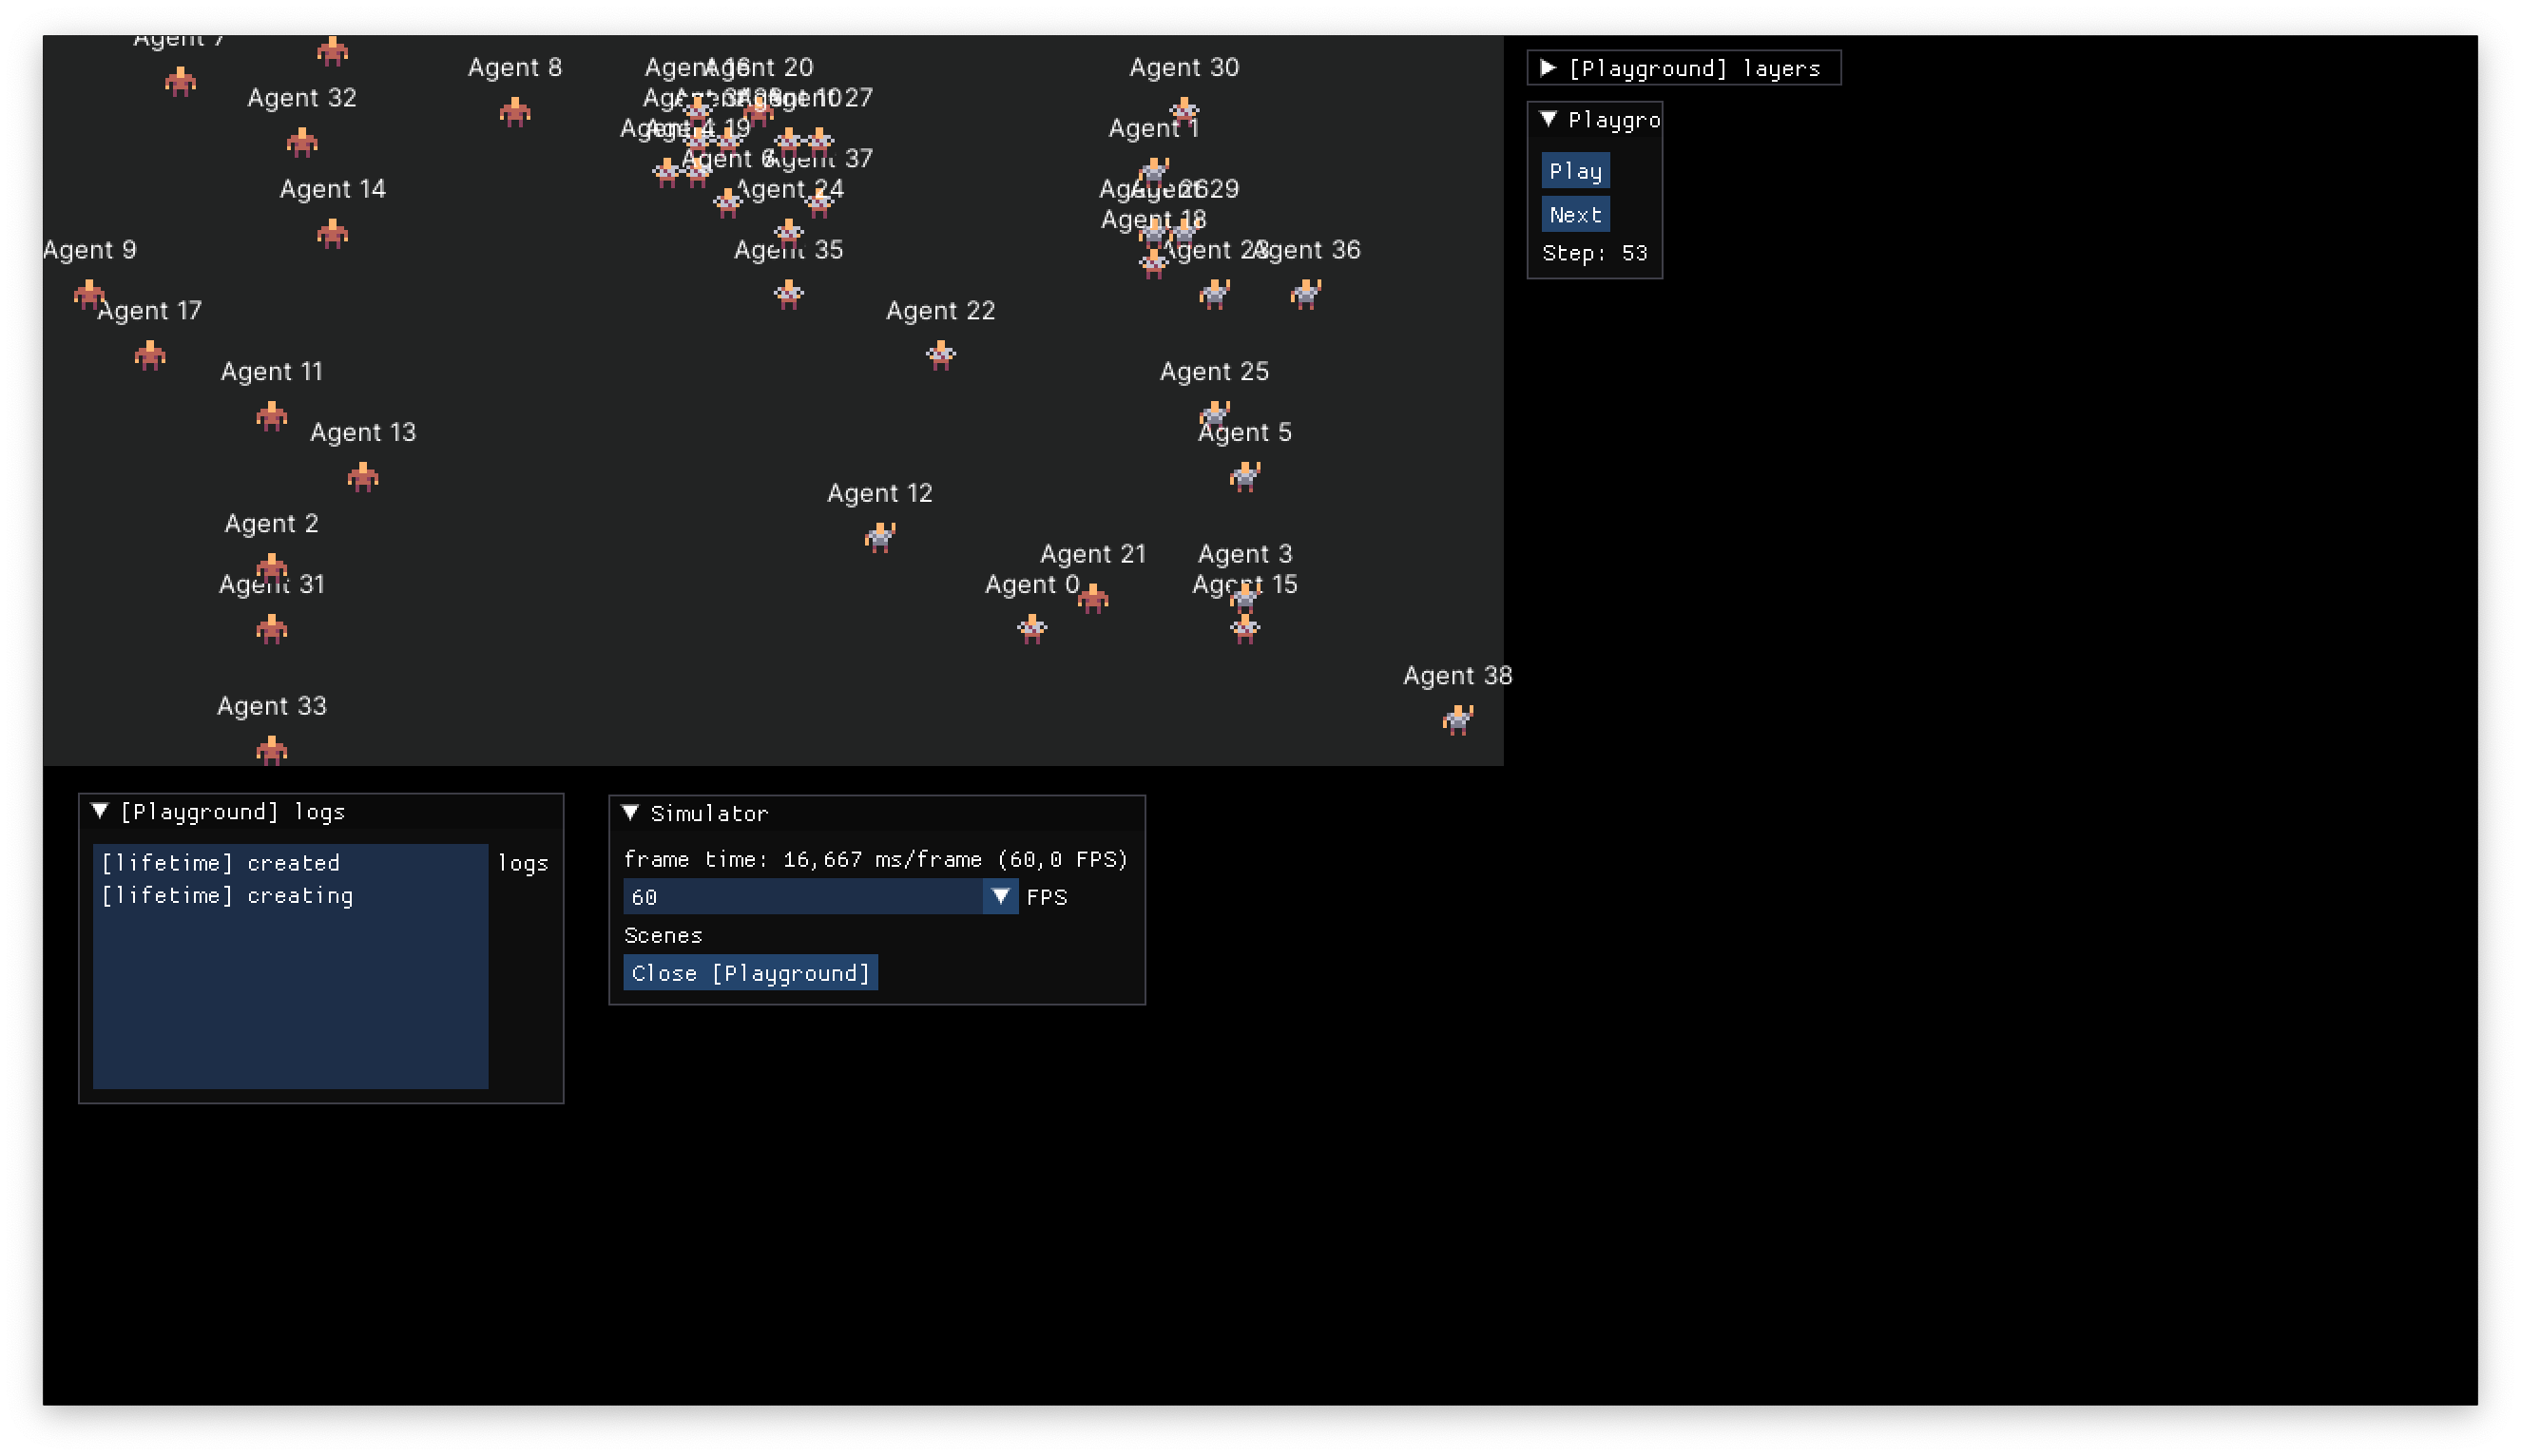
\includegraphics[width=0.3\textwidth]{images/chapter2/sir2/sir_53.png}\label{fig:images/chapter2/sir2/sir_53.png}}
    \hspace*{\fill}
    \subfigure[Step 324]{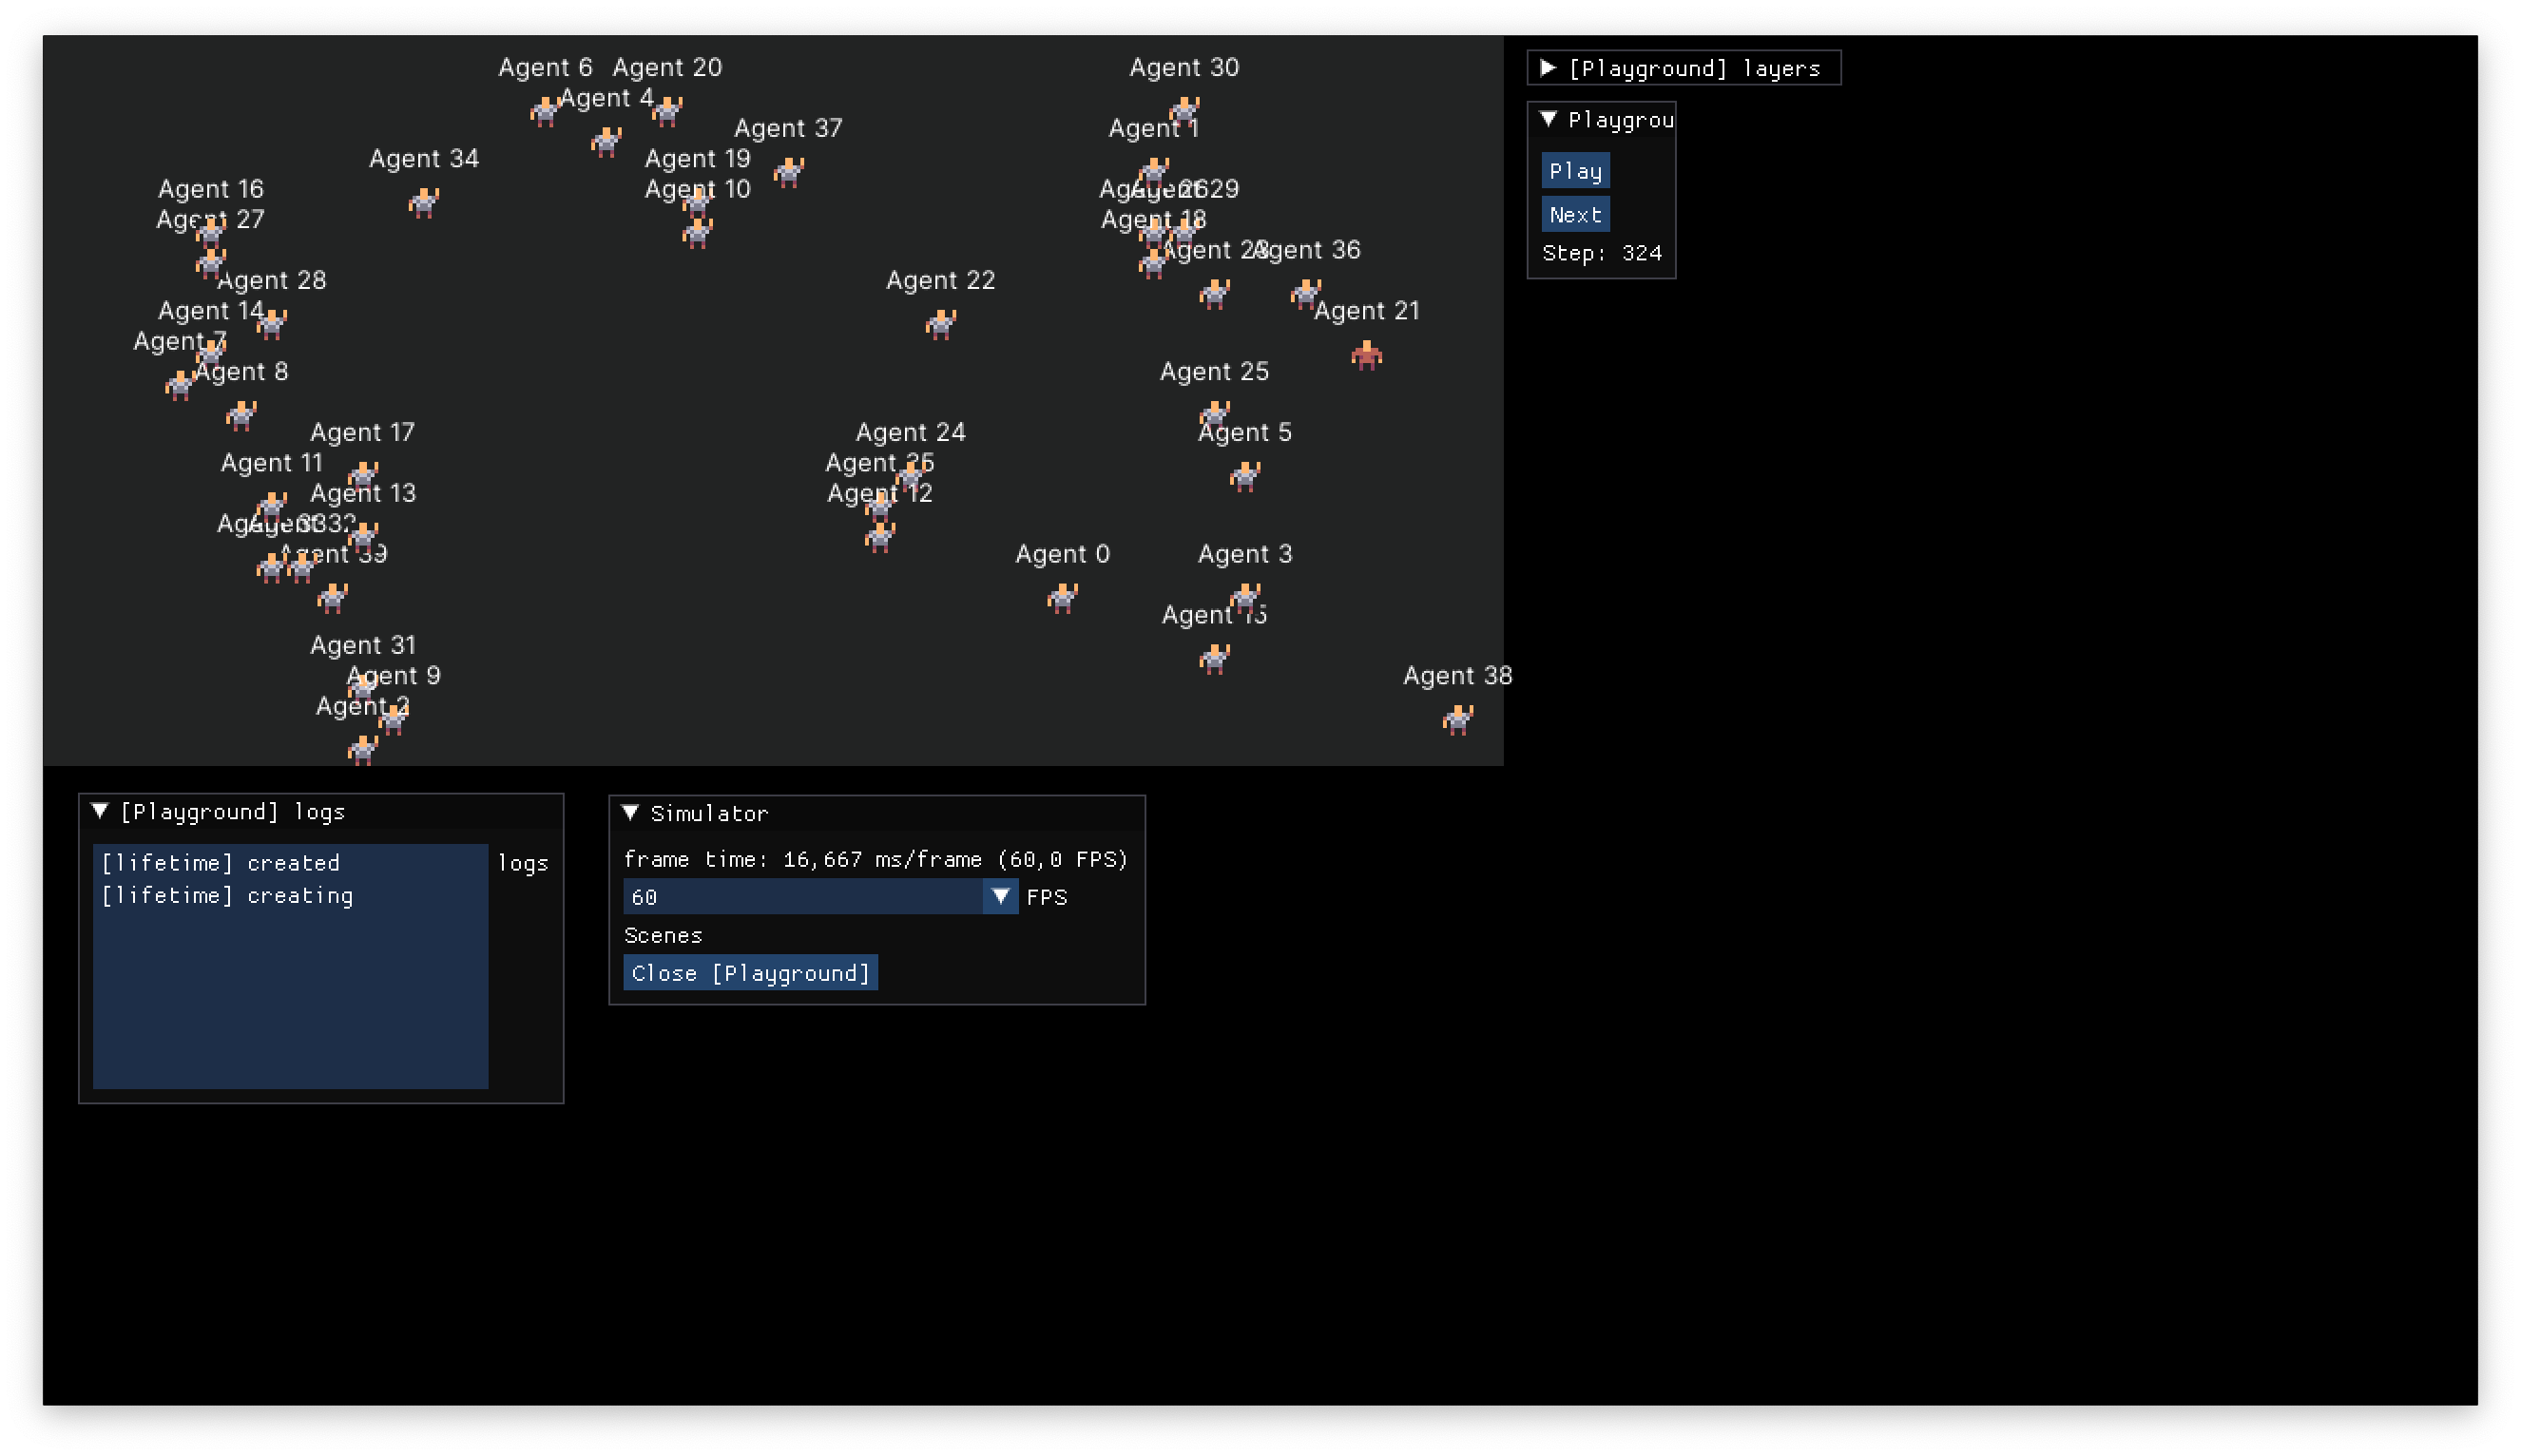
\includegraphics[width=0.3\textwidth]{images/chapter2/sir2/sir_324.png}\label{fig:images/chapter2/sir2/sir_123.png}}

    \caption{Experiment 3} \label{fig:experiment2}
\end{figure}

\subsection{Experiment 4 - stable infection rate}

Normally the recovery rate $\gamma$ is high enough that a disease does not overwhelm the whole population.
The next experiment shows an example of a simulation where infection rate is balanced with the recovery rate such that the number of infected individuals is on roughly the same level.

% Experiment 4

\begin{figure}[H]
    \centering
    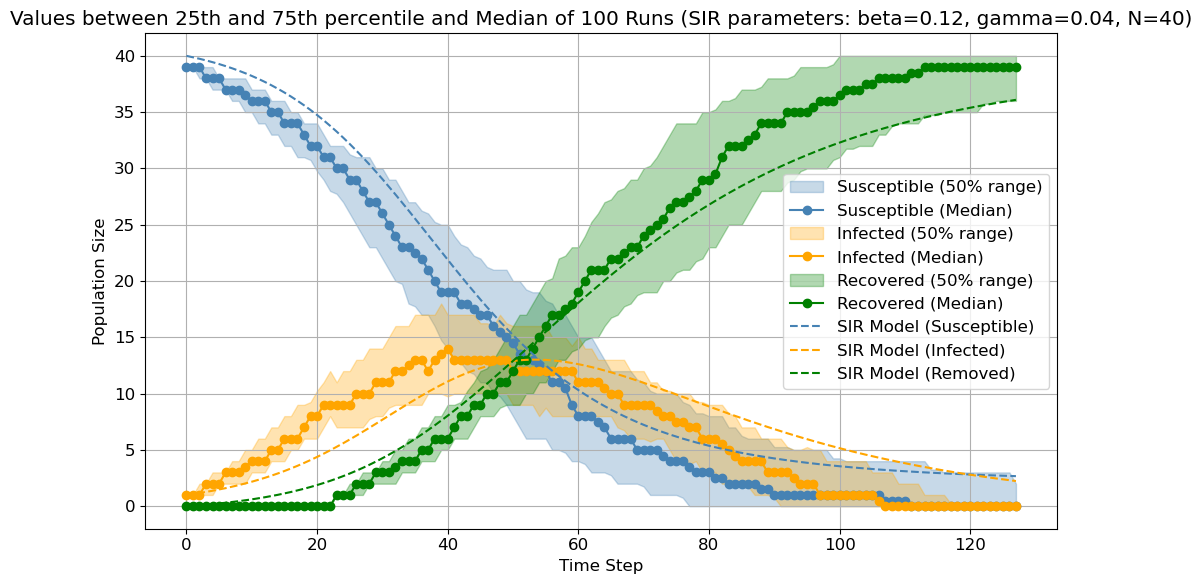
\includegraphics[width=1.0\textwidth]{images/chapter2/experiment3.png}
    \caption{Experiment 4 - population size over time}\label{fig:images/chapter2/experiment3.png}
\end{figure}

% \begin{figure}[H]
%     \centering
%     \subfigure[Experiment]{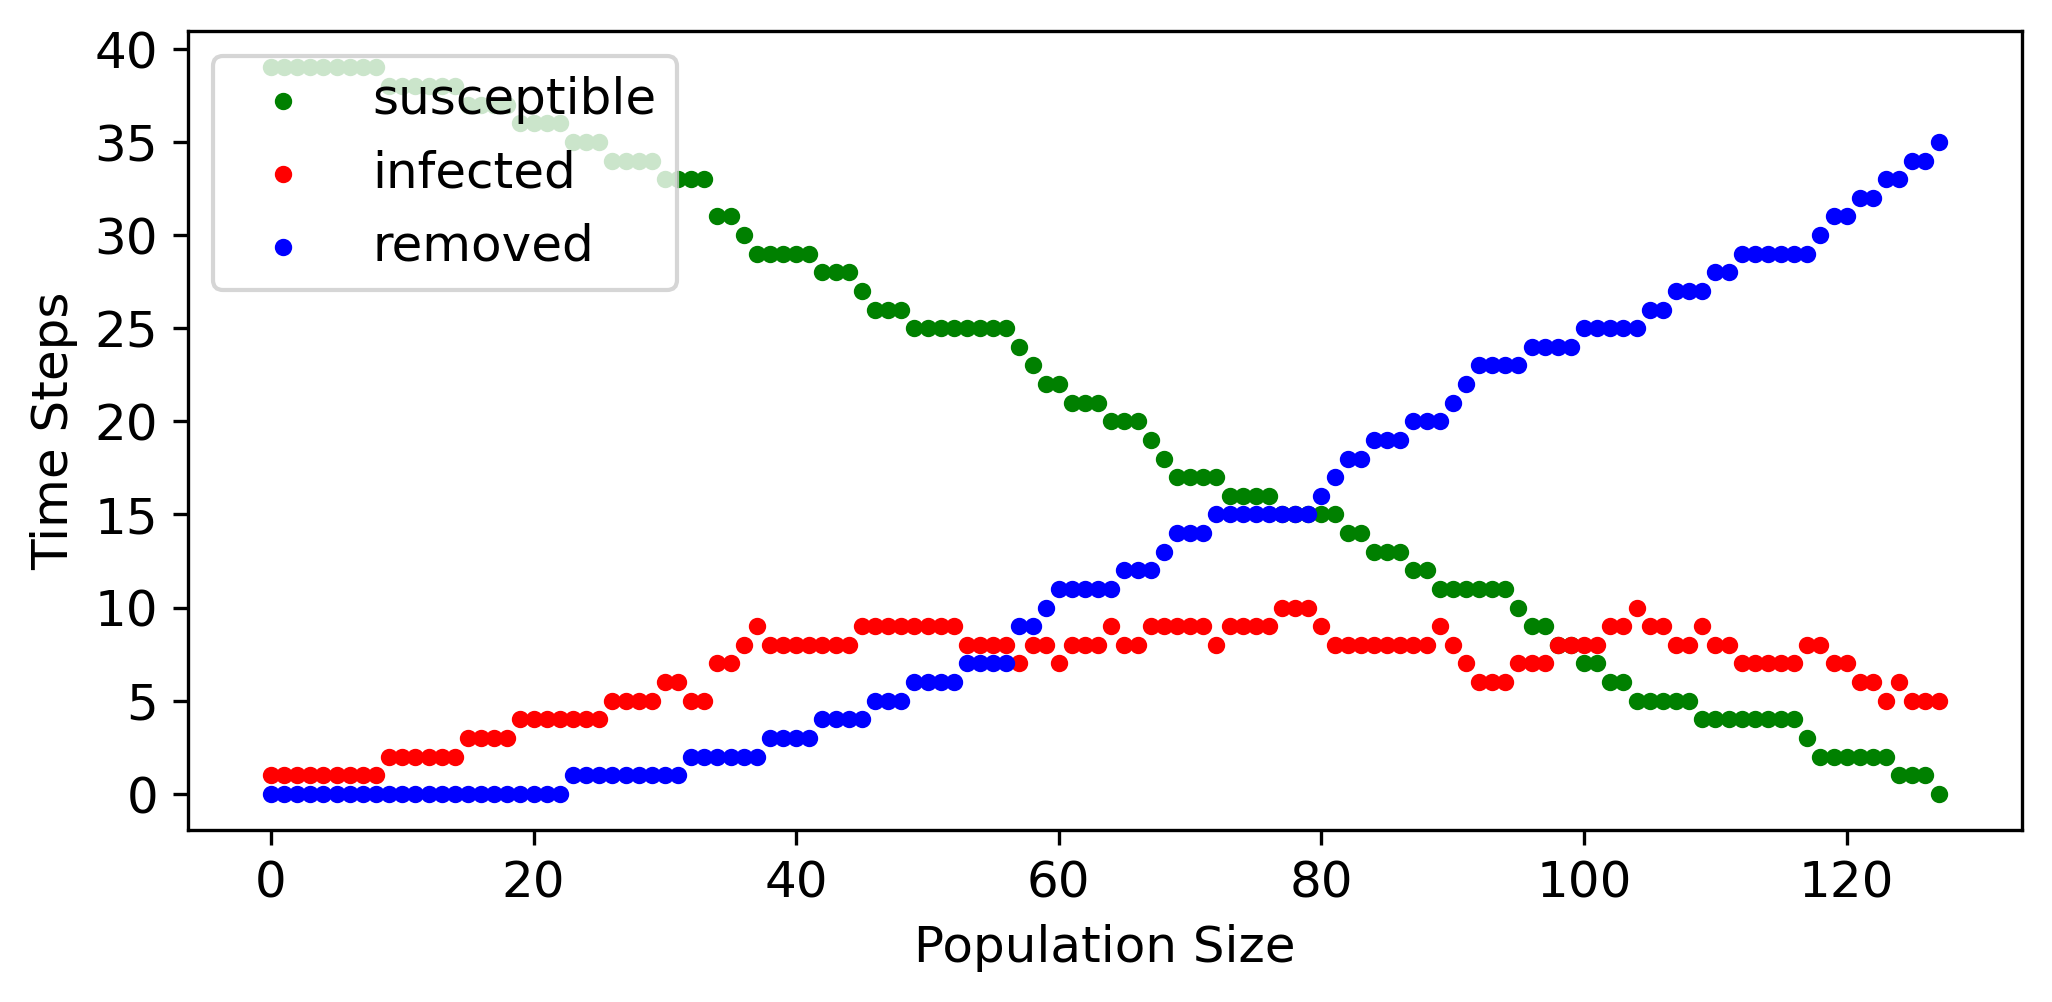
\includegraphics[width=0.48\textwidth]{images/chapter2/sir3/sir.png}\label{fig:images/chapter2/sir3/sir.png}}
%     \hspace*{\fill}
%     \subfigure[$\beta = 0.03, \gamma = 0.01, N = 40$]{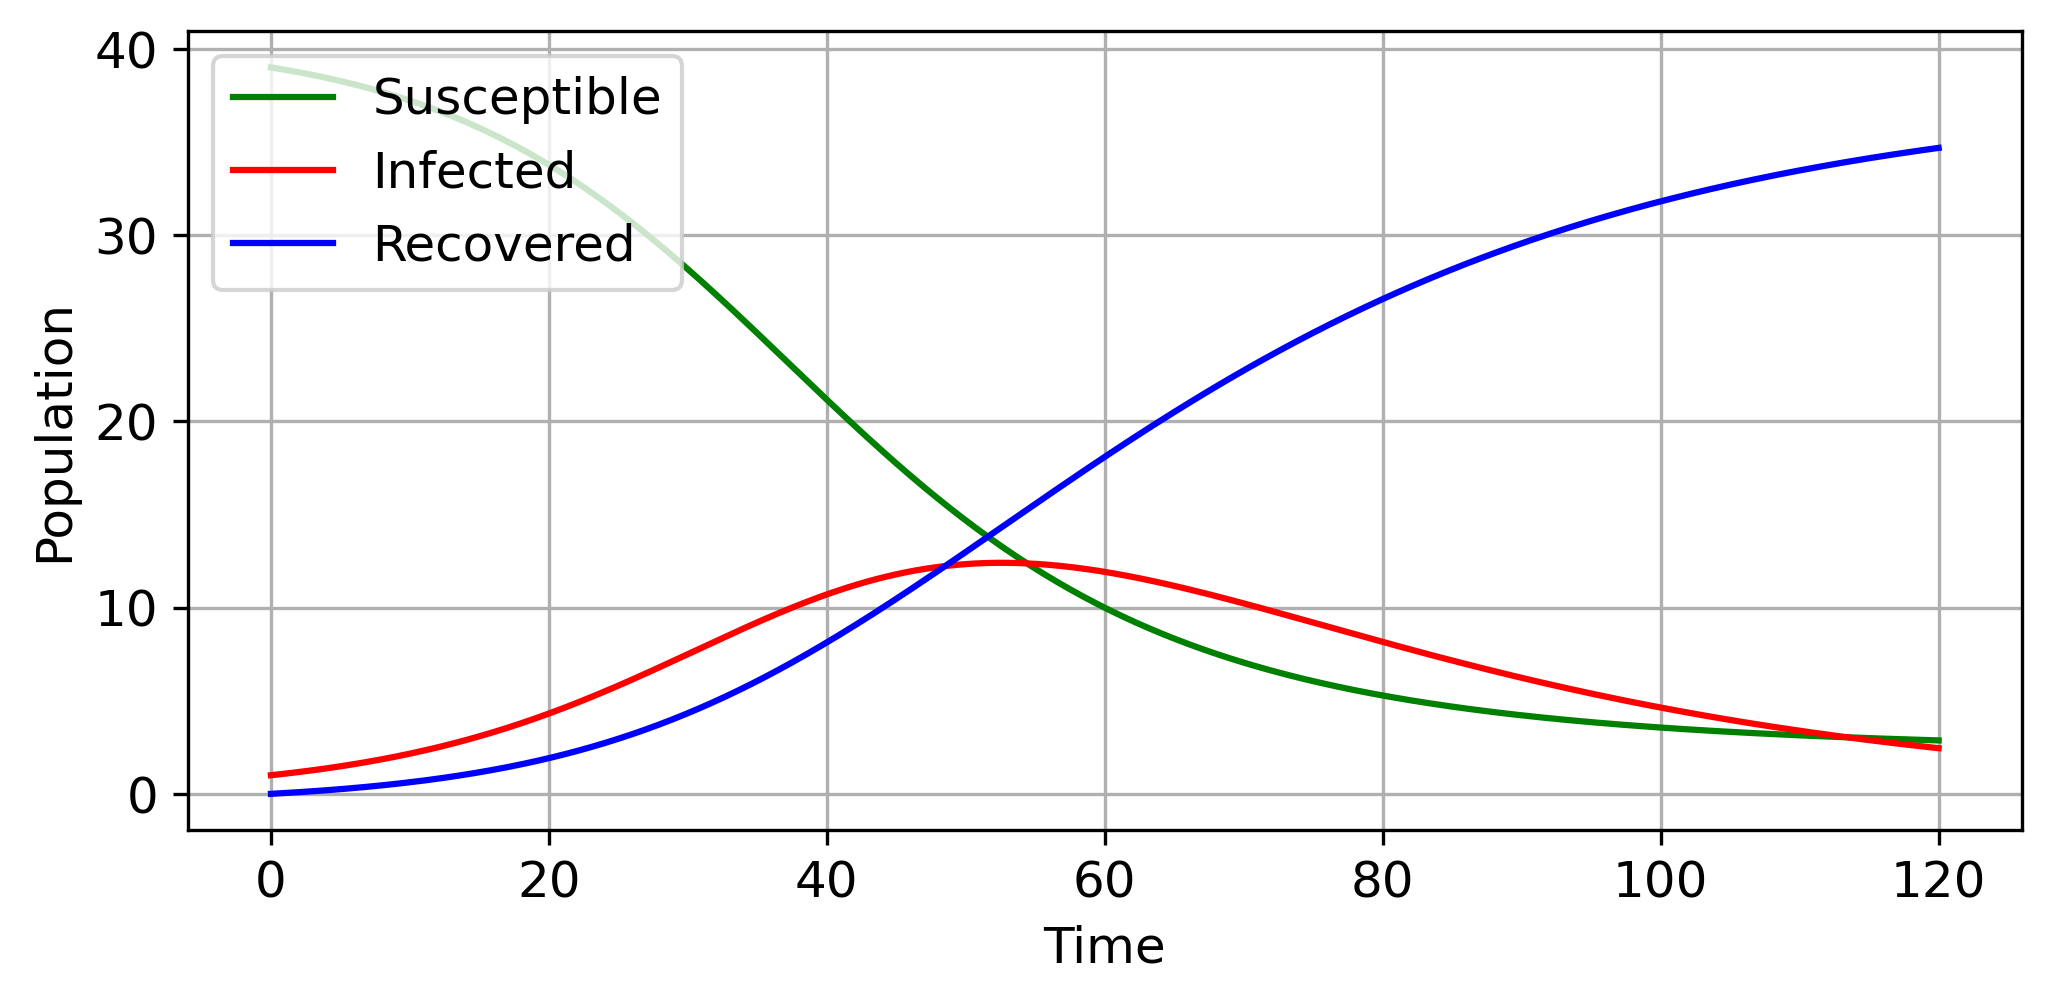
\includegraphics[width=0.48\textwidth]{images/chapter2/sir_ref/sir_2.png}\label{fig:images/chapter2/sir_ref/sir_2.png}}
%     \caption{Experiment 4 - SIR vs Experiment} \label{fig:experiment4-diagrams}
% \end{figure}

Figure \ref{fig:images/chapter2/experiment3.png} illustrates that the level of infection remains somewhat constant for the whole duration of the simulation.
The corresponding SIR model's parameters for this experiment are $\beta = 0.12, \gamma = 0.04, N = 40$.
% It correlates with the SIR model parameters $\beta = 0.03, \gamma = 0.01, N = 40$ as shown on figure \ref{fig:images/chapter2/experiment3.png}.
Figures \ref{fig:images/chapter2/sir3/sir_1.png}, \ref{fig:images/chapter2/sir3/sir_79.png} and \ref{fig:images/chapter2/sir3/sir_128.png} show the progression of the simulation up until the last susceptible individual changes state.

\begin{figure}[H]
    \centering
    \subfigure[Step 1]{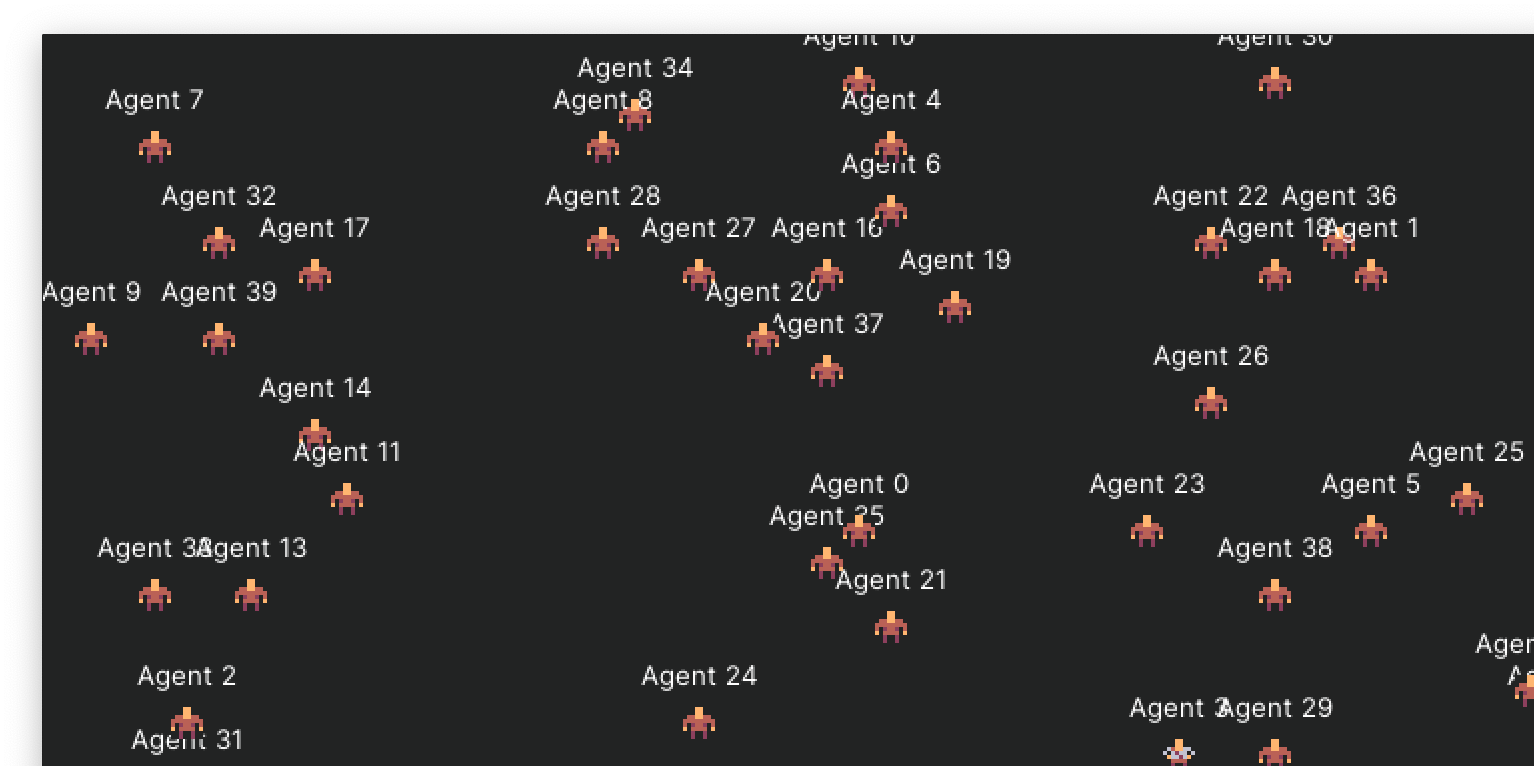
\includegraphics[width=0.3\textwidth]{images/chapter2/sir3/sir_1.png}\label{fig:images/chapter2/sir3/sir_1.png}}
    \hspace*{\fill}
    \subfigure[Step 79]{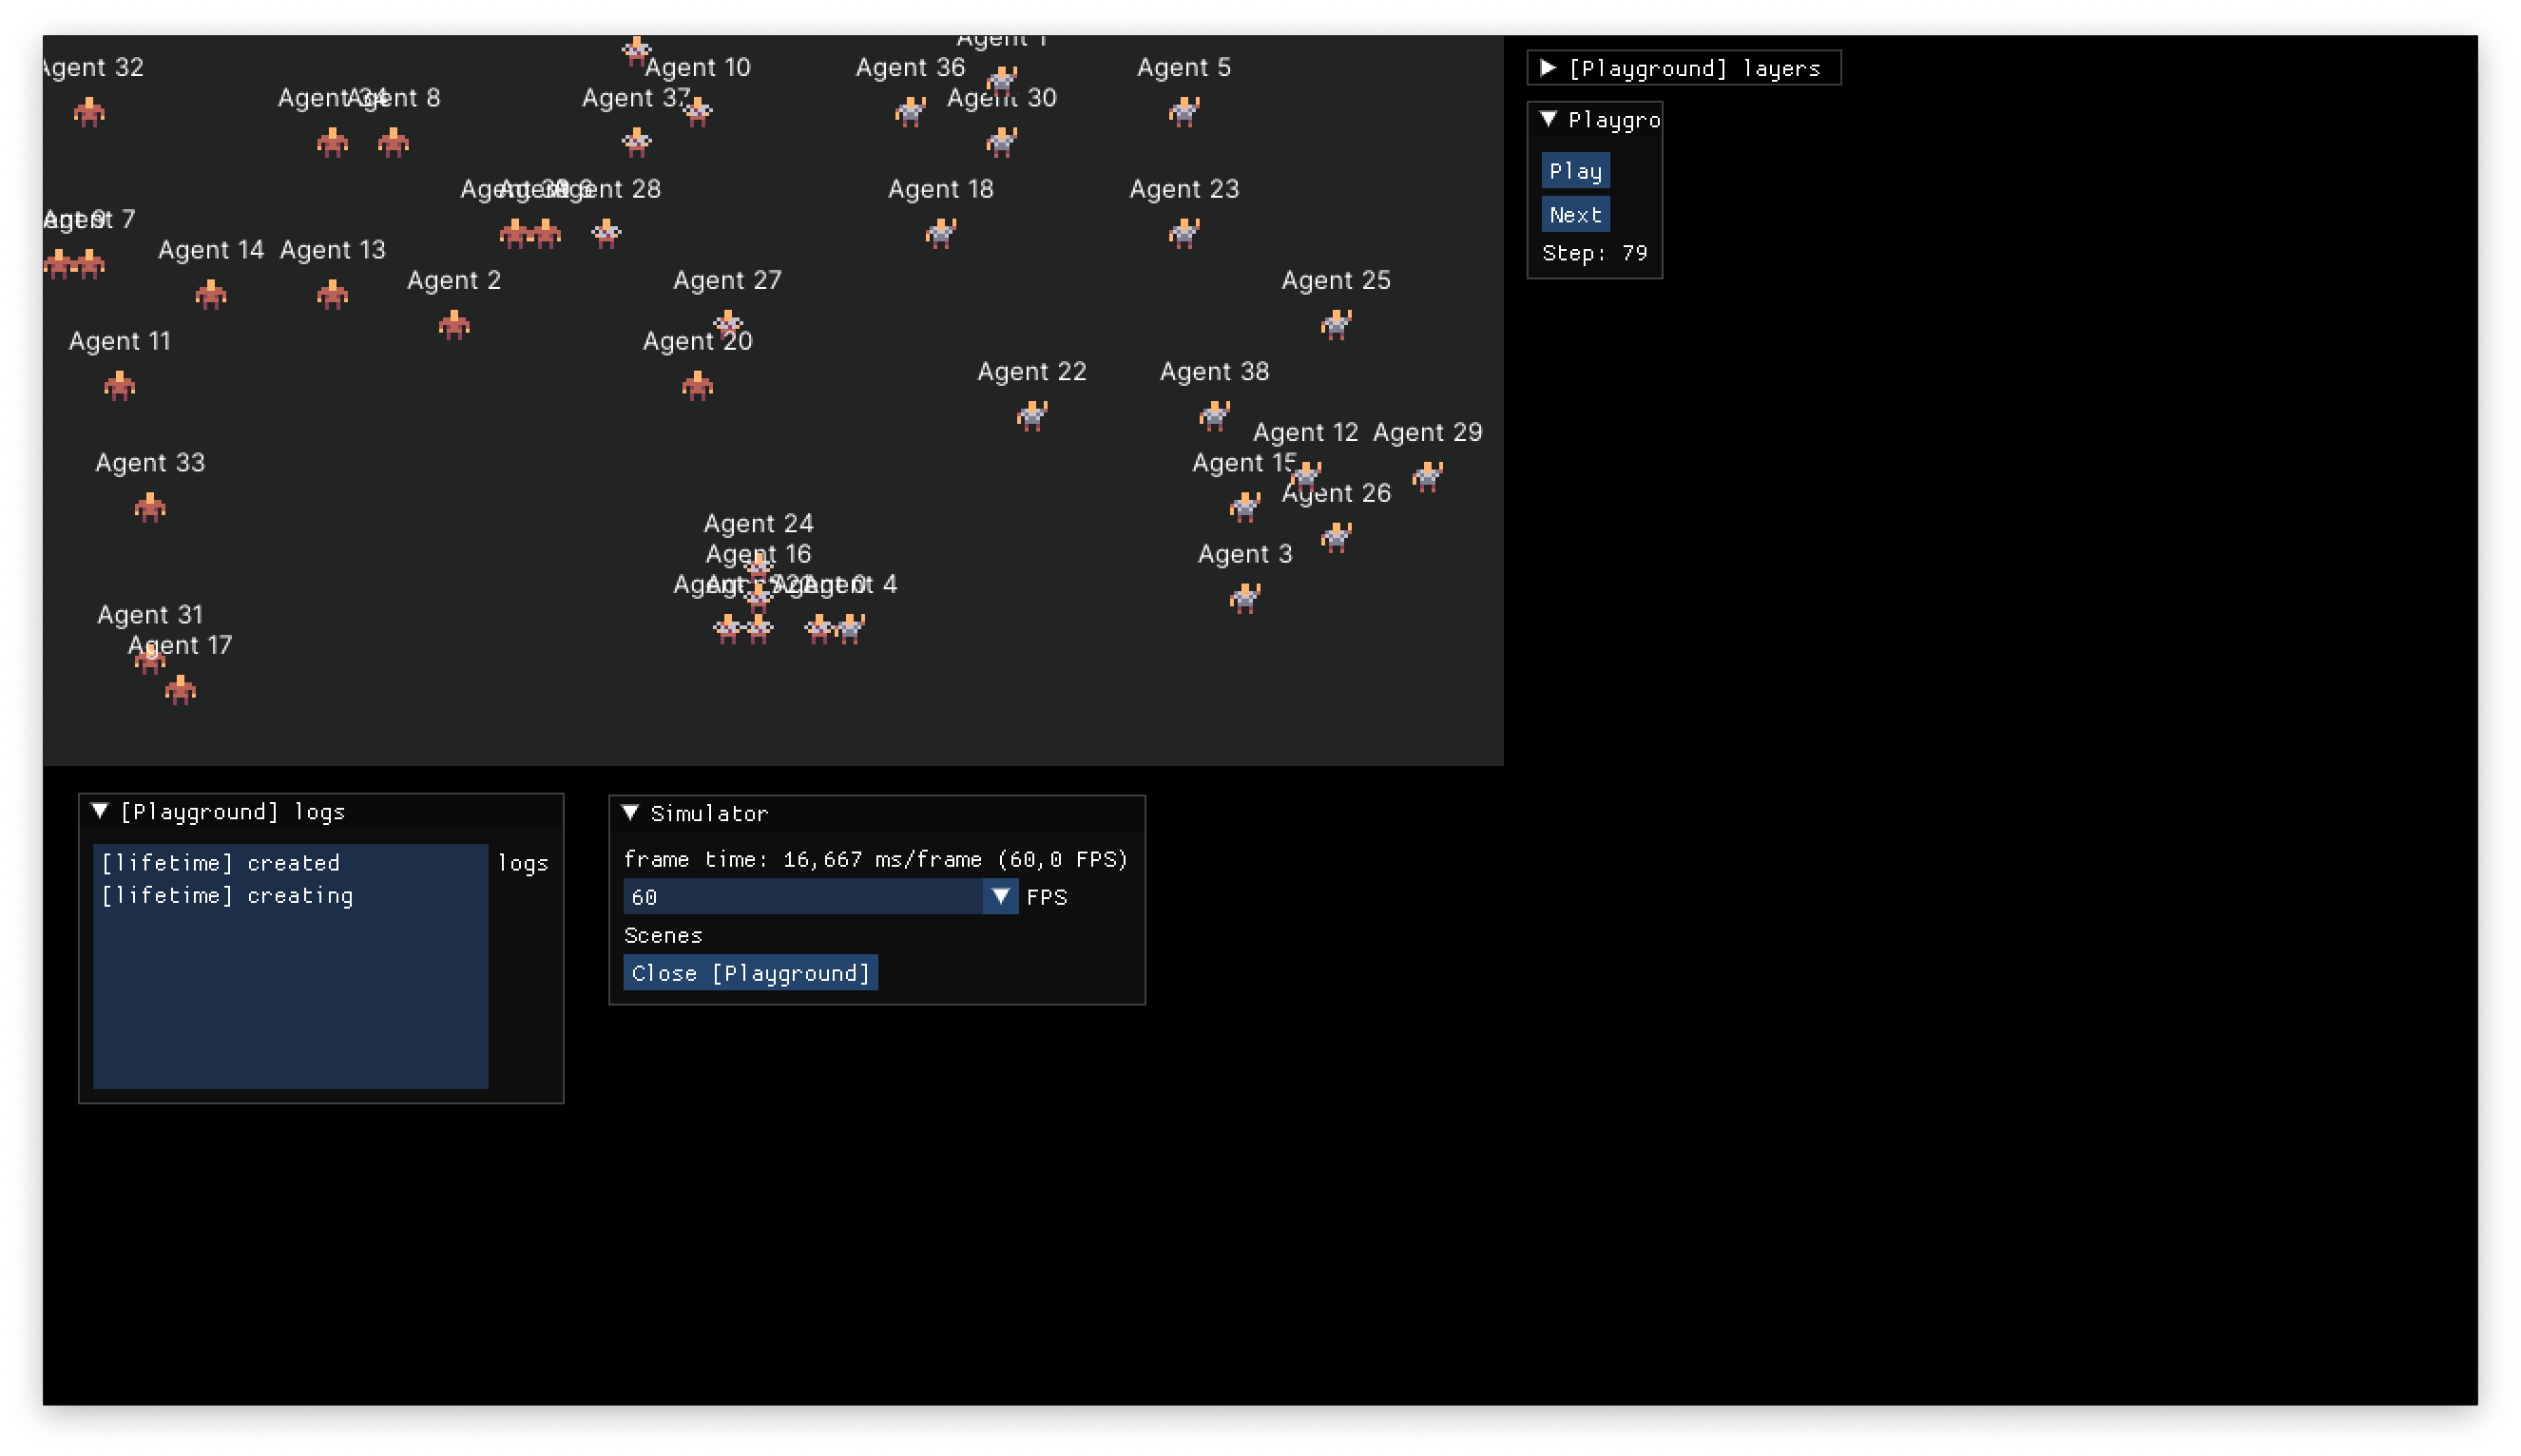
\includegraphics[width=0.3\textwidth]{images/chapter2/sir3/sir_79.png}\label{fig:images/chapter2/sir3/sir_79.png}}
    \hspace*{\fill}
    \subfigure[Step 128]{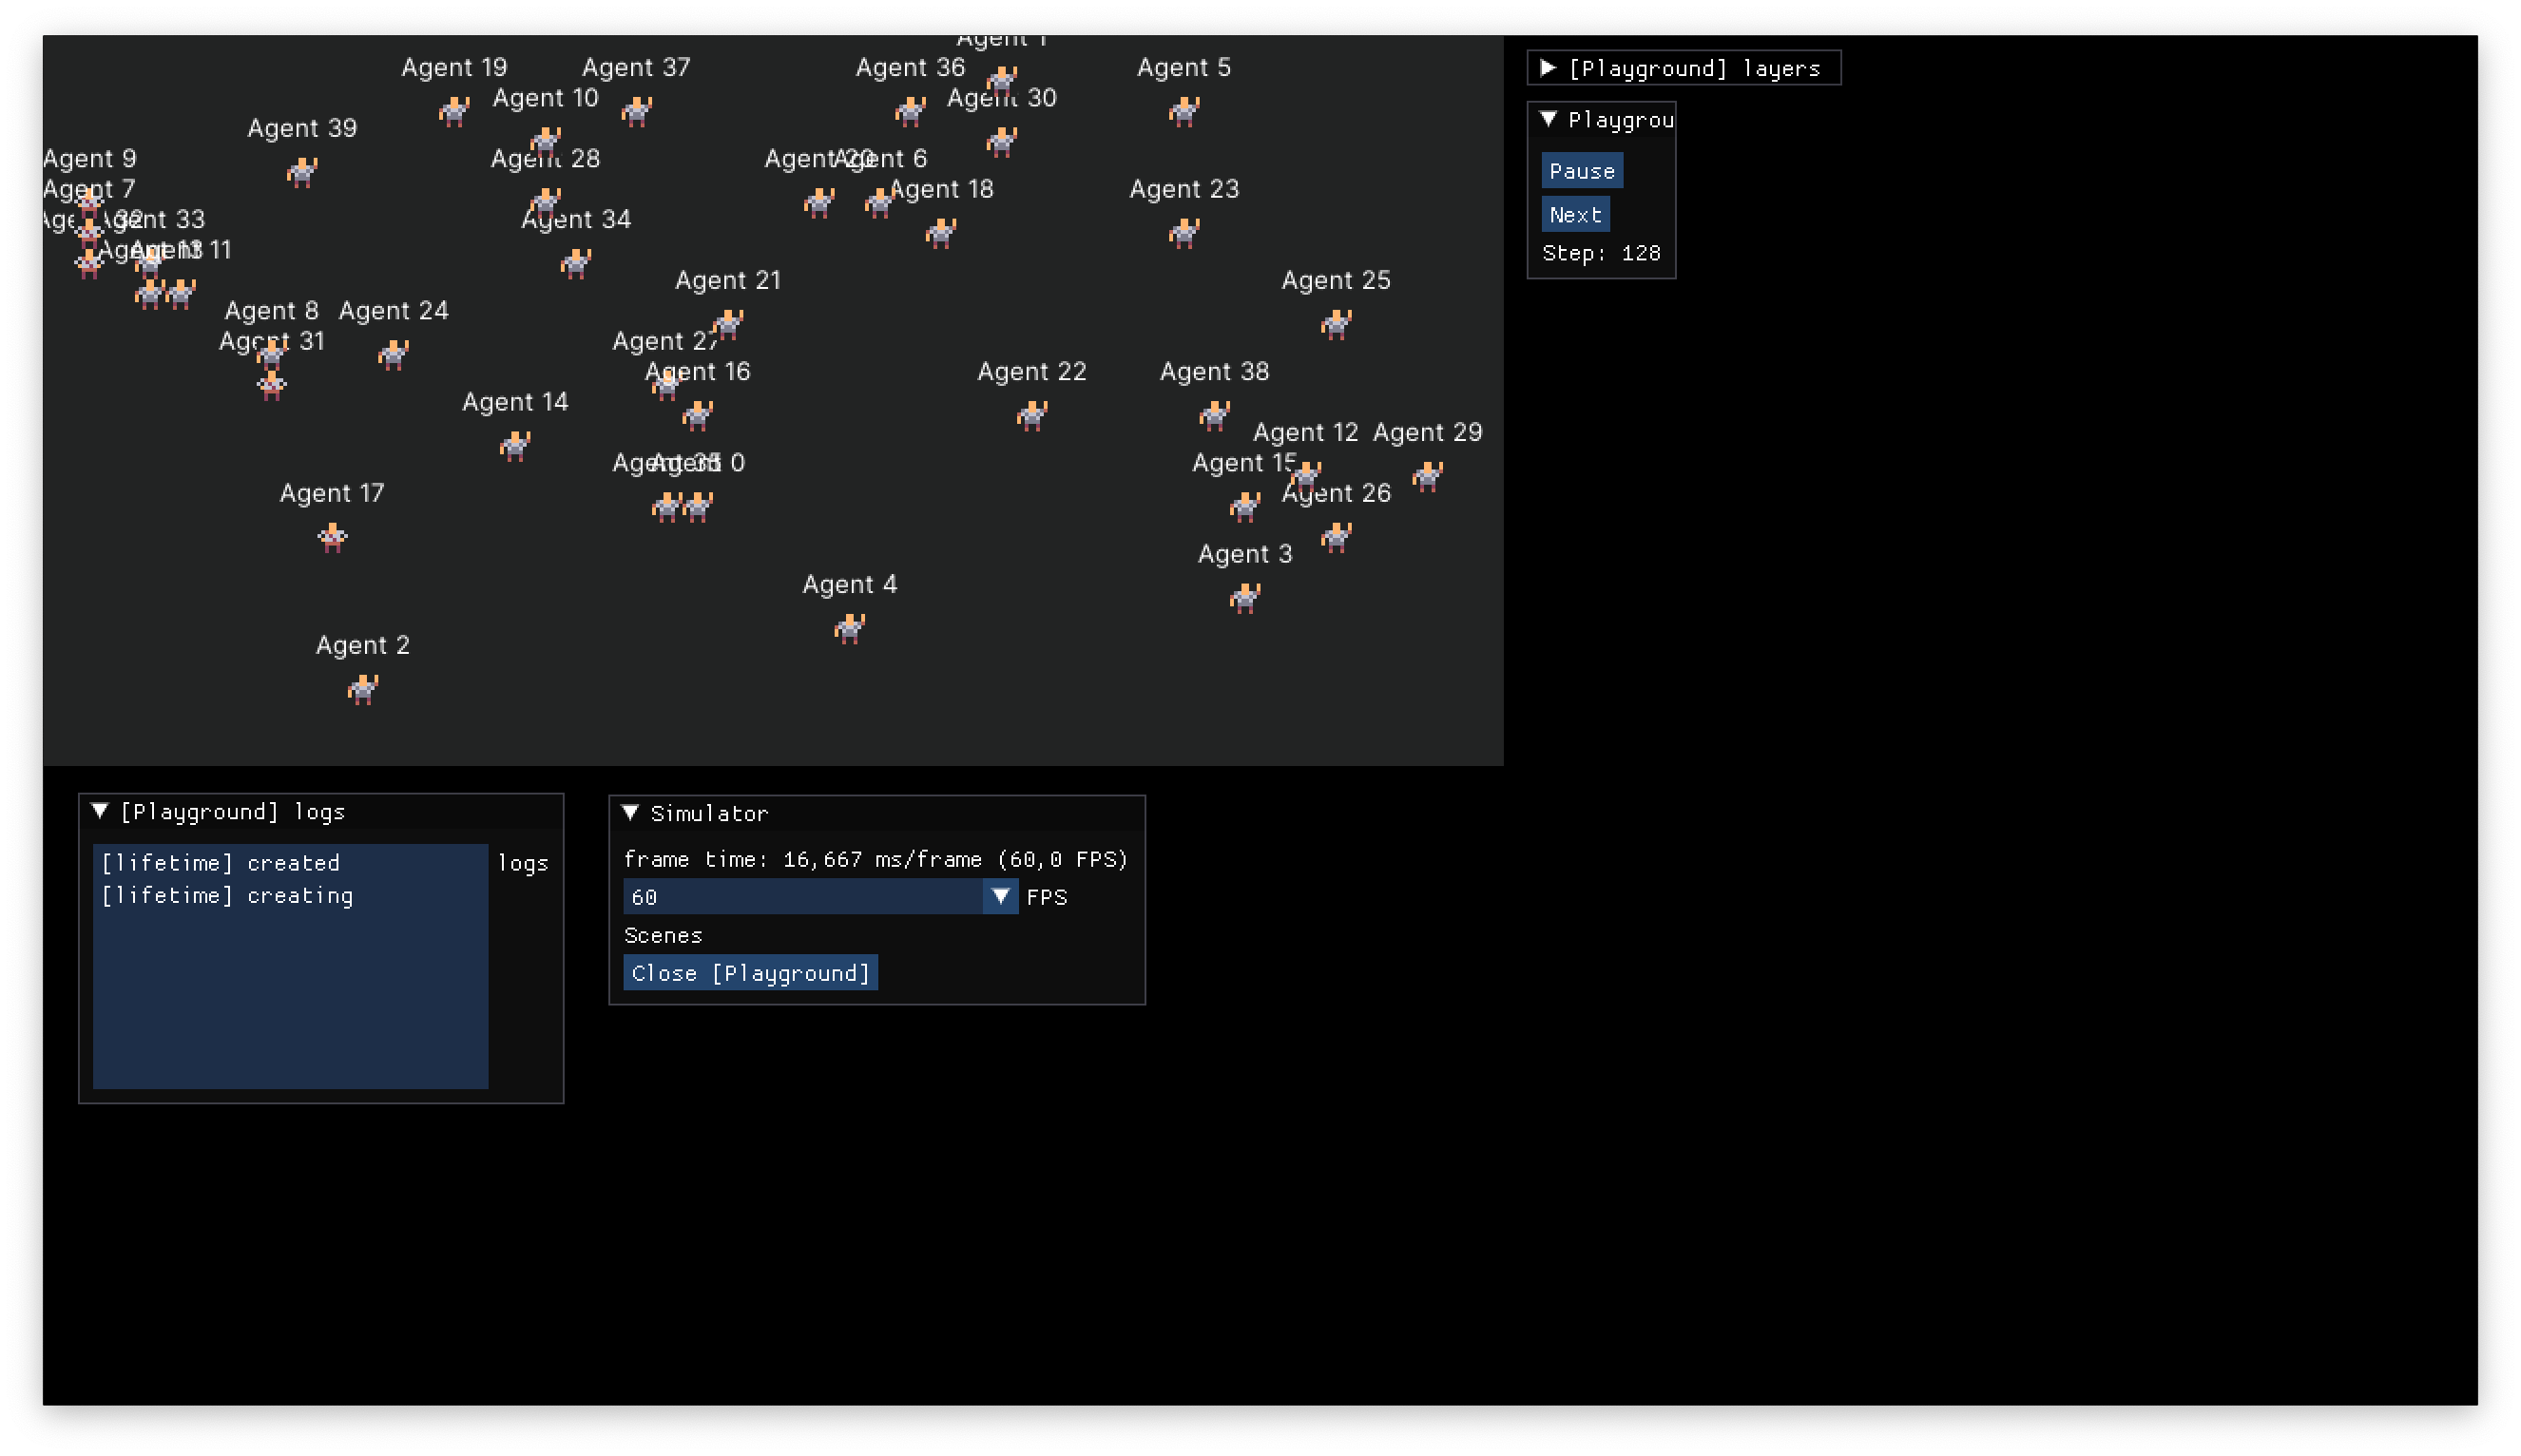
\includegraphics[width=0.3\textwidth]{images/chapter2/sir3/sir_128.png}\label{fig:images/chapter2/sir3/sir_128.png}}

    \caption{Experiment 4} \label{fig:experiment3}
\end{figure}

\subsection{Experiment 5 - analysis of population density influence}

In order to determine whether the solution is capable of scaling up to simulate bigger and more complex game worlds, the fifth experiment was conducted.
Four population sizes have been chosen for analysis: 16, 32, 64 and 128.
At each population size, three simulations of a hundred runs each were performed.
Each simulation differed in the choice of the lifetime parameter.

The choice of the lifetime parameter as the additional axis of analysis was made due to the assumption that at lower population densities there is a risk that agents may fail to reach another agent before they become removed from the simulation.
Results of the experiment are presented on figure \ref{fig:experiment5}.
The initial assumption was proven to be correct as it can be clearly seen that the simulations performed with lifetime parameter set to 8 show a clear change in the simulation dynamics only after the population size became 128.
The combination of population size equal to 128 and the lifetime parameter set to 32 as presented on figure \ref{images/experiments/experiment_128_008_16.png} correlates with a much smaller population size of 16 and lifetime parameter value 16 on figure \ref{images/experiments/experiment_016_016_16.png}.

Subsequent population increases when the lifetime parameter is above a certain threshold (enabling an agent to reach other agents without fail) do not change the dynamics of the simulation.
While the rate of infection seems to increase slightly with the increase of population density, it can be attributed to the fact that it is much easier for any agent to find another susceptible agent nearby and reach them first.
The overall shape of each curve remains the same irrespective of the population size after the lifetime parameter value was set above the threshold of 16.
This experiment shows that the solution is capable of being used to simulate larger populations and that its dynamics remain constant irrespective of scale.

\begin{figure}[H]
    \centering
    \subfigure[Population 16, Lifetime 8]{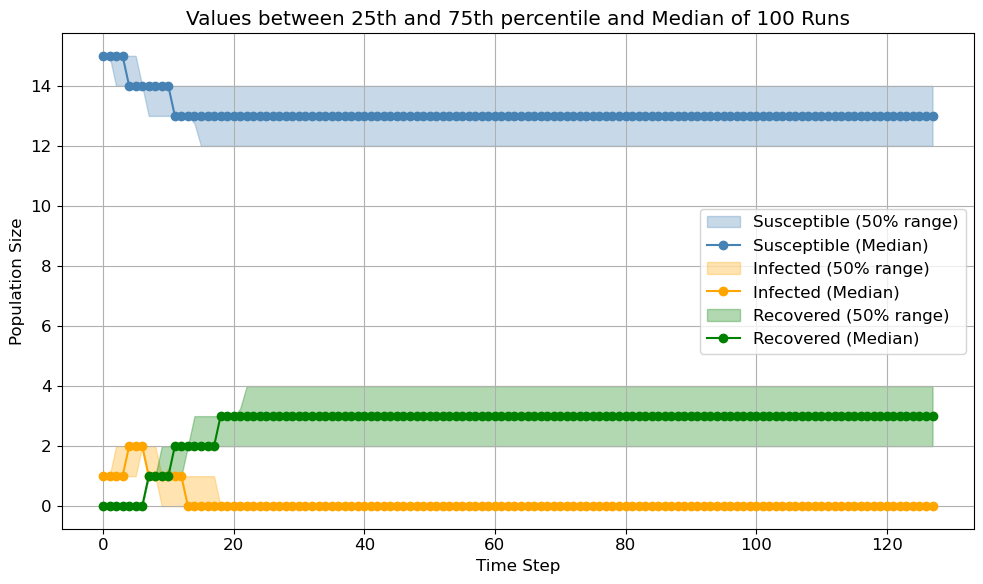
\includegraphics[width=0.3\textwidth]{images/experiments/experiment_016_008_16.png}}
    \hspace*{\fill}
    \subfigure[Population 16, Lifetime 16]{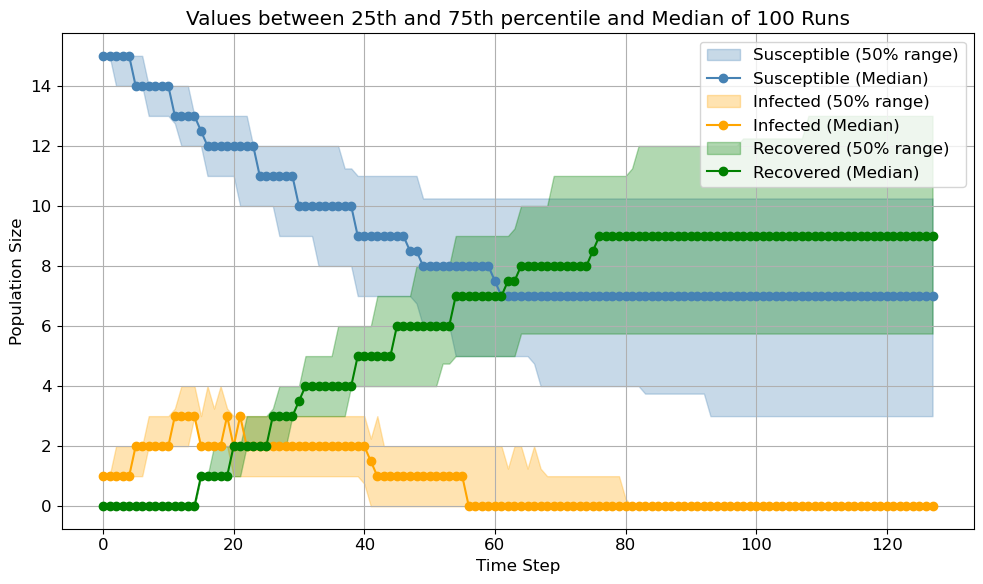
\includegraphics[width=0.3\textwidth]{images/experiments/experiment_016_016_16.png}\label{images/experiments/experiment_016_016_16.png}}
    \hspace*{\fill}
    \subfigure[Population 16, Lifetime 32]{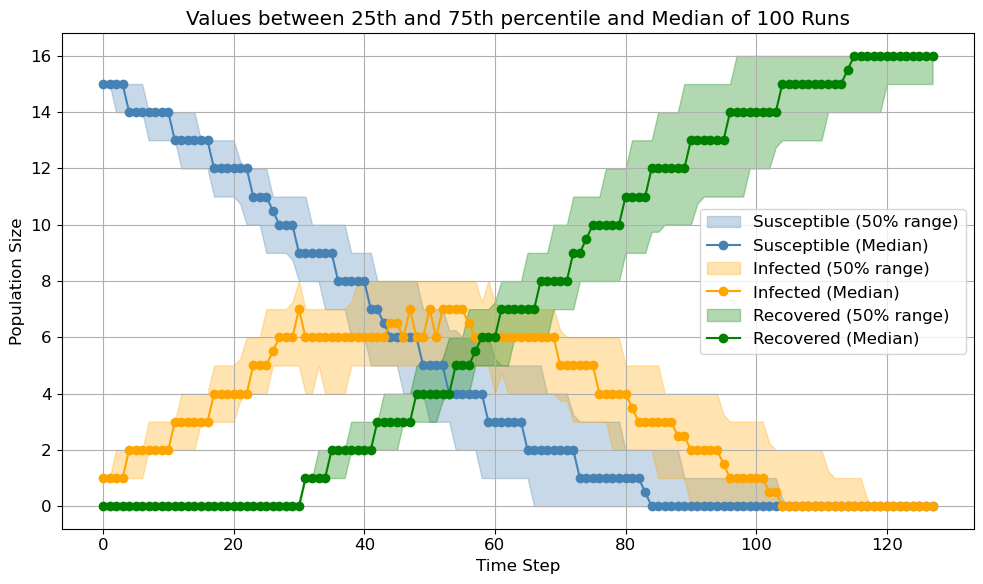
\includegraphics[width=0.3\textwidth]{images/experiments/experiment_016_032_16.png}}

    \subfigure[Population 32, Lifetime 8]{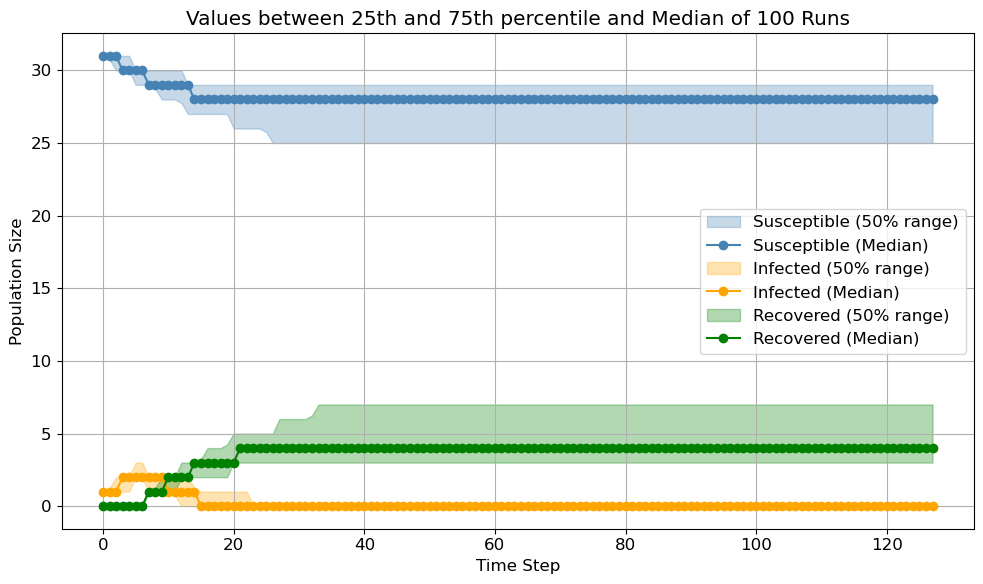
\includegraphics[width=0.3\textwidth]{images/experiments/experiment_032_008_16.png}}
    \hspace*{\fill}
    \subfigure[Population 32, Lifetime 16]{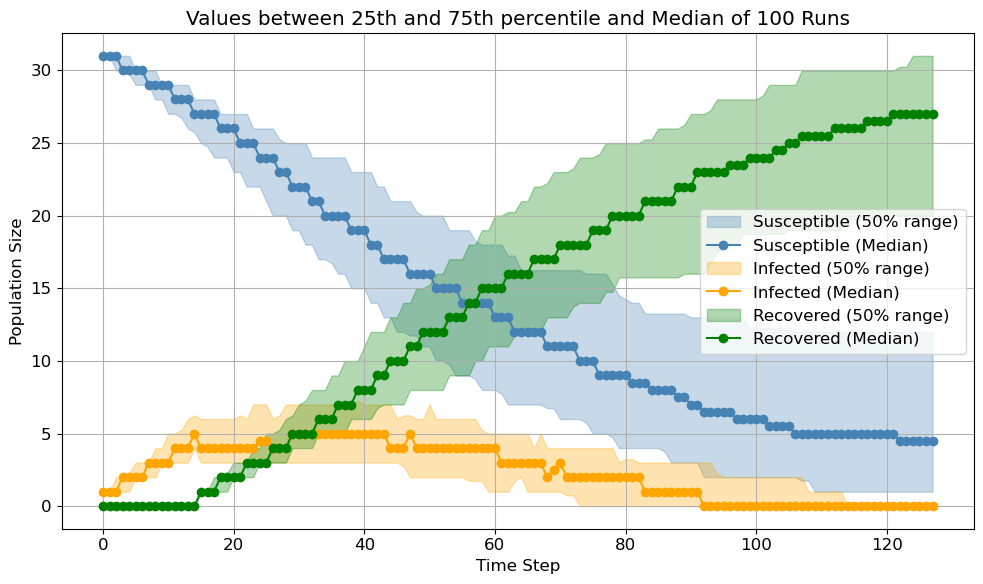
\includegraphics[width=0.3\textwidth]{images/experiments/experiment_032_016_16.png}}
    \hspace*{\fill}
    \subfigure[Population 32, Lifetime 32]{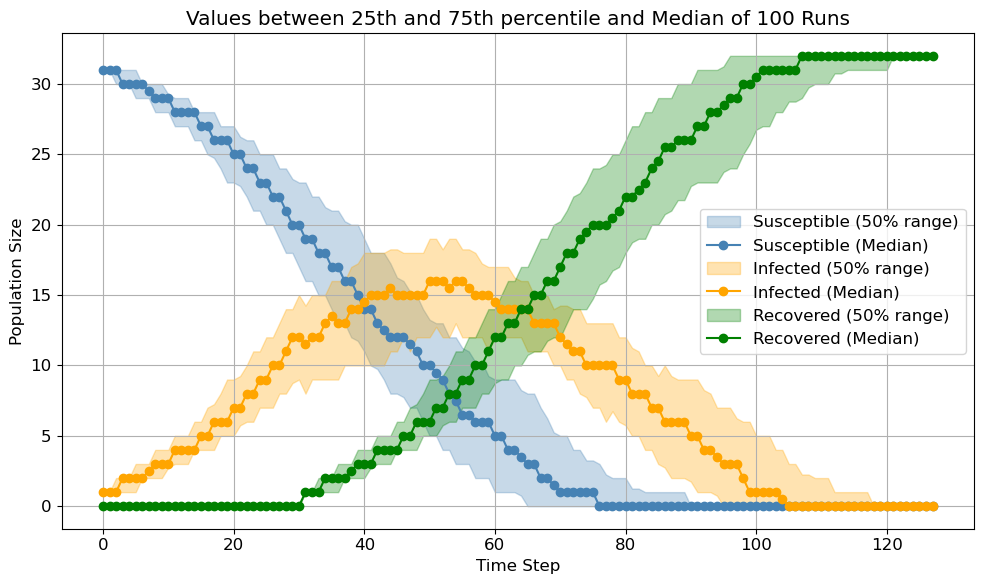
\includegraphics[width=0.3\textwidth]{images/experiments/experiment_032_032_16.png}}

    \subfigure[Population 64, Lifetime 8]{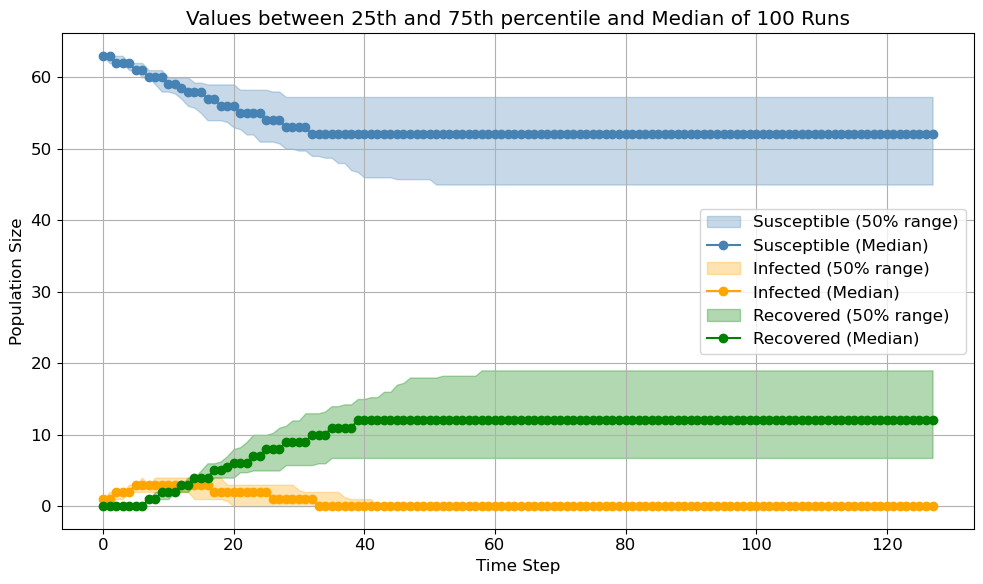
\includegraphics[width=0.3\textwidth]{images/experiments/experiment_064_008_16.png}}
    \hspace*{\fill}
    \subfigure[Population 64, Lifetime 16]{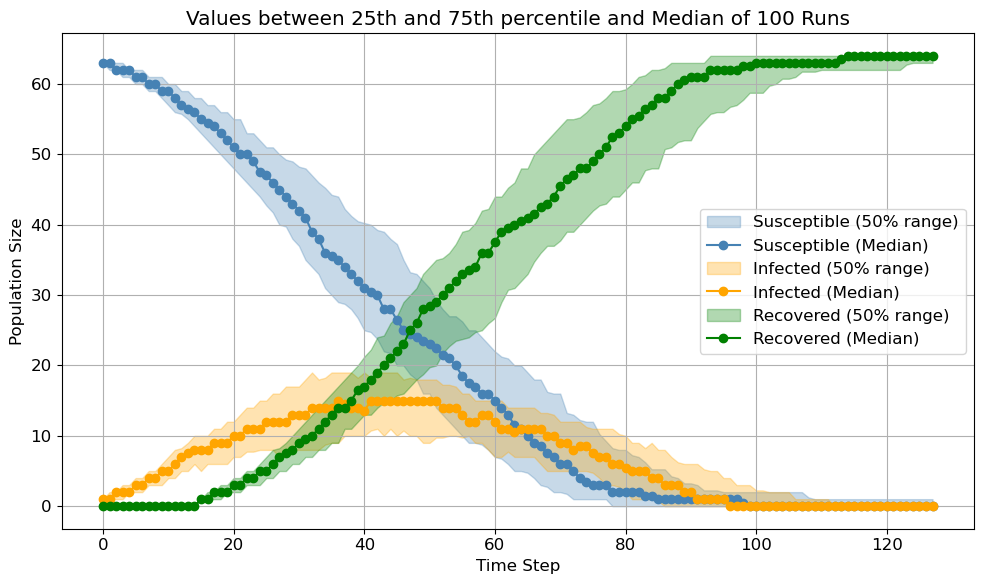
\includegraphics[width=0.3\textwidth]{images/experiments/experiment_064_016_16.png}}
    \hspace*{\fill}
    \subfigure[Population 64, Lifetime 32]{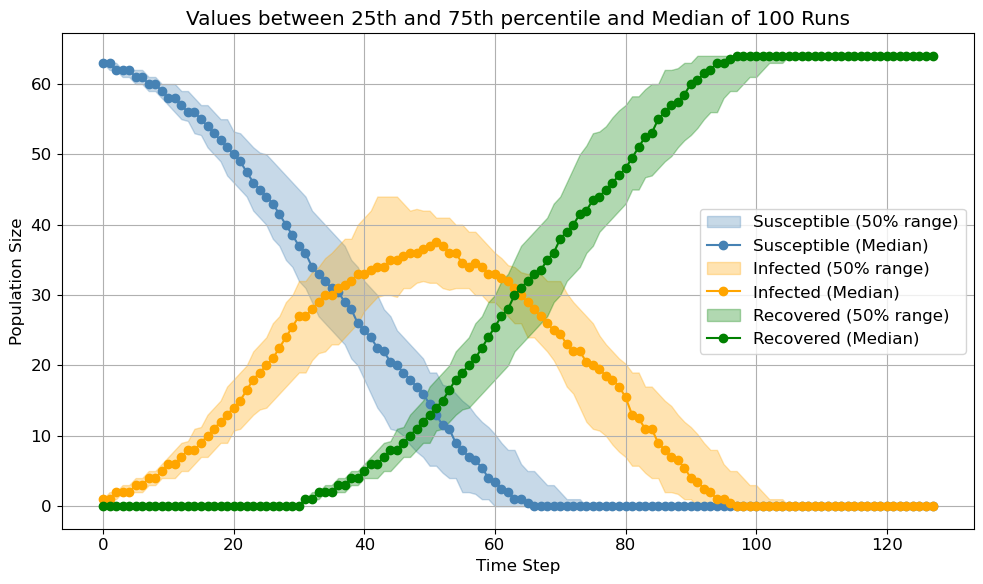
\includegraphics[width=0.3\textwidth]{images/experiments/experiment_064_032_16.png}}

    \subfigure[Population 128, Lifetime 8]{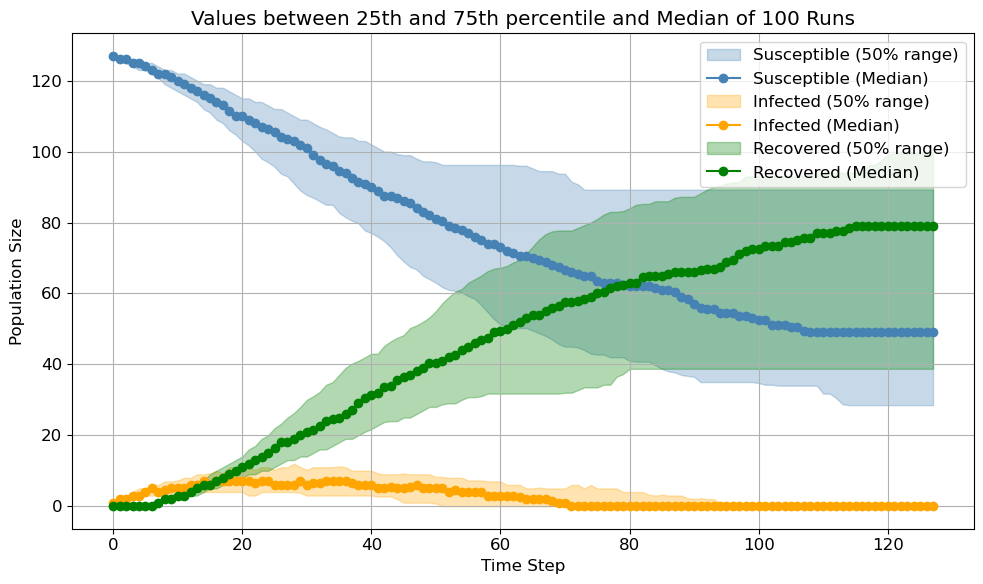
\includegraphics[width=0.3\textwidth]{images/experiments/experiment_128_008_16.png}\label{images/experiments/experiment_128_008_16.png}}
    \hspace*{\fill}
    \subfigure[Population 128, Lifetime 16]{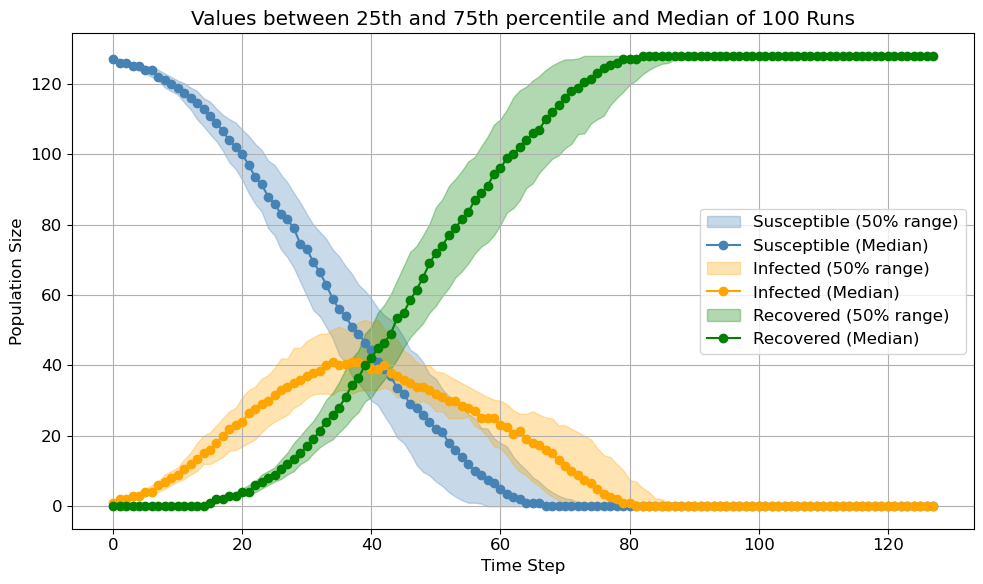
\includegraphics[width=0.3\textwidth]{images/experiments/experiment_128_016_16.png}}
    \hspace*{\fill}
    \subfigure[Population 128, Lifetime 32]{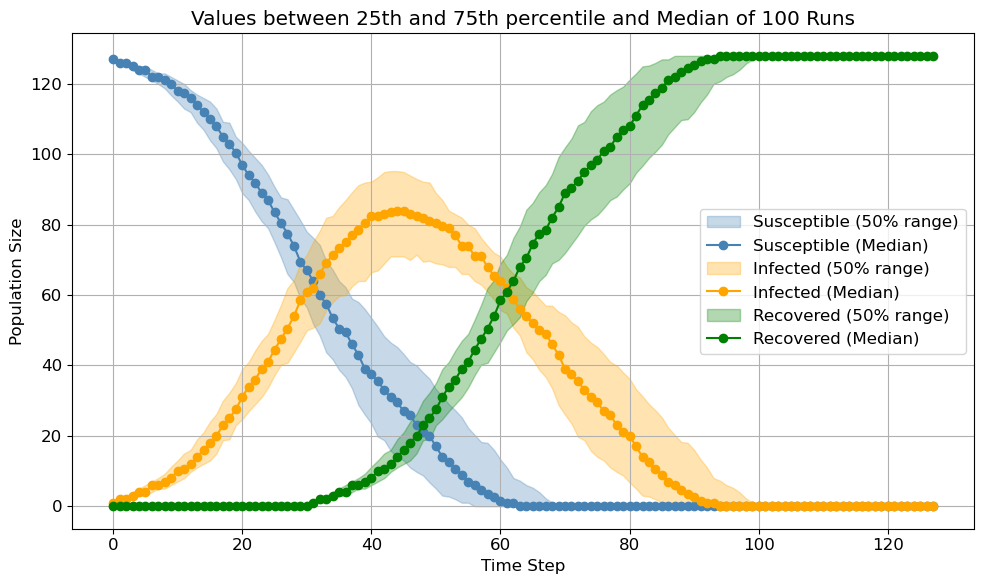
\includegraphics[width=0.3\textwidth]{images/experiments/experiment_128_032_16.png}}

    \caption{Experiment 5 - population density influence on simulation dynamics} \label{fig:experiment5}
\end{figure}

\subsection{Experiment 6 - alternate map topologies}

Simulation of information propagation without taking into account the constraints of the terrain or the shape of the map, is not going to be always representative of real world games and their simulated worlds.
For this reason in this experiment there were created four distinct maps with varying topology and design.
Figures \ref{fig:map1_design}, \ref{fig:map2_design}, \ref{fig:map3_design} and \ref{fig:map4_design} show the different map designs along with their in-simulation graphical representation, showing example distribution of agents on each map.
Map presented on figure \ref{fig:map1_design} represents a complex system of caves with organic wall topology and many narrow corridors.
The second map from figure \ref{fig:map2_design} is a reference map similar to the one used in previous experiments and is simply an empty square of 48 by 48 tiles in size.
Map shown on figure \ref{fig:map3_design} is a connected system of two rooms where the only connection is a narrow corridor that limits the throughput of agents wanting to pass through it to the second half of the map.
Finally, the fourth map visible on figure \ref{fig:map4_design} is a irregular combination of four rooms connected by one central room.
The last map's design was made to determine if irregular but symmetrical design of the map impacts the dynamics of the simulation in a noticable way.

\begin{figure}[H]
    \centering

    \subfigure[design]{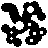
\includegraphics[width=0.48\textwidth]{images/experiments2/map01.png}}
    \hspace*{\fill}
    \subfigure[in-simulation]{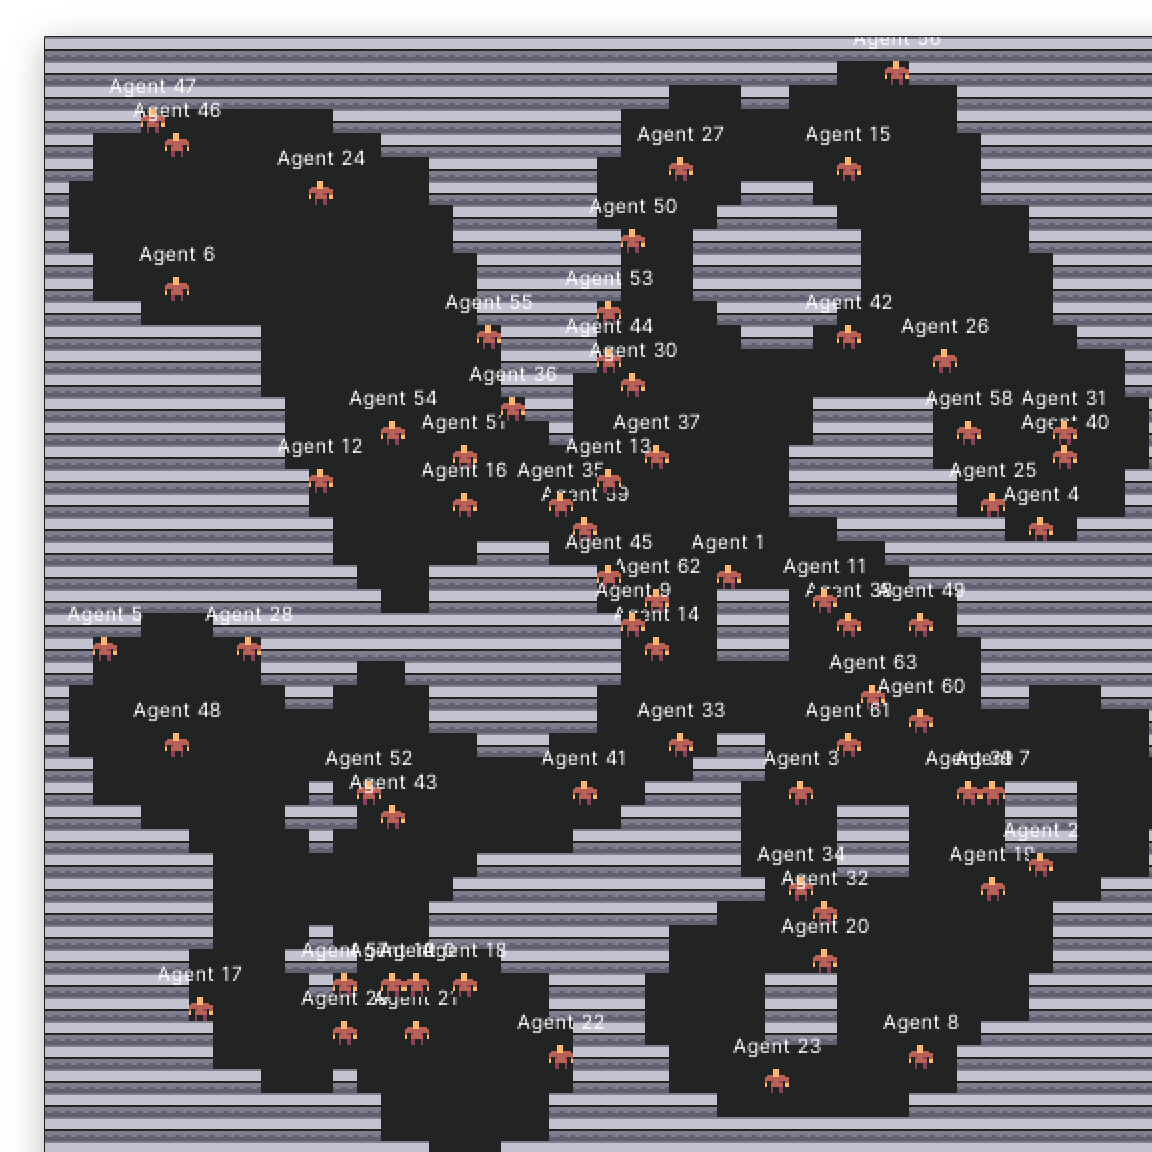
\includegraphics[width=0.48\textwidth]{images/experiments2/sir_map01.png}}

    \caption{Experiment 6 - map 1}\label{fig:map1_design}
\end{figure}

\begin{figure}[H]
    \centering

    \subfigure[design]{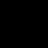
\includegraphics[width=0.48\textwidth]{images/experiments2/map02.png}}
    \hspace*{\fill}
    \subfigure[in-simulation]{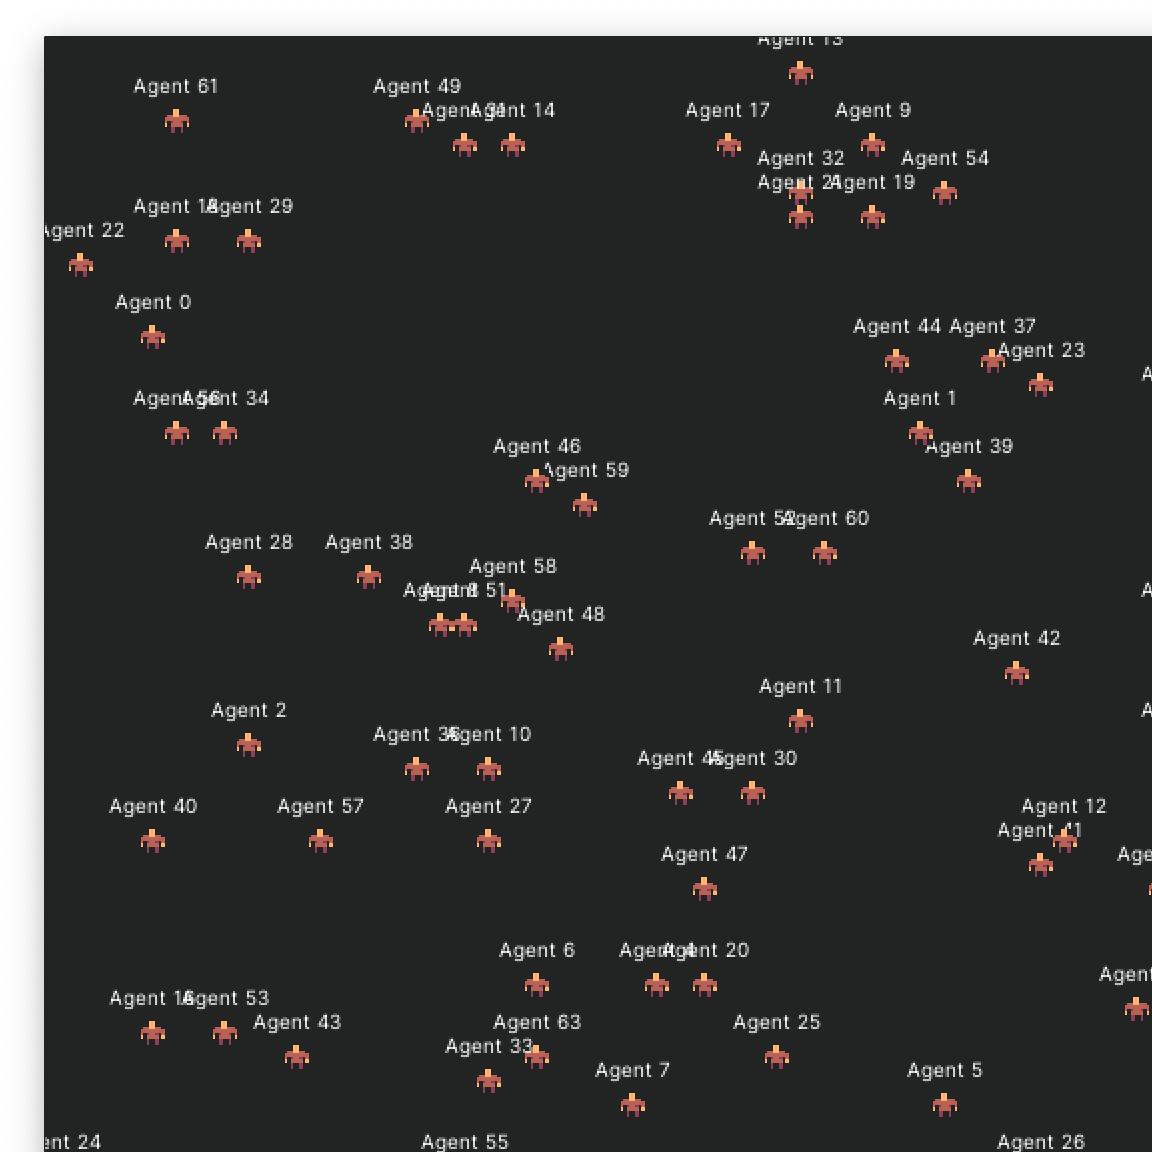
\includegraphics[width=0.48\textwidth]{images/experiments2/sir_map02.png}}

    \caption{Experiment 6 - map 2}\label{fig:map2_design}
\end{figure}

\begin{figure}[H]
    \centering

    \subfigure[design]{
\includegraphics[width=0.48\textwidth]{images/experiments2/map03.png}}
    \hspace*{\fill}
    \subfigure[in-simulation]{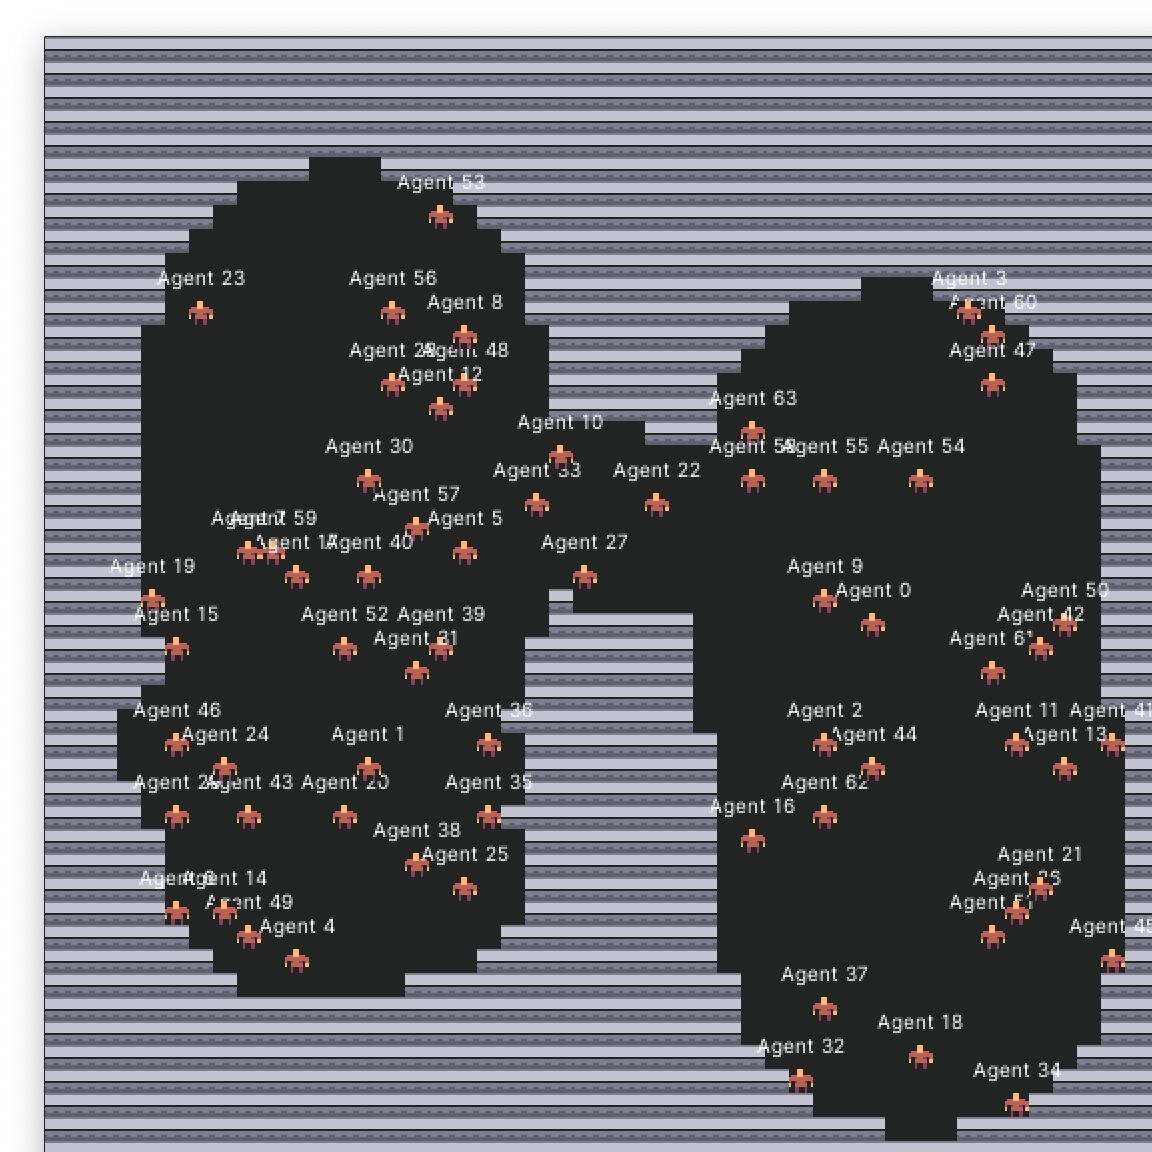
\includegraphics[width=0.48\textwidth]{images/experiments2/sir_map03.png}}

    \caption{Experiment 6 - map 3}\label{fig:map3_design}
\end{figure}

\begin{figure}[H]
    \centering

    \subfigure[design]{
\includegraphics[width=0.48\textwidth]{images/experiments2/map04.png}}
    \hspace*{\fill}
    \subfigure[in-simulation]{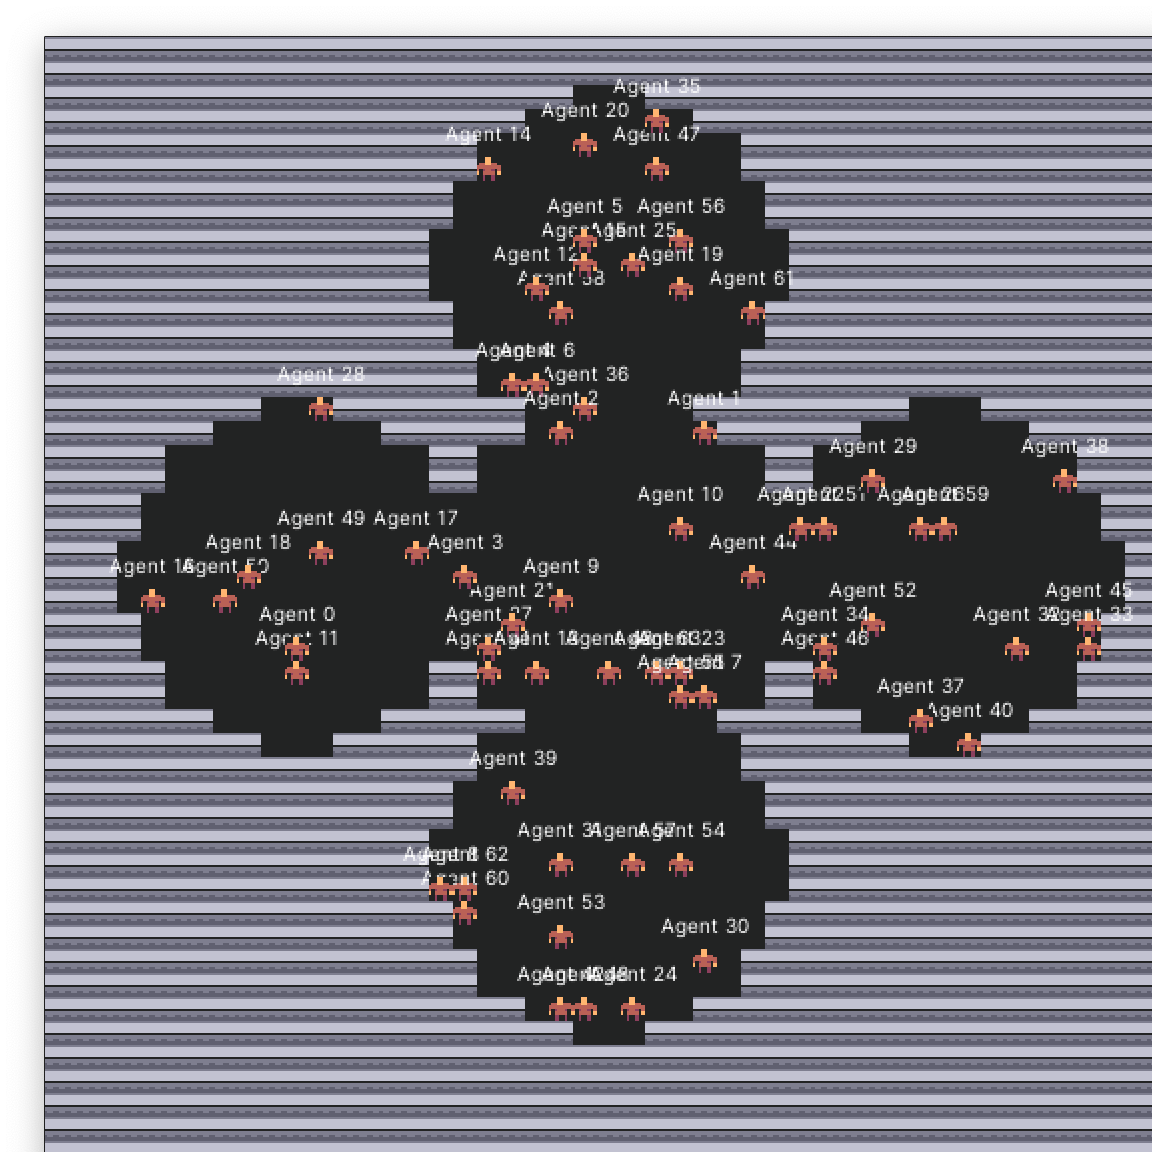
\includegraphics[width=0.48\textwidth]{images/experiments2/sir_map04.png}}

    \caption{Experiment 6 - map 4}\label{fig:map4_design}
\end{figure}

% \begin{figure}[H]
%     \centering

%     \subfigure[Map 1]{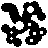
\includegraphics[width=0.3\textwidth]{images/experiments2/map01.png}\label{fig:map1_design}}
%     \hspace*{\fill}
%     \subfigure[Map 1 - in-simulation]{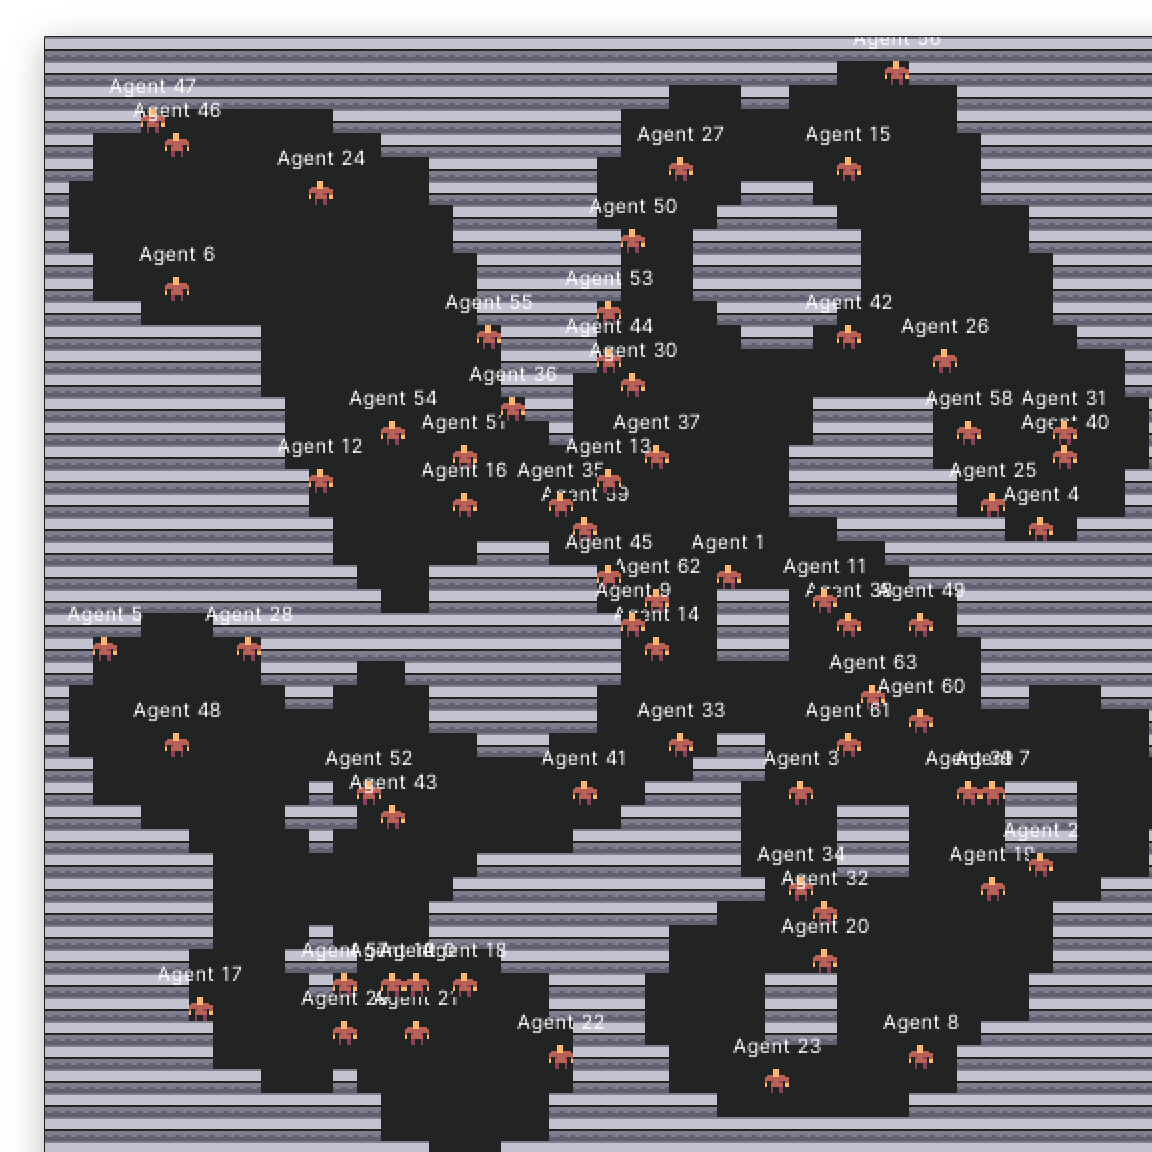
\includegraphics[width=0.3\textwidth]{images/experiments2/sir_map01.png}}

%     \subfigure[Map 2]{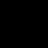
\includegraphics[width=0.3\textwidth]{images/experiments2/map02.png}\label{fig:map2_design}}
%     \hspace*{\fill}
%     \subfigure[Map 2 - in-simulation]{\includegraphics[width=0.3\textwidth]{images/experiments2/sir_map02.png}}

%     \subfigure[Map 3]{\includegraphics[width=0.3\textwidth]{images/experiments2/map03.png}\label{fig:map3_design}}
%     \hspace*{\fill}
%     \subfigure[Map 3 - in-simulation]{\includegraphics[width=0.3\textwidth]{images/experiments2/sir_map03.png}}

%     \subfigure[Map 4]{\includegraphics[width=0.3\textwidth]{images/experiments2/map04.png}\label{fig:map4_design}}
%     \hspace*{\fill}
%     \subfigure[Map 4 - in-simulation]{\includegraphics[width=0.3\textwidth]{images/experiments2/sir_map04.png}}

%     \caption{Experiment 6 - alternate map topologies}\label{fig:maps}
% \end{figure}

The previous experiment proven that the density of population does not impact the dynamics of the simulation in a noticeable way as long as the lifetime of the infected agent is above the threshold necessary for it to travel across to any other agent.
For this reason four simulations of a hundred runs each were selected for comparison on figure \ref{fig:maps_comparison}.
The simulation parameters chosen for this experiment were selected such as to minimize their impact on the dynamics of the simulation in each of the maps.
The lifetime of the infected agents was set to 32 simulation steps and their sight has been set to 16 tiles.
The population in each map is 64 agents, randomly and uniformly distributed across the map inside of the allowed (hollow) spaces.
The rest of the simulation parameters follow the example of previous experiments.

\begin{figure}[H]
    \centering

    \subfigure[Map 1]{\includegraphics[width=0.48\textwidth]{images/experiments2/map01_064_032_16.png}}
    \hspace*{\fill}
    \subfigure[Map 2]{\includegraphics[width=0.48\textwidth]{images/experiments2/map02_064_032_16.png}}

    \subfigure[Map 3]{\includegraphics[width=0.48\textwidth]{images/experiments2/map03_064_032_16.png}}
    \hspace*{\fill}
    \subfigure[Map 4]{\includegraphics[width=0.48\textwidth]{images/experiments2/map04_064_032_16.png}}

    \caption{Experiment 6 - comparison of simulation dynamics between maps}\label{fig:maps_comparison}
\end{figure}

It can be seen that the topology of each map changes slightly the dynamics of the simulation.
It is worth nothing however that while the dynamics differ for each map, the general shape of each series remains comparable.
The major difference is in the width of the shaded area showing the values contained between 25th percentile and 75th percentile.

In order to determine the impact the lifetime parameter, a set of four simulation runs was conducted.
Each map is impacted by the change of simulation parameters in a different way.
Figures \ref{fig:map1_lifetime}, \ref{fig:map2_lifetime}, \ref{fig:map3_lifetime} and \ref{fig:map4_lifetime} show the comparison of four simulations, each with a different value of the lifetime parameter.

\begin{figure}[H]
    \centering

    \subfigure[lifetime 8]{\includegraphics[width=0.48\textwidth]{images/experiments2/map01_064_008_16.png}}
    \hspace*{\fill}
    \subfigure[lifetime 16]{\includegraphics[width=0.48\textwidth]{images/experiments2/map01_064_016_16.png}}

    \subfigure[lifetime 32]{\includegraphics[width=0.48\textwidth]{images/experiments2/map01_064_032_16.png}}
    \hspace*{\fill}
    \subfigure[lifetime 64]{\includegraphics[width=0.48\textwidth]{images/experiments2/map01_064_064_16.png}}

    \caption{Experiment 6 - Map 1 lifetime influence}\label{fig:map1_lifetime}
\end{figure}

The first map shows heavy influence of the lifetime parameter that impacts the dynamics of the simulation.
Because the system of caves is complex and narrow, the agents do not have enough to time to reach other agents and so the propagation stops.

\begin{figure}[H]
    \centering

    \subfigure[lifetime 8]{\includegraphics[width=0.48\textwidth]{images/experiments2/map02_064_008_16.png}}
    \hspace*{\fill}
    \subfigure[lifetime 16]{\includegraphics[width=0.48\textwidth]{images/experiments2/map02_064_016_16.png}}

    \subfigure[lifetime 32]{\includegraphics[width=0.48\textwidth]{images/experiments2/map02_064_032_16.png}}
    \hspace*{\fill}
    \subfigure[lifetime 64]{\includegraphics[width=0.48\textwidth]{images/experiments2/map02_064_064_16.png}}

    \caption{Experiment 6 - Map 2 lifetime influence}\label{fig:map2_lifetime}
\end{figure}

The second map is a reference map that shows results similar to the ones already described in the preceding experiments.
Figure \ref{fig:map2_lifetime} shows much smaller shaded areas when compared to the simulation illustrated on figure \ref{fig:map1_lifetime}.
From this one can see that the complexity of the cave system in comparison with the reference map simulation impacts the repeatability and predictability of each simulation run.

\begin{figure}[H]
    \centering

    \subfigure[lifetime 8]{\includegraphics[width=0.48\textwidth]{images/experiments2/map03_064_008_16.png}}
    \hspace*{\fill}
    \subfigure[lifetime 16]{\includegraphics[width=0.48\textwidth]{images/experiments2/map03_064_016_16.png}}

    \subfigure[lifetime 32]{\includegraphics[width=0.48\textwidth]{images/experiments2/map03_064_032_16.png}}
    \hspace*{\fill}
    \subfigure[lifetime 64]{\includegraphics[width=0.48\textwidth]{images/experiments2/map03_064_064_16.png}}

    \caption{Experiment 6 - Map 3 lifetime influence}\label{fig:map3_lifetime}
\end{figure}

Even though the third map contains a narrow passageway that should impact the simulation's dynamics, the only noticeable difference between the reference simulation from figure \ref{fig:map2_lifetime} is the much less curved shape of the data series from figure \ref{fig:map3_lifetime}.
This could be attributed to the narrow passageway in the middle of the map that impacts the speed of the infection spread in the inflection points.

\begin{figure}[H]
    \centering

    \subfigure[lifetime 8]{\includegraphics[width=0.48\textwidth]{images/experiments2/map04_064_008_16.png}}
    \hspace*{\fill}
    \subfigure[lifetime 16]{\includegraphics[width=0.48\textwidth]{images/experiments2/map04_064_016_16.png}}

    \subfigure[lifetime 32]{\includegraphics[width=0.48\textwidth]{images/experiments2/map04_064_032_16.png}}
    \hspace*{\fill}
    \subfigure[lifetime 64]{\includegraphics[width=0.48\textwidth]{images/experiments2/map04_064_064_16.png}\label{fig:map4_lifetime_d}}

    \caption{Experiment 6 - Map 4 lifetime influence}\label{fig:map4_lifetime}
\end{figure}

The last simulation as shown on figure \ref{fig:map4_lifetime} shows a flat segment of the infected agents on subfigure \ref{fig:map4_lifetime_d}.
This could be attributed to the symmetric but irregular shape of the map.
The same situation does not appear in any of the previous simulations.

In conclusion it can be seen that map topology affects the dynamics of the simulation and is affected by the values of the system's parameters.
The general shape of the resultant simulation dynamics still show similarities to the SIR model which can also be interpreted as the model's applicability in non-homogeneous simulations.

\subsection{Experiment 7 - limited range of movement}

When all agents are constrained to move only within a set distance from their original position the dynamics of information propagation change.
For this experiment the range of the agent's movement is equal to its range of sight.
Figures \ref{fig:map1_range}, \ref{fig:map2_range}, \ref{fig:map3_range} and \ref{fig:map4_range} show the impact on the range limit imposed on each agent on the dynamics of the propagation.

\begin{figure}[H]
    \centering

    \subfigure[range 4]{\includegraphics[width=0.3\textwidth]{images/experiments3/map01_064_032_04.png}}
    \hspace*{\fill}
    \subfigure[range 8]{\includegraphics[width=0.3\textwidth]{images/experiments3/map01_064_032_08.png}}
    \hspace*{\fill}
    \subfigure[range 16]{\includegraphics[width=0.3\textwidth]{images/experiments3/map01_064_032_16.png}}

    \caption{Experiment 6 - Map 1 limited range simulation}\label{fig:map1_range}
\end{figure}

\begin{figure}[H]
    \centering

    \subfigure[range 4]{\includegraphics[width=0.3\textwidth]{images/experiments3/map02_064_032_04.png}}
    \hspace*{\fill}
    \subfigure[range 8]{\includegraphics[width=0.3\textwidth]{images/experiments3/map02_064_032_08.png}}
    \hspace*{\fill}
    \subfigure[range 16]{\includegraphics[width=0.3\textwidth]{images/experiments3/map02_064_032_16.png}}

    \caption{Experiment 6 - Map 2 limited range simulation}\label{fig:map2_range}
\end{figure}

\begin{figure}[H]
    \centering

    \subfigure[range 4]{\includegraphics[width=0.3\textwidth]{images/experiments3/map03_064_032_04.png}}
    \hspace*{\fill}
    \subfigure[range 8]{\includegraphics[width=0.3\textwidth]{images/experiments3/map03_064_032_08.png}}
    \hspace*{\fill}
    \subfigure[range 16]{\includegraphics[width=0.3\textwidth]{images/experiments3/map03_064_032_16.png}}

    \caption{Experiment 6 - Map 3 limited range simulation}\label{fig:map3_range}
\end{figure}

\begin{figure}[H]
    \centering

    \subfigure[range 4]{\includegraphics[width=0.3\textwidth]{images/experiments3/map04_064_032_04.png}}
    \hspace*{\fill}
    \subfigure[range 8]{\includegraphics[width=0.3\textwidth]{images/experiments3/map04_064_032_08.png}}
    \hspace*{\fill}
    \subfigure[range 16]{\includegraphics[width=0.3\textwidth]{images/experiments3/map04_064_032_16.png}}

    \caption{Experiment 6 - Map 4 limited range simulation}\label{fig:map4_range}
\end{figure}

The reference map from figure \ref{fig:map2_range} shows that the moment when first recovery of an agent starts, the infection rate starts rapidly falling down.
This behavior can be likewise noticed on all of the simulations in this experiment.
The range constraint heavily impacts the dynamics of the simulation by greatly reducing the efficiency of propagation.

\begin{figure}[H]
    \centering

    \subfigure[lifetime 8]{\includegraphics[width=0.48\textwidth]{images/experiments3/map01_064_008_08.png}}
    \hspace*{\fill}
    \subfigure[lifetime 16]{\includegraphics[width=0.48\textwidth]{images/experiments3/map01_064_016_08.png}}

    \subfigure[lifetime 32]{\includegraphics[width=0.48\textwidth]{images/experiments3/map01_064_032_08.png}}
    \hspace*{\fill}
    \subfigure[lifetime 64]{\includegraphics[width=0.48\textwidth]{images/experiments3/map01_064_064_08.png}}

    \caption{Experiment 6 - Map 1 limited lifetime influence on limited range simulation (range 8)}\label{fig:map1_lifetime_range}
\end{figure}

\begin{figure}[H]
    \centering

    \subfigure[lifetime 8]{\includegraphics[width=0.48\textwidth]{images/experiments3/map02_064_008_08.png}}
    \hspace*{\fill}
    \subfigure[lifetime 16]{\includegraphics[width=0.48\textwidth]{images/experiments3/map02_064_016_08.png}}

    \subfigure[lifetime 32]{\includegraphics[width=0.48\textwidth]{images/experiments3/map02_064_032_08.png}}
    \hspace*{\fill}
    \subfigure[lifetime 64]{\includegraphics[width=0.48\textwidth]{images/experiments3/map02_064_064_08.png}}

    \caption{Experiment 6 - Map 2 limited lifetime influence on limited range simulation (range 8)}\label{fig:map2_lifetime_range}
\end{figure}

\begin{figure}[H]
    \centering

    \subfigure[lifetime 8]{\includegraphics[width=0.48\textwidth]{images/experiments3/map03_064_008_08.png}}
    \hspace*{\fill}
    \subfigure[lifetime 16]{\includegraphics[width=0.48\textwidth]{images/experiments3/map03_064_016_08.png}}

    \subfigure[lifetime 32]{\includegraphics[width=0.48\textwidth]{images/experiments3/map03_064_032_08.png}}
    \hspace*{\fill}
    \subfigure[lifetime 64]{\includegraphics[width=0.48\textwidth]{images/experiments3/map03_064_064_08.png}}

    \caption{Experiment 6 - Map 3 limited lifetime influence on limited range simulation (range 8)}\label{fig:map3_lifetime_range}
\end{figure}

\begin{figure}[H]
    \centering

    \subfigure[lifetime 8]{\includegraphics[width=0.48\textwidth]{images/experiments3/map04_064_008_08.png}}
    \hspace*{\fill}
    \subfigure[lifetime 16]{\includegraphics[width=0.48\textwidth]{images/experiments3/map04_064_016_08.png}}

    \subfigure[lifetime 32]{\includegraphics[width=0.48\textwidth]{images/experiments3/map04_064_032_08.png}}
    \hspace*{\fill}
    \subfigure[lifetime 64]{\includegraphics[width=0.48\textwidth]{images/experiments3/map04_064_064_08.png}}

    \caption{Experiment 6 - Map 4 limited lifetime influence on limited range simulation (range 8)}\label{fig:map4_lifetime_range}
\end{figure}

In order to determine the impact of lifetime parameter, four additional experimentations were conducted on each map.
The results are visible on figures \ref{fig:map1_lifetime_range}, \ref{fig:map2_lifetime_range}, \ref{fig:map3_lifetime_range} and \ref{fig:map4_lifetime_range}.

It can be seen that in nearly all maps the lifetime parameter does not really impact the simulation outcome.
The most heavily impacted map are the third and the fourth one, the results from which are on figures \ref{fig:map3_lifetime_range} and \ref{fig:map4_lifetime_range}.
This could be attributed to the higher population density on these maps as the same population size is distributed on a smaller area.
The conditions of this experiment are heavily impacted by population density as opposed to the previous experiments that relied mostly on the combination of agent's sight (but only up to a certain threshold) and lifetime of infected individuals.

\begin{figure}[H]
    \centering

    \subfigure[map 1]{\includegraphics[width=0.48\textwidth]{images/experiments3/map01_064_032_08.png}}
    \hspace*{\fill}
    \subfigure[map 2]{\includegraphics[width=0.48\textwidth]{images/experiments3/map02_064_032_08.png}}

    \subfigure[map 3]{\includegraphics[width=0.48\textwidth]{images/experiments3/map03_064_032_08.png}\label{fig:maps_limited_range_3}}
    \hspace*{\fill}
    \subfigure[map 4]{\includegraphics[width=0.48\textwidth]{images/experiments3/map04_064_032_08.png}\label{fig:maps_limited_range_4}}

    \caption{Experiment 6 - comparison of maps' dynamics at lifetime 32 and range 8}\label{fig:maps_limited_range}
\end{figure}

Lastly, the figure \ref{fig:maps_limited_range} shows comparison of all four maps experiments run under the parameters of lifetime equal to 32 and range limited to 8 tiles.
The results confirm the theory that this experiment is mostly influenced by population density as the only two maps with most defined propagation dynamics are those represented by figures \ref{fig:maps_limited_range_3} and \ref{fig:maps_limited_range_4}.
One noteworthy aspect of the fourth map's result is the large shaded area on the graph that shows the high spread of values, even between 25th and 75th percentile.
This can be attributed to random distribution producing unpredictable results that are amplified under the conditions of this experiment.
% Additionally, a peculiar behavior could be noticed where a combination of limited lifetime and range caused propagation in swirling motion.

\section{Conclusions}

The experiments show that the implemented multi-agent system is capable of producing simulation dynamics that correlate with those of the chosen epidemiological model.
The system's parameter representing the lifetime of the infected individual (or in terms of information propagation the time when the individual is still interested in the information that it knows) is directly correlated with the recovery rate in the SIR model.
While the individual rules act only on the agent itself, the whole system exhibits emergent behavior of a real population that can be described using a real compartmental epidemiological model.
This answers the second research question regarding the ability of the system to exhibit similar dynamics to that of the comparable mathematical model.
Results clearly show that multi-agent systems can be used to simulate populations in which the information (and infection) propagation dynamics follow dynamics of epidemiological models used in modeling of real populations.